\documentclass[a4paper,onecolumn,oneside,12pt,extrafontsizes]{memoir}
%  W celu przygotowania wydruku do archiwum można:
%  a) przygotować pdf, w którym dwie strony zostaną wstawione na jedną fizyczną stronę i taki dokument wydrukować dwustronnie (podejście zalecane)
%
%   Taki dokument można przygotować poprzez
%   - wydruk z Adobe Acrobat Reader z opcją "Wiele" - sekcja "Rozmiar i obsługa stron"
%   - wykorzystanie narzędzi psutils
%
%      Windows (zakładając, że w dystrybucji MiKTeX jest pakiet miktex-psutils-bin-x64-2.9):
%        "c:\Program Files\MiKTeX 2.9\miktex\bin\x64\pdf2ps.exe" Dyplom.pdf Dyplom.ps
%        "c:\Program Files\MiKTeX 2.9\miktex\bin\x64\psnup.exe" -2 Dyplom.ps Dyplom2.ps
%        "c:\Program Files\MiKTeX 2.9\miktex\bin\x64\ps2pdf.exe" Dyplom2.ps Dyplom2.pdf
%        Del Dyplom2.ps Dyplom.ps
%
%     Linux:
%        pdf2ps Dyplom.pdf - | psnup -2 | ps2pdf - Dyplom2.pdf
%
%  b) przekomplilować dokument zmniejszając czcionkę (podejście niezalecane, bo zmienia formatowanie dokumentu)
%
%    Do tego wystarczy posłużyć się poniższymi komendami (zamiast documentclass z pierwszej linijki):
%   \documentclass[a4paper,onecolumn,twoside,10pt]{memoir} 
%   \renewcommand{\normalsize}{\fontsize{8pt}{10pt}\selectfont}

%\usepackage[cp1250]{inputenc} % Proszę zostawić, jeśli kodowanie edytowanych plików to cp1250 
\usepackage[utf8]{inputenc} % Proszę użyć zamiast powyższego, jeśli kodowanie edytowanych plików to UTF8
\usepackage[T1]{fontenc}
\usepackage[english,polish]{babel} % Tutaj ważna jest kolejność atrybutów (dla pracy po polsku polish powinno być na końcu)
%\DisemulatePackage{setspace}
\usepackage{setspace}
\usepackage{color,calc}
%\usepackage{soul} % pakiet z komendami do podkreślania, przekreślania, podświetlania tekstu (raczej niepotrzebny)
\usepackage{ebgaramond} % pakiet z czcionkami garamond, potrzebny tylko do strony tytułowej, musi wystąpić przed pakietem tgtermes

%% Aby uzyskać polskie literki w pdfie (a nie zlepki) korzystamy z pakietu czcionek tgterms. 
%% W pakiecie tym są zdefiniowane klony czcionek Times o kształtach: normalny, pogrubiony, italic, italic pogrubiony.
%% W pakiecie tym brakuje czcionki o kształcie: slanted (podobny do italic). 
%% Jeśli w dokumencie gdzieś zostanie zastosowana czcionka slanted (np. po użyciu komendy \textsl{}), to
%% latex dokona podstawienia na czcionkę standardową i zgłosi to w ostrzeżeniu (warningu).
%% Ponadto tgtermes to czcionka do tekstu. Wszelkie matematyczne wzory będą sformatowane domyślną czcionką do wzorów.
%% Jeśli wzory mają być sformatowane z wykorzystaniem innych czcionek, trzeba to jawnie zadeklarować.

%% Po zainstalowaniu pakietu tgtermes może będzie trzeba zauktualizować informacje 
%% o dostępnych fontach oraz mapy. Można to zrobić z konsoli (jako administrator)
%% initexmf --admin --update-fndb
%% initexmf --admin --mkmaps

\usepackage{tgtermes}   
\renewcommand*\ttdefault{txtt}


%%%%%%%%%%%%%%%%%%%%%%%%%%%%%%%%%%%%%%%%%%%%%%%%%%%%%%%%%%%%%%%%%%%%%%%%%%%%%%%%
%% Ustawienia odpowiedzialne za sposób łamania dokumentu
%% i ułożenie elementów pływających
%%%%%%%%%%%%%%%%%%%%%%%%%%%%%%%%%%%%%%%%%%%%%%%%%%%%%%%%%%%%%%%%%%%%%%%%%%%%%%%%
%\hyphenpenalty=10000		% nie dziel wyrazów zbyt często
\clubpenalty=10000      % kara za sierotki
\widowpenalty=10000     % nie pozostawiaj wdów
%\brokenpenalty=10000		% nie dziel wyrazów między stronami - trzeba było wyłączyć, bo nie łamały się linie w lstlisting
%\exhyphenpenalty=999999		% nie dziel słów z myślnikiem - trzeba było wyłączyć, bo nie łamały się linie w lstlisting
\righthyphenmin=3			  % dziel minimum 3 litery

%\tolerance=4500
%\pretolerance=250
%\hfuzz=1.5pt
%\hbadness=1450

\renewcommand{\topfraction}{0.95}
\renewcommand{\bottomfraction}{0.95}
\renewcommand{\textfraction}{0.05}
\renewcommand{\floatpagefraction}{0.35}

%%%%%%%%%%%%%%%%%%%%%%%%%%%%%%%%%%%%%%%%%%%%%%%%%%%%%%%%%%%%%%%%%%%%%%%%%%%%%%%%
%%  Ustawienia rozmiarów: tekstu, nagłówka i stopki, marginesów
%%  dla dokumentów klasy memoir 
%%%%%%%%%%%%%%%%%%%%%%%%%%%%%%%%%%%%%%%%%%%%%%%%%%%%%%%%%%%%%%%%%%%%%%%%%%%%%%%%
\setlength{\headsep}{10pt} 
\setlength{\headheight}{13.6pt} % wartość baselineskip dla czcionki 11pt tj. \small wynosi 13.6pt
\setlength{\footskip}{\headsep+\headheight}
\setlength{\uppermargin}{\headheight+\headsep+1cm}
\setlength{\textheight}{\paperheight-\uppermargin-\footskip-1.5cm}
\setlength{\textwidth}{\paperwidth-5cm}
\setlength{\spinemargin}{2.5cm}
\setlength{\foremargin}{2.5cm}
\setlength{\marginparsep}{2mm}
\setlength{\marginparwidth}{2.3mm}
%\settrimmedsize{297mm}{210mm}{*}
%\settrims{0mm}{0mm}	
\checkandfixthelayout[fixed] % konieczne, aby się dobrze wszystko poustawiało
%%%%%%%%%%%%%%%%%%%%%%%%%%%%%%%%%%%%%%%%%%%%%%%%%%%%%%%%%%%%%%%%%%%%%%%%%%%%%%%%
%%  Ustawienia odległości linii, wcięć, odstępów
%%%%%%%%%%%%%%%%%%%%%%%%%%%%%%%%%%%%%%%%%%%%%%%%%%%%%%%%%%%%%%%%%%%%%%%%%%%%%%%%
\linespread{1}
%\linespread{1.241}
\setlength{\parindent}{14.5pt}


\usepackage{multicol} % pakiet umożliwiający stworzenie wielokolumnowego tekstu
%%%%%%%%%%%%%%%%%%%%%%%%%%%%%%%%%%%%%%%%%%%%%%%%%%%%%%%%%%%%%%%%%%%%%%%%%%%%%%%%
%% Pakiety do formatowania tabel
%%%%%%%%%%%%%%%%%%%%%%%%%%%%%%%%%%%%%%%%%%%%%%%%%%%%%%%%%%%%%%%%%%%%%%%%%%%%%%%%
\usepackage{tabularx}
% Proszę używać tylko tabularx. Innych pakietów proszę nie stosować !!!
% Dokument na pewno da się zredagować bez ich użycia.
%\usepackage{longtable}
%\usepackage{ltxtable}
%\usepackage{tabulary}

%%%%%%%%%%%%%%%%%%%%%%%%%%%%%%%%%%%%%%%%%%%%%%%%%%%%%%%%%%%%%%%%%%%%%%%%%%%%%%%%
%% Pakiet do wstawiania fragmentów kodu
%%%%%%%%%%%%%%%%%%%%%%%%%%%%%%%%%%%%%%%%%%%%%%%%%%%%%%%%%%%%%%%%%%%%%%%%%%%%%%%%
\usepackage{listings} 
\usepackage{xpatch}
\makeatletter
\xpatchcmd\l@lstlisting{1.5em}{0em}{}{}
\makeatother
% Pakiet dostarcza otoczenia lstlisting. Jest ono wysoce konfigurowalne. 
% Konfigurować można indywidualnie każdy z listingów lub globalnie, w poleceniu \lstset{}.

% Zalecane jest, by kod źródłowy był wyprowadzany z użyciem czcionki maszynowej \ttfamily
% Ponieważ kod źródłowy, nawet po obcięciu do interesujących fragmentów, bywa obszerny, należy zmniejszyć czcionkę.
% Zalecane jest \small (dla krótkich fragmentów) oraz \footnotesize (dla dłuższych fragmentów).

% Ponadto podczas konfiguracji można zadeklarować sposób numerowania linii. Numerowanie linii zalecane jest jednak 
% tylko w przypadkach, gdy w redagowanym tekście znajdują się jakieś odwołania do konkretnych linii.
% Jeśli takich odwołań nie ma, numerowanie linii jest zbędne. Proszę wtedy go nie stosować.
% Przy włączaniu numerowania linii należy zwrócić uwagę na to, gdzie pojawią się te numery.
% Bez zmiany dodatkowych parametrów pojawiają się one na marginesie strony (co jest niepożądane).

\lstset{
  basicstyle=\small\ttfamily, % lub basicstyle=\footnotesize\ttfamily
  columns=fullflexible,
	%%showstringspaces=false,
	%%showspaces=false,
  breaklines=true,
  postbreak=\mbox{\textcolor{red}{$\hookrightarrow$}\space}, 
  numbers=left,  % ta i poniższe linie dotyczą ustawienia numerowania i sposobu jego wyprowadzania
  firstnumber=1, 
  numberfirstline=true, 
	xleftmargin=17pt,
  framexleftmargin=17pt,
  framexrightmargin=5pt,
  framexbottommargin=4pt,
	belowskip=.5\baselineskip,
	literate={\_}{{\_\allowbreak}}1 % ta deklaracja przydaje się, jeśli na listingu mają być łamane nazwy zawierające podkreślniki
}

% Jeśli edytowany plik nie jest w kodowaniu cp1250, to jest problem z polskimi znakami występującymi we wstawianym kodzie.
% Dlatego podczas pracy na plikach w kodowaniu UTF8 trzeba zadeklarować mapowanie jak niżej (wystarczy odmarkować).
% Niestety, jak się zastosuje to mapowanie mogą pojawić się problemy z podświetlaniem składni (patrz dalej).
\lstset{literate=%-
{ą}{{\k{a}}}1 {ć}{{\'c}}1 {ę}{{\k{e}}}1 {ł}{{\l{}}}1 {ń}{{\'n}}1 {ó}{{\'o}}1 {ś}{{\'s}}1 {ż}{{\.z}}1 {ź}{{\'z}}1 {Ą}{{\k{A}}}1 {Ć}{{\'C}}1 {Ę}{{\k{E}}}1 {Ł}{{\L{}}}1 {Ń}{{\'N}}1 {Ó}{{\'O}}1 {Ś}{{\'S}}1 {Ż}{{\.Z}}1 {Ź}{{\'Z}}1 
    {Ö}{{\"O}}1
    {Ä}{{\"A}}1
    {Ü}{{\"U}}1
    {ß}{{\ss}}1
    {ü}{{\"u}}1
    {ä}{{\"a}}1
    {ö}{{\"o}}1
    {~}{{\textasciitilde}}1
		{—}{{{\textemdash} }}1
}%{\ \ }{{\ }}1}


%% lstlisting pozwala na ostylowania podświetlania składni wybranych języków.
%% Działa to na zasadzie zdefiniowania słów kluczowych oraz sposobu ich wyświetlania.
%% Ponieważ jest to prosty mechanizm, czasem trudno osiągnąć takie efekty, jakie dają narzędzia IDE. 
%% Jednak w większości przypadku osiągane rezutlaty są zadowalające.


%% lstlisting obsługuje domyślnie kilka najpopularniejszych języków.
%%\lstloadlanguages{% Check Dokumentation for further languages ...
%%C,
%%C++,
%%csh,
%%Java
%%}
%% Inne języki muszą być dodefiniowane. Poniżej podano przykłady definicji języków i styli.

\definecolor{lightgray}{rgb}{.9,.9,.9}
\definecolor{darkgray}{rgb}{.4,.4,.4}
\definecolor{purple}{rgb}{0.65, 0.12, 0.82}
\definecolor{javared}{rgb}{0.6,0,0} % for strings
\definecolor{javagreen}{rgb}{0.25,0.5,0.35} % comments
\definecolor{javapurple}{rgb}{0.5,0,0.35} % keywords
\definecolor{javadocblue}{rgb}{0.25,0.35,0.75} % javadoc
 
\lstdefinelanguage{JavaScript}{ 
	keywords={typeof, new, true, false, catch, function, return, null, catch, switch, var, if, in, while, do, else, case, break},
	keywordstyle=\color{blue}\bfseries,
	ndkeywords={class, export, boolean, throw, implements, import, this},
	ndkeywordstyle=\color{darkgray}\bfseries,
	identifierstyle=\color{black},
	sensitive=false,
	comment=[l]{//},
	morecomment=[s]{/*}{*/},
	commentstyle=\color{purple}\ttfamily,
	stringstyle=\color{red}\ttfamily,
	morestring=[b]',
	morestring=[b]"
}
\lstdefinestyle{JavaScriptStyle}{
	language=JavaScript,
	commentstyle=\color{javagreen}, % niestety, jeśli w linii komentarza pojawią się słowa kluczowe, to zostaną pokolorowane
	backgroundcolor=,%\color{lightgray}, % można ustwić kolor tła, ale jest to niezalecane
	extendedchars=true,
	basicstyle=\footnotesize\ttfamily,
	showstringspaces=false,
	showspaces=false,
	numbers=none,%left,
	numberstyle=\footnotesize,
	numbersep=9pt,
	tabsize=2,
	breaklines=true,
	showtabs=false,
	captionpos=t
}
\lstdefinestyle{JavaStyle}{
basicstyle=\footnotesize\ttfamily,
keywordstyle=\color{javapurple}\bfseries,
stringstyle=\color{javared},
commentstyle=\color{javagreen},
morecomment=[s][\color{javadocblue}]{/**}{*/},
numbers=none,%left,
numberstyle=\tiny\color{black},
stepnumber=1,
numbersep=10pt,
tabsize=4,
showspaces=false,
showstringspaces=false,
captionpos=t
columns=fullflexible,
	%%showstringspaces=false,
	%%showspaces=false,
  breaklines=true,
  postbreak=\mbox{\textcolor{red}{$\hookrightarrow$}\space}, 
  numbers=left,  % ta i poniższe linie dotyczą ustawienia numerowania i sposobu jego wyprowadzania
  firstnumber=1, 
  numberfirstline=true, 
	xleftmargin=17pt,
  framexleftmargin=17pt,
  framexrightmargin=5pt,
  framexbottommargin=4pt,
	belowskip=.5\baselineskip
}

\definecolor{pblue}{rgb}{0.13,0.13,1}
\definecolor{pgreen}{rgb}{0,0.5,0}
\definecolor{pred}{rgb}{0.9,0,0}
\definecolor{pgrey}{rgb}{0.46,0.45,0.48}
\definecolor{dark-grey}{rgb}{0.4,0.4,0.4}
% styl json
\newcommand\JSONnumbervaluestyle{\color{blue}}
\newcommand\JSONstringvaluestyle{\color{red}}

\newif\ifcolonfoundonthisline

\makeatletter

\lstdefinestyle{json-style}  
{
	showstringspaces    = false,
	keywords            = {false,true},
	alsoletter          = 0123456789.,
	morestring          = [s]{"}{"},
	stringstyle         = \ifcolonfoundonthisline\JSONstringvaluestyle\fi,
	MoreSelectCharTable =%
	\lst@DefSaveDef{`:}\colon@json{\processColon@json},
	basicstyle          = \footnotesize\ttfamily,
	keywordstyle        = \ttfamily\bfseries,
	numbers				= left, % zakomentować, jeśli numeracja linii jest niepotrzebna
	numberstyle={\footnotesize\ttfamily\color{dark-grey}},
	xleftmargin			= 2em % zakomentować, jeśli numeracja linii jest niepotrzebna
}

\newcommand\processColon@json{%
	\colon@json%
	\ifnum\lst@mode=\lst@Pmode%
	\global\colonfoundonthislinetrue%
	\fi
}

\lst@AddToHook{Output}{%
	\ifcolonfoundonthisline%
	\ifnum\lst@mode=\lst@Pmode%
	\def\lst@thestyle{\JSONnumbervaluestyle}%
	\fi
	\fi
	\lsthk@DetectKeywords% 
}

\lst@AddToHook{EOL}%
{\global\colonfoundonthislinefalse}

\makeatother

%%\definecolor{red}{rgb}{0.6,0,0} % for strings
%%\definecolor{blue}{rgb}{0,0,0.6}
%%\definecolor{green}{rgb}{0,0.8,0}
%%\definecolor{cyan}{rgb}{0.0,0.6,0.6}
%%
%%\lstdefinestyle{sqlstyle}{
%%language=SQL,
%%basicstyle=\footnotesize\ttfamily, 
%%numbers=left, 
%%numberstyle=\tiny, 
%%numbersep=5pt, 
%%tabsize=2, 
%%extendedchars=true, 
%%breaklines=true, 
%%showspaces=false, 
%%showtabs=true, 
%%xleftmargin=17pt,
%%framexleftmargin=17pt,
%%framexrightmargin=5pt,
%%framexbottommargin=4pt,
%%keywordstyle=\color{blue}, 
%%commentstyle=\color{green}, 
%%stringstyle=\color{red}, 
%%}
%%
%%\lstdefinestyle{sharpcstyle}{
%%language=[Sharp]C,
%%basicstyle=\footnotesize\ttfamily, 
%%numbers=left, 
%%numberstyle=\tiny, 
%%numbersep=5pt, 
%%tabsize=2, 
%%extendedchars=true, 
%%breaklines=true, 
%%showspaces=false, 
%%showtabs=true, 
%%xleftmargin=17pt,
%%framexleftmargin=17pt,
%%framexrightmargin=5pt,
%%framexbottommargin=4pt,
%%morecomment=[l]{//}, %use comment-line-style!
%%morecomment=[s]{/*}{*/}, %for multiline comments
%%showstringspaces=false, 
%%morekeywords={  abstract, event, new, struct,
                %%as, explicit, null, switch,
                %%base, extern, object, this,
                %%bool, false, operator, throw,
                %%break, finally, out, true,
                %%byte, fixed, override, try,
                %%case, float, params, typeof,
                %%catch, for, private, uint,
                %%char, foreach, protected, ulong,
                %%checked, goto, public, unchecked,
                %%class, if, readonly, unsafe,
                %%const, implicit, ref, ushort,
                %%continue, in, return, using,
                %%decimal, int, sbyte, virtual,
                %%default, interface, sealed, volatile,
                %%delegate, internal, short, void,
                %%do, is, sizeof, while,
                %%double, lock, stackalloc,
                %%else, long, static,
                %%enum, namespace, string},
%%keywordstyle=\color{cyan},
%%identifierstyle=\color{red},
%%stringstyle=\color{blue}, 
%%commentstyle=\color{green},
%%}



%%%%%%%%%%%%%%%%%%%%%%%%%%%%%%%%%%%%%%%%%%%%%%%%%%%%%%%%%%%%%%%%%%%%%%%%%%%%%%%%
%%  Pakiety i komendy zastosowane tylko do zamieszczenia informacji o użytych komendach i fontach w tym szablonie.
%%  Normalnie nie są one potrzebne. Proszę poniższe deklaracje zamarkować podczas redakcji pracy !!!!
%%%%%%%%%%%%%%%%%%%%%%%%%%%%%%%%%%%%%%%%%%%%%%%%%%%%%%%%%%%%%%%%%%%%%%%%%%%%%%%%
\usepackage{memlays}     % extra layout diagrams, zastosowane w szblonie do 'debuggowania', używa pakietu layouts
%\usepackage{layouts}
\usepackage{printlen} % pakiet do wyświetlania wartości zdefiniowanych długości, stosowany do 'debuggowania'
\usepackage{enumitem} % pakiet do numerowania 1.1 1.2 w sekcji enumrate
\uselengthunit{pt}
\makeatletter
\newcommand{\showFontSize}{\f@size pt} % makro wypisujące wielkość bieżącej czcionki
\makeatother
% do pokazania ramek można byłoby użyć:
%\usepackage{showframe} 

%%%%%%%%%%%%%%%%%%%%%%%%%%%%%%%%%%%%%%%%%%%%%%%%%%%%%%%%%%%%%%%%%%%%%%%%%%%%%%%%
%%  Formatowanie list wyliczeniowych, wypunktowań i własnych otoczeń
%%%%%%%%%%%%%%%%%%%%%%%%%%%%%%%%%%%%%%%%%%%%%%%%%%%%%%%%%%%%%%%%%%%%%%%%%%%%%%%%

% Domyślnie wypunktowania mają zadeklarowane znaki, które nie występują w tgtermes
% Aby latex nie podstawiał w ich miejsca znaków z czcionki standardowej można zrobić podstawienie:
%    \DeclareTextCommandDefault{\textbullet}{\ensuremath{\bullet}}
%    \DeclareTextCommandDefault{\textasteriskcentered}{\ensuremath{\ast}}
%    \DeclareTextCommandDefault{\textperiodcentered}{\ensuremath{\cdot}}
% Jednak jeszcze lepszym pomysłem jest zdefiniowanie otoczeń z wykorzystaniem enumitem
\usepackage{enumitem} % pakiet pozwalający zarządzać formatowaniem list wyliczeniowych
\setlist{noitemsep,topsep=4pt,parsep=0pt,partopsep=4pt,leftmargin=*} % zadeklarowane parametry pozwalają uzyskać 'zwartą' postać wypunktowania bądź wyliczenia
\setenumerate{labelindent=0pt,itemindent=0pt,leftmargin=!,label=\arabic*.} % można zmienić \arabic na \alph, jeśli wyliczenia mają być z literkami
\setlistdepth{4} % definiujemy głębokość zagnieżdżenia list wyliczeniowych do 4 poziomów
\setlist[itemize,1]{label=$\bullet$}  % definiujemy, jaki symbol ma być użyty w wyliczeniu na danym poziomie
\setlist[itemize,2]{label=\normalfont\bfseries\textendash}
\setlist[itemize,3]{label=$\ast$}
\setlist[itemize,4]{label=$\cdot$}
\renewlist{itemize}{itemize}{4}

%%%http://tex.stackexchange.com/questions/29322/how-to-make-enumerate-items-align-at-left-margin
%\renewenvironment{enumerate}
%{
%\begin{list}{\arabic{enumi}.}
%{
%\usecounter{enumi}
%%\setlength{\itemindent}{0pt}
%%\setlength{\leftmargin}{1.8em}%{2zw} % 
%%\setlength{\rightmargin}{0zw} %
%%\setlength{\labelsep}{1zw} %
%%\setlength{\labelwidth}{3zw} % 
%\setlength{\topsep}{6pt}%
%\setlength{\partopsep}{0pt}%
%\setlength{\parskip}{0pt}%
%\setlength{\parsep}{0em} % 
%\setlength{\itemsep}{0em} % 
%%\setlength{\listparindent}{1zw} % 
%}
%}{
%\end{list}
%}

\makeatletter
\renewenvironment{quote}{
	\begin{list}{}
	{
	\setlength{\leftmargin}{1em}
	\setlength{\topsep}{0pt}%
	\setlength{\partopsep}{0pt}%
	\setlength{\parskip}{0pt}%
	\setlength{\parsep}{0pt}%
	\setlength{\itemsep}{0pt}
	}
	}{
	\end{list}}
\makeatother

%%%%%%%%%%%%%%%%%%%%%%%%%%%%%%%%%%%%%%%%%%%%%%%%%%%%%%%%%%%%%%%%%%%%%%%%%%%%%%%%
%%  Pakiet i komendy do generowania indeksu 
%% (ważne, by pojawiły się przed pakietem hyperref)
%%%%%%%%%%%%%%%%%%%%%%%%%%%%%%%%%%%%%%%%%%%%%%%%%%%%%%%%%%%%%%%%%%%%%%%%%%%%%%%%
% pdftex jest w stanie wygenerować indeks (czyli spis haseł z referencjami do stron, na których te hasła się pojawiły).
% Generalnie z indeksem jest sporo problemów, zwłaszcza, gdy pojawiają się polskie literki.
% Trzeba wtedy korzystać z xindy.
% Zwykle w pracach dyplomowych indeksy nie są wykorzystywane. Dlatego są zamarkowane.
%\DisemulatePackage{imakeidx}
%\usepackage[makeindex,noautomatic]{imakeidx} % tutaj mówimy, żeby indeks nie generował się automatycznie, 
%\makeindex
%
%\makeatletter
%%%%\renewenvironment{theindex}
							 %%%%{\vskip 10pt\@makeschapterhead{\indexname}\vskip -3pt%
								%%%%\@mkboth{\MakeUppercase\indexname}%
												%%%%{\MakeUppercase\indexname}%
								%%%%\vspace{-3.2mm}\parindent\z@%
								%%%%\renewcommand\subitem{\par\hangindent 16\p@ \hspace*{0\p@}}%%
								%%%%\phantomsection%
								%%%%\begin{multicols}{2}
								%%%%%\thispagestyle{plain}
								%%%%\parindent\z@                
								%%%%%\parskip\z@ \@plus .3\p@\relax
								%%%%\let\item\@idxitem}
							 %%%%{\end{multicols}\clearpage}
%%%%
%\makeatother




%%%%%%%%%%%%%%%%%%%%%%%%%%%%%%%%%%%%%%%%%%%%%%%%%%%%%%%%%%%%%%%%%%%%%%%%%%%%%%%%
%%  Sprawy metadanych w wynikowym pdf, hyperlinków itp.
%%%%%%%%%%%%%%%%%%%%%%%%%%%%%%%%%%%%%%%%%%%%%%%%%%%%%%%%%%%%%%%%%%%%%%%%%%%%%%%%
% Szablon przygotowano głównie dla pdflatex. Specyficzne komendy dla pdf-owej kompilacj wstawiono 
% w instrukcję warunkową dostarczaną przez pakiet ifpdf 
% Jeśli metadane zawierają przecinki lub średniki, domyślnie metadane te otaczane są apostrofami.
% Piszą o tym na stronie: https://tex.stackexchange.com/questions/3708/hyperref-enquotes-metadata
% Aby pozbyć się tych apostrofów użyto pakietu hyperxmp (ładującego kilka innych pakietów)

%\newif\ifpdf \ifx\pdfoutput\undefined
%\pdffalse % we are not running PDFLaTeX
%\else
%\pdfoutput=1 % we are running PDFLaTeX
%\pdftrue \fi
\ifpdf
 \usepackage{datetime2} % INFO: pakiet potrzeby do uzyskania i sformatowania daty 
 \usepackage[pdftex,bookmarks,breaklinks,unicode]{hyperref}
 \usepackage{hyperxmp}
 \usepackage{ifpdf}
 \usepackage[pdftex]{graphicx}
 \DeclareGraphicsExtensions{.pdf,.jpg,.mps,.png} % po zadeklarowaniu rozszerzeń można będzie wstawiać pliki z grafiką bez konieczności podawania tych rozszerzeń w ich nazwach
\pdfcompresslevel=9
\pdfoutput=1

% Dobrze przygotowany dokument pdf to taki, który zawiera metadane.
% Poniżej zadeklarowano pola metadanych, jakie będą włączone do dokumentu pdf.
% Można je zmodyfikować w zależności od potrzeb
\makeatletter
\AtBeginDocument{  
  \hypersetup{
	pdfinfo={
    Title = {\@title},
    Author = {\@author},
    Subject={Praca dyplomowa \ifMaster magisterska\else inżynierska\fi},  
    Keywords={\@kvpl}, 
		Producer={}, 
	  CreationDate= {}, % należy wstawiać zgodnie ze składnią: {D:yyyymmddhhmmss}, np. D:20210208175600
    ModDate={\pdfcreationdate},   % data modyfikacji będzie datą kompilacji
		Creator={pdftex},
	}}
}
\pdftrailerid{} %Remove ID
\pdfsuppressptexinfo15 %Suppress PTEX.Fullbanner and info of imported PDFs
\makeatother
\else             % jeśli kompilacja jest inna niż pdflatex
\usepackage{graphicx}
\DeclareGraphicsExtensions{.eps,.ps,.jpg,.mps,.png}
\fi
\sloppy

% INFO: dodane by lepiej łamać urle 
\def\UrlBreaks{\do\/\do-\do_} 
% INFO: choć można zadeklarować foldery, w jakich pojawiać się mają pliki z grafiką, zaleca się jednak, by tego nie robić
%\graphicspath{{rys01/}{rys02/}}  


%%%%%%%%%%%%%%%%%%%%%%%%%%%%%%%%%%%%%%%%%%%%%%%%%%%%%%%%%%%%%%%%%%%%%%%%%%%%%%%%
%%  Formatowanie dokumentu
%%%%%%%%%%%%%%%%%%%%%%%%%%%%%%%%%%%%%%%%%%%%%%%%%%%%%%%%%%%%%%%%%%%%%%%%%%%%%%%%
% INFO: Deklaracja głębokościu numeracji
\setcounter{secnumdepth}{2}
\setcounter{tocdepth}{2}
\setsecnumdepth{subsection} 
% INFO: Dodanie kropek po numerach sekcji
\makeatletter
\def\@seccntformat#1{\csname the#1\endcsname.\quad}
\def\numberline#1{\hb@xt@\@tempdima{#1\if&#1&\else.\fi\hfil}}
\makeatother
% INFO: Numeracja rozdziałów i separatory
\renewcommand{\chapternumberline}[1]{#1.\quad}
\renewcommand{\cftchapterdotsep}{\cftdotsep}


%\usepackage{etoolbox} % odstępy w spisie treści (jeden ze sposobów ustawiania)
%%\makeatletter
%%\pretocmd{\chapter}{\addtocontents{toc}{\protect\addvspace{-1\p@}}}{}{}
%%\pretocmd{\section}{\addtocontents{toc}{\protect\addvspace{-1\p@}}}{}{}
%%\pretocmd{\subsection}{\addtocontents{toc}{\protect\addvspace{-1\p@}}}{}{}
%%\makeatother

\makeatletter % odstępy w spisie pomiędzy rozdziałami
\renewcommand*{\insertchapterspace}{%
  \addtocontents{lof}{\protect\addvspace{3pt}}%
  \addtocontents{lot}{\protect\addvspace{3pt}}%
	\addtocontents{toc}{\protect\addvspace{3pt}} %
  \addtocontents{lol}{\protect\addvspace{3pt}}}
\makeatother 


\setlength{\cftbeforechapterskip}{0pt} % odstępy w spisie treści przed rozdziałem, działa w korelacji z:
\renewcommand{\aftertoctitle}{\afterchaptertitle\vspace{-4pt}} % 
% https://stackoverflow.com/questions/3029271/latex-make-listoffigures-look-like-listoftables-or-lstlistoflistings
%\renewcommand{\memchapinfo}[4]{%
%  \addtocontents{lol}{\protect\addvspace{10pt}}
%}

%\cftsetindents{section}{1.5em}{2.3em}

%\setbeforesecskip{10pt plus 0.5ex}%{-3.5ex \@plus -1ex \@minus -.2ex}
%\setaftersecskip{10pt plus 0.5ex}%\onelineskip}
%\setbeforesubsecskip{8pt plus 0.5ex}%{-3.5ex \@plus -1ex \@minus -.2ex}
%\setaftersubsecskip{8pt plus 0.5ex}%\onelineskip}
%\setlength\floatsep{6pt plus 2pt minus 2pt} 
%\setlength\intextsep{12pt plus 2pt minus 2pt} 
%\setlength\textfloatsep{12pt plus 2pt minus 2pt} 

% Ustawienie odstępu od góry w nienumerowanych rozdziałach oraz wykazach:
% Spis treści, Spis tabel, Spis rysunków, Indeks rzeczowy
%\newlength{\linespace}
%\setlength{\linespace}{-\beforechapskip-\topskip+\headheight+\topsep}
%%%\makechapterstyle{noNumbered}{%
%%%\renewcommand\chapterheadstart{\vspace*{\linespace}}
%%%}
%% powyższa komenda załatwia to, co robią komendy poniższe dla spisów
%\renewcommand*{\tocheadstart}{\vspace*{\linespace}}
%\renewcommand*{\lotheadstart}{\vspace*{\linespace}}
%\renewcommand*{\lofheadstart}{\vspace*{\linespace}}


% INFO: Czcionka do podpisów tabel, rysunków, listingów
\captionnamefont{\small}
\captiontitlefont{\small}


% INFO: Sformatowanie podpisu nad dwukolumnowym listingiem
\newcommand{\listingcaption}[1]
{%
\vspace*{\abovecaptionskip}\small 
\refstepcounter{lstlisting}\hfill%
Listing \thelstlisting: #1\hfill%\hfill%
\addcontentsline{lol}{lstlisting}{\protect\numberline{\thelstlisting}#1}
}%



% INFO: Pomocnicze marko do wyróżniania tekstu w języku angielskim
\newcommand{\eng}[1]{(ang.~\emph{#1})}
% IFNO: Pomocnicze makro do dołączania podpisów do rysunków ze wskazaniem źródła (bez wypisywania tego źródła w spisie rysunków)
\newcommand*{\captionsource}[2]{%
  \caption[{#1}]{%
    #1 \emph{Źródło:} #2%
  }%
}


% INFO: Makro pozwalające zmienić sposób wypisywania rozdziału (proszę z niego nie korzystać)
%\def\printchaptertitle##1{\fonttitle \space \thechapter.\space ##1} 

% INFO: definicje etykiet i tytułów spisów

%\AtBeginDocument{% 
        \addto\captionspolish{% 
        \renewcommand{\tablename}{Tab.}%% INFO: Przedefiniowanie etykiet w podpisach tabel 
}%} 

%\AtBeginDocument{% 
%        \addto\captionspolish{% 
%        \renewcommand{\chaptername}{Rozdział}% INFO: Przedefiniowanie nazwy rozdziału, niepotrzebne, bo przy polskich ustawieniach językowych jest 'Rozdział'
%}} 

% Przedefiniowanie etykiet oraz nazw wykazu literatury, spisów, indeksu
%\AtBeginDocument{% 
        \addto\captionspolish{% 
        \renewcommand{\figurename}{Rys.}%% INFO: Przedefiniowanie etykiet w podpisach rysunków 
}%}

%\AtBeginDocument{% 
        \addto\captionspolish{% 
        \renewcommand{\lstlistlistingname}{Spis listingów}%% INFO: Przedefiniowanie nazwy spisu listingów
}%} 
\newlistof{lstlistoflistings}{lol}{\lstlistlistingname}


%\AtBeginDocument{% 
        \addto\captionspolish{% 
        \renewcommand{\bibname}{Literatura}%% INFO: Przedefiniowanie nazwy wykazu literatury 
}%}

%\AtBeginDocument{% 
        \addto\captionspolish{% 
        \renewcommand{\listfigurename}{Spis rysunków}%% INFO: Przedefiniowanie nazwy spisu rysunków 
}%}

%\AtBeginDocument{% 
        \addto\captionspolish{% 
        \renewcommand{\listtablename}{Spis tabel}%% INFO: Przedefiniowanie nazwy spisu tabel 
}%}

%\AtBeginDocument{% 
        \addto\captionspolish{% 
\renewcommand\indexname{Indeks rzeczowy}%% INFO: Przedefiniowanie nazwy indeksu 
}%}

%\AtBeginDocument{% 
%    \addto\captionspolish{
%\renewcommand\abstractname{Streszczenie}%% INFO: Przedefiniowanie nazwy strzeszczenia, niepotrzebne, bo przy polskich ustawieniach językowych jest 'Streszczenie'
%}%}

%\AtBeginDocument{% 
%    \addto\captionsenglish{
%\renewcommand\abstractname{Abstract} 
%}%}

\renewcommand{\abstractnamefont}{\normalfont\Large\bfseries}
\renewcommand{\abstracttextfont}{\normalfont}


%%%%%%%%%%%%%%%%%%%%%%%%%%%%%%%%%%%%%%%%%%%%%%%%%%%%%%%%%%%%%%%%%%%%%%%%%%%%%%%%
%% Definicje stopek i nagłówków
%%%%%%%%%%%%%%%%%%%%%%%%%%%%%%%%%%%%%%%%%%%%%%%%%%%%%%%%%%%%%%%%%%%%%%%%%%%%%%%%
\addtopsmarks{headings}{%
\nouppercaseheads % added at the beginning
}{%
\createmark{chapter}{both}{shownumber}{}{. \space}
%\createmark{chapter}{left}{shownumber}{}{. \space}
\createmark{section}{right}{shownumber}{}{. \space}
}%use the new settings

\makeatletter
\copypagestyle{outer}{headings}
\makeoddhead{outer}{}{}{\small\itshape\rightmark}
\makeevenhead{outer}{\small\itshape\leftmark}{}{}
\makeoddfoot{outer}{\small\@author:~\@titleShort}{}{\small\thepage}
\makeevenfoot{outer}{\small\thepage}{}{\small\@author:~\@title}
\makeheadrule{outer}{\linewidth}{\normalrulethickness}
\makefootrule{outer}{\linewidth}{\normalrulethickness}{2pt}
\makeatother

% fix plain
\copypagestyle{plain}{headings} % overwrite plain with outer
\makeoddhead{plain}{}{}{} % remove right header
\makeevenhead{plain}{}{}{} % remove left header
\makeevenfoot{plain}{}{}{}
\makeoddfoot{plain}{}{}{}

\copypagestyle{empty}{headings} % overwrite plain with outer
\makeoddhead{empty}{}{}{} % remove right header
\makeevenhead{empty}{}{}{} % remove left header
\makeevenfoot{empty}{}{}{}
\makeoddfoot{empty}{}{}{}

% INFO: deklaracja zmiennej logicznej wykorzystywanej do rozróżnienia pracy inżynierskiej i magisterskiej
\newif\ifMaster% domyślnie false (czyli domyślnie mamy pracę inżynierską)

%%%%%%%%%%%%%%%%%%%%%%%%%%%%%%%%%%%%%%%%%%%%%%%%%%%%%%%%%%%%%%%%%%%%%%%%%%%%%%%%
%% Definicja strony tytułowej 
%%%%%%%%%%%%%%%%%%%%%%%%%%%%%%%%%%%%%%%%%%%%%%%%%%%%%%%%%%%%%%%%%%%%%%%%%%%%%%%%
\makeatletter
%Uczelnia
\newcommand\uczelnia[1]{\renewcommand\@uczelnia{#1}}
\newcommand\@uczelnia{}
%Wydział
\newcommand\wydzial[1]{\renewcommand\@wydzial{#1}}
\newcommand\@wydzial{}
%Kierunek
\newcommand\kierunek[1]{\renewcommand\@kierunek{#1}}
\newcommand\@kierunek{}
%Specjalność
\newcommand\specjalnosc[1]{\renewcommand\@specjalnosc{#1}}
\newcommand\@specjalnosc{}
%Tytuł po angielsku
\newcommand\titleEN[1]{\renewcommand\@titleEN{#1}}
\newcommand\@titleEN{}
%Tytuł krótki
\newcommand\titleShort[1]{\renewcommand\@titleShort{#1}}
\newcommand\@titleShort{}
%Promotor
\newcommand\promotor[1]{\renewcommand\@promotor{#1}}
\newcommand\@promotor{}
%Słowa kluczowe
\newcommand\kvpl[1]{\renewcommand\@kvpl{#1}}
\newcommand\@kvpl{}
\newcommand\kven[1]{\renewcommand\@kven{#1}}
\newcommand\@kven{}
%Komenda wykorzystywana w streszczeniu
\newcommand\mykeywords{\hspace{\absleftindent}%
\parbox{\linewidth-2.0\absleftindent}{
       \iflanguage{polish}{\textbf{Słowa kluczowe:} \@kvpl}{%
			 \iflanguage{english}{\textbf{Keywords:} \@kven}}{}}
				}

\def\maketitle{%
  \pagestyle{empty}%
%%\garamond 
	\fontfamily{\ebgaramond@family}\selectfont % na stronie tytułowej czcionka garamond
%%%%%%%%%%%%%%%%%%%%%%%%%%%%%%%%%%%%%%%%%%%%%%%%%%%%%%%%%%%%%%%%%%%%%%%%%%%%%%	
%% Poniżej, w otoczniu picture, wstawiono tytuł i autora. 
%% Tytuł (z autorem) musi znaleźć się w obszarze 
%% odpowiadającym okienku 110mmx75mm, którego lewy górny róg 
%% jest w położeniu 77mm od lewej i 111mm od górnej  krawędzi strony 
%% (tak wynika z wycięcia na okładce). 
%% Poniższy kod musi być użyty dokładnie w miejscu gdzie jest.
%% Jeśli tytuł nie mieści się w okienku, to należy tak pozmieniać 
%% parametry użytych komend, aby ten przydługi tytuł jednak 
%% upakować do okienka.
%%
%% Sama okładka (kolorowa strona z wycięciem, kiedyś była do pobrania z dydaktyki) 
%% powinna być przycięta o 3mm od każdej z krawędzi.
%% Te 3mm pewnie zostawiono na ewentualne spady czy też specjalną oprawę.
%%%%%%%%%%%%%%%%%%%%%%%%%%%%%%%%%%%%%%%%%%%%%%%%%%%%%%%%%%%%%%%%%%%%%%%%%%%%%%
\newlength{\tmpfboxrule}
\setlength{\tmpfboxrule}{\fboxrule}
\setlength{\fboxsep}{2mm}
\setlength{\fboxrule}{0mm} 
%\setlength{\fboxrule}{0.1mm} %% INFO: Jeśli chcemy zobaczyć ramkę, wystarczy odmarkować tę linijkę
\setlength{\unitlength}{1mm}
\begin{picture}(0,0)
%\put(26,-124){\fbox{% ustawienie do "wyciętego okienka"
\put(20,-124){\fbox{% ustawienie na środku
\parbox[c][71mm][c]{104mm}{\centering%\lineskip=34pt 
{\fontsize{18pt}{20pt}\bfseries\selectfont \@title}\\[5mm]
{\fontsize{18pt}{20pt}\bfseries\selectfont \@titleEN}\\[10mm] % INFO: wstawiono tytuł w języku angielskim, choć w obecnych oficjalnych zaleceniach tego nie ma
%\fontsize{16pt}{18pt}\selectfont AUTOR:\\[2mm]
{\fontsize{16pt}{18pt}\selectfont \@author}}
}
}
\end{picture}
\setlength{\fboxrule}{\tmpfboxrule} 
%%%%%%%%%%%%%%%%%%%%%%%%%%%%%%%%%%%%%%%%%%%%%%%%%%%%%%%%%%%%%%%%%%%%%%%%%%%%%%
%% Reszta strony z nazwą uczelni, wydziału, kierunkiem, specjalnością
%% promotorem, oceną pracy (zakomentowane), miastem i rokiem
	{\vskip 9pt\centering
		{\fontsize{20pt}{22pt}\bfseries\selectfont \@uczelnia}\\[5pt]
		{\fontsize{16pt}{18pt}\bfseries\selectfont \@wydzial}\\[1pt]
		  \hrule
	}
{\vskip 24pt\raggedright\fontsize{14pt}{16pt}\selectfont%
\begin{tabular}{@{}ll}
Kierunek: & {\bfseries \@kierunek}\\
Specjalność: & {\bfseries \@specjalnosc}\\
\end{tabular}\\[1.3cm]
}
{\vskip 29pt\centering{\fontsize{24pt}{26pt}\selectfont%
{\fontsize{26pt}{28pt}\selectfont P}RACA {\fontsize{26pt}{24pt}\selectfont D}YPLOMOWA\\[7pt]
\ifMaster \selectfont{\fontsize{26pt}{28pt}\selectfont M}AGISTERSKA\\[2.5cm]%
\else \selectfont{\fontsize{26pt}{28pt}\selectfont I}NŻYNIERSKA\\[2.5cm]\fi
}}
	\vfill
{\centering
		{\fontsize{14pt}{16pt}\selectfont Opiekun pracy}\\[2mm] 
		{\fontsize{14pt}{16pt}\bfseries\selectfont \@promotor}\\[10mm]%INFO: tutaj wstawiane ejst nazwisko promotora
%		&{\fontsize{16pt}{18pt}\selectfont OCENA PRACY:}\\[20mm] 
% INFO: linię powyższą zakomentowano, gdyż od czasu pandemii COVID-19 prace mogą być dostarczane bez podpisu promotora
}
\vspace{4cm}\noindent
{\fontsize{12pt}{14pt}\selectfont Słowa kluczowe: \@kvpl}% INFO: na stronę tytułową trafiają tylko słowa kluczowe w języku polskim (w jakim napisana jest praca)
\vspace{1.3cm}
\hrule\vspace*{0.3cm}
{\centering
{\fontsize{14pt}{16pt}\selectfont \@date}\\[0cm]
}
%\ungaramond
\normalfont
 \cleardoublepage
}
\makeatother

%\AtBeginDocument{\addtocontents{toc}{\protect\thispagestyle{empty}}}

%%%%%%%%%%%%%%%%%%%%%%%%%%%%%%%%%%%%%%%%%%%%%%%%%%%%%%%%%%%%%%%%%%%%%%%%%%%%%%%%%%
%%%%%%%%%%%%%%%%%%%%%%%%%%%%%%%%%%%%%%%%%%%%%%%%%%%%%%%%%%%%%%%%%%%%%%%%%%%%%%%%%%
%   Początek strefy do nanoszenia zmian 
%%%%%%%%%%%%%%%%%%%%%%%%%%%%%%%%%%%%%%%%%%%%%%%%%%%%%%%%%%%%%%%%%%%%%%%%%%%%%%%%%%

%%%%%%%%%%%%%%%%%%%%%%%%%%%%%%%%%%%%%%%%%%%%%%%%%%%%%%%%%%%%%%%%%%%%%%%%%%%%%%%%%%
%%%%%%%%%%%%%%%%%%%%%%%%%%%%%%%%%%%%%%%%%%%%%%%%%%%%%%%%%%%%%%%%%%%%%%%%%%%%%%%%%%
%%
%%  Metadane dokumentu
%%  - tutaj należy wstawić własne dane
%%
%%%%%%%%%%%%%%%%%%%%%%%%%%%%%%%%%%%%%%%%%%%%%%%%%%%%%%%%%%%%%%%%%%%%%%%%%%%%%%%%%%

%%%%%%%%%%%%%%%%%%%%%%%%%%%%%%%%%%%%%%%%%%%%%%%%%%%%%%%%%%%%%%%%%%%%%%%%%%%%%%%%%%

\title{Budowa narzędzia wspomagającego zarządzanie wykorzystywanym i
oferowanym sprzętem komputerowym} % INFO: tytuł pracy w języku polskim 
\titleShort{Budowa narzędzia do zarządzania sprzętem komputerowym}  % INFO: krótki tytuł pracy (do zamieszczenia w stopce, sklejony z imieniem i nazwiskiem autora nie powinien zająć więcej niż jedną linijkę)
\titleEN{Building a tool to support the management of used and offered
computer equipment} % INFO: tytuł pracy w języku angielskim
\author{Maurycy Niewczas}  % INFO: imię i nazwisko autora
\uczelnia{Politechnika Wrocławska} % INFO: nazwa uczelni
\wydzial{Wydział Informatyki i Telekomunikacji} % INFO: nazwa wydziału
\kierunek{Informatyka techniczna (ITE)} % IFO: nazwa kierunku
\specjalnosc{Inżynieria systemów informatycznych (INS)} % INFO: nazwa specjalności
\promotor{dr inż. Tomasz Kubik} % INFO: dane promotora 
\kvpl{raz, dwa, trzy} % INFO: słowa kluczowe po polsku
\kven{one, two, three} % INFO: słowa kluczowe po angielsku
\date{WROCŁAW, 2023} % INFO: miejscowość, rok złożenia pracy dyplomowej

%%%%%%%%%%%%%%%%%%%%%%%%%%%%%%%%%%%%%%%%%%%%%%%%%%%%%%%%%%%%%%%%%%%%%%%%%%%%%%%%%%
%%
%%  Struktura dokumentu
%%  - tutaj należy wstawić własne rozdziały
%%
%%%%%%%%%%%%%%%%%%%%%%%%%%%%%%%%%%%%%%%%%%%%%%%%%%%%%%%%%%%%%%%%%%%%%%%%%%%%%%%%%%

%%%%%%%%%%%%%%%%%%%%%%%%%%%%%%%%%%%%%%%%%%%%%%%%%%%%%%%%%%%%%%%%%%%%%%%%%%%%%%%%%%
% INFO: Za pomocą polecenia \includeonly{} można dokonać selekcji  
%       tych części (plików z latexowym kodem), które mają być kompilowane. 
%       Przydaje się to szczególnie podczas pracy nad dużymi dokumentami. 
%       Bo im mniej części zostanie wyselekcjonowanych, tym szybsza będzie kompilacja.
%       Proszę nie mylić tej komendy z poleceniem \include{}, którą używa się 
%       do zadeklarowania pełnej struktury dokumentu (plików z latexowym kodem).
%\includeonly{skroty,rozdzial01}  

\begin{document}
% Komendami poniżej można przełączyć odstęp między liniami. Proszę jednak tego nie robić !!!
%\SingleSpacing
%\OnehalfSpacing
%\DoubleSpacing

%\settypeoutlayoutunit{cm} % do debugowania
%\typeoutstandardlayout    % wypisuje na stdout informacje o ustawieniach

%\frontmatter
\pdfbookmark[0]{Tytuł}{Tytul.1}
\maketitle
\clearpage



% Kolejne części dokumentu: streszczenie, spisy, skróty, rozdziały, dodatki
%\chapterstyle{noNumbered}
% STRESZCZENIE (proszę zajrzeć do środka na zakomentowane komendy)
%\include{streszczenie}
\pagestyle{outer}
\clearpage
% SPIS TREŚCI (zostanie wygenerowany automatycznie)
\pdfbookmark[0]{Spis treści}{spisTresci.1}%
%%\phantomsection
%%\addcontentsline{toc}{chapter}{Spis treści}
\tableofcontents* 
\clearpage
% SPIS RYSUNKÓW (zostanie wygenerowany automatycznie)
\pdfbookmark[0]{Spis rysunków}{spisRysunkow.1} % jeśli chcemy mieć w spisie treści, to zamarkować tę linię, a odmarkować linie poniższe
%%\phantomsection
%%\addcontentsline{toc}{chapter}{Spis rysunków}
\listoffigures*
\clearpage
% SPIS TABEL (zostanie wygenerowany automatycznie)
\pdfbookmark[0]{Spis tabel}{spisTabel.1} %
%%\phantomsection
%%\addcontentsline{toc}{chapter}{Spis tabel}
\listoftables*
\clearpage
% SPIS LISTINGÓW (zostanie wygenerowany automatycznie)
\pdfbookmark[0]{Spis listingów}{spisListingow.1} %
%%\phantomsection
%%\addcontentsline{toc}{chapter}{Spis listingów}
\lstlistoflistings*
\clearpage
% SKRÓTY (to opcjonalna część pracy)
\pdfbookmark[0]{Skróty}{skroty.1}% 
%%\phantomsection
%%\addcontentsline{toc}{chapter}{Skróty}
\chapter*{Skróty}
\label{sec:skroty}
\noindent\vspace{-\topsep-\partopsep-\parsep} % Jeśli zaczyna się od otoczenia description, to otoczenie to ląduje lekko niżej niż wylądowałby zwykły tekst, dlatego wstawiano przesunięcie w pionie
\begin{description}[labelwidth=*]
  \item [SSMS] (\.ang \emph{SQL Server Managment Studio})
\end{description}
 
% ROZDZIAŁY (kolejne rozdziały dołączane są z kolejnych plików)
\chapterstyle{default}
\chapter{Wstęp}
\section{Wprowadzenie}
Dzięki dynamicznemu rozwojowi technologii informacyjnych oraz znaczącemu postępowi w~projektowaniu i wytwarzaniu użytkowej elektroniki na rynku powiązanych z nimi usług i~produktów pojawiają się coraz to nowsze i ciekawsze oferty. Dzieje się to w sposób niemal ciągły, zapewniający postęp cywilizacyjny. Temu zjawisku towarzyszą jednak skutki uboczne. Do takich należą, między innymi, problemy szybkiego starzenia się sprzętu komputerowego. Uwidaczniające się one szczególnie dotkliwie w firmach z branży IT. Dążąc do zwiększenia zysków oraz obniżenia kosztów własnych menadżerowie tych firm muszą zapewnić pracownikom odpowiedni warsztat pracy (w tym komputery, laptopy itp.), co pociąga za sobą konieczność dokonywania okresowej wymiany sprzętu oraz jego utylizacji.

Wymiana i utylizacja sprzętu zwykle jest uwarunkowana jego zdatnością do użytkowania. Przy czym nie chodzi tu jedynie o fizyczną sprawność poszczególnych urządzeń. Często wymieniany i~utylizowany sprzęt jest w pełni funkcjonalny, ale z uwagi na zmiany w obszarze technologii, nie da się go już wykorzystać na tzw.\ ,,produkcji''. Taki sprzęt szkoda poddawać automatycznej kasacji. Dużo lepszym pomysłem jest jego odsprzedaż. 

Pomysł odsprzedaży wysłużonego sprzętu można zrealizować na różne sposoby. Na przykład uruchamiając loterię adresowaną do pracowników danej firmy. Sposób ten daje możność osiągnięcia kilku korzyści: uzyskania częściowego zwrotu kosztów poniesionych na zakup sprzętu, zwiększenia poziomu integracji członków firmy, wdrożenia mechanizmów motywacyjnych itp.

% TO DO: warto byłoby pokazać jakieś przykłady podobnych systemów (systemów aukcyjnych sprzętu wycofywanego z firmy) - by dało się coś zacytować.

Wyniki inwentarycjacji sprzętu zwykle zapisywane są w postaci tabelarycznej. Do ich obsługi (edycji) wykorzystuje się narzędzia typu Office, a mowiąc dokładniej -- edytory arkuszy kalkulacyjnych. W podstawowym scenariuszu aby przygotować i przeprowadzić loterię wystarczy sięgać do odpowiedniego arkusza kalkulacyjnego i nanieść w nim odpowiednie zmiany. Zdarza się jednak, że informacje dotyczące danej loterii jest rozproszona pomiędzy kilkoma arkuszami. Dlatego lepszym rozwiązaniem byłoby uruchomienie osobnej aplikacji, działającej zgodnie z~przyjętymi w firmie regułami. Chęć zaimplementowania takiej aplikacji stała się motywem do zdefiniowana tematu oraz celu niniejszej pracy.

\section{Cel i zakres pracy}
Celem pracy jest zaprojektowanie i zaimplementowanie narzędzia, które umożliwi ocenę stanu technicznego urządzeń wycofywanych z użytku, pozwoli wycenić ich wartość oraz posłuży jako wsparcie podczas realizacji procesu ich odsprzedaży. 

Projektowane narzędzie powinno pozwalać na inwentaryzowanie sprzętu, tj.\ umożliwiać zapis stanu technicznego urządzeń oraz ich ewentualne usterki (co wymaga zwykle fizycznych oględzin). W trakcie realizacji pracy będzie trzeba dobrze określić model i zakres przechowywanych danych, biorąc pod uwagę fakt, iż większość inwentaryzowanych sprzętów będzie posiadać jakąś specyfikację komponentów składowych, a te powinny być skatalogowane wraz z cennikiem. Na cenę końcową sprzętu powinien wpływać również jego 
wiek i czas użytkowania, jak również usterki czy uszkodzenia. Można więc rozważyć scenariusz, w którym do wyprzedawanego sprzętu dołączane są egzemplarze, które uległy awarii (i ich naprawa, z punktu widzenia firmy, nie jest opłacalna).


Ponadto narzędzie powinno zapewniać dostęp do informacji wszystkim osobom zaangażowanym: administratorowi (odpowiedzialnemu za edycję rekordów w podległych bazach danych),
jak również zwykłym użytkownikom (pracownikom zatrudnionym w firmie, zainteresowanym zakupem wyprzedawanego sprzętu). 

Zwykli użytkownicy powinni otrzymać opcję zapisu na loterię (zakup używanego sprzętu z przekazaniem środków finansowych firmie), jak również zapisu na charytatywną licytację (zakup używanego sprzętu z przekazaniem środków finansowych na jakiś cel charytatywny). Szczegóły realizacji obu opcji powinny zostać opracowane na etapie analizy wymagań. 

W ogólnym zarysie sprzedaż powinna być uruchamiana dopiero wtedy, gdy pula zgromadzonego sprzętu będzie odpowiednio liczna. Rozpoczęcie sprzedaży powinno być anonsowane użytkownikom. Wygrywający loterię lub licytację powinni otrzymywać informację o zakupionym sprzęcie wraz z instrukcjami jego odbioru. Narzędzie powinno również brać pod uwagę dane historyczne -- tj.\ powinno zwiększać szanse na wylosowanie sprzętu tym użytkownikom, którzy wcześniej nic nie wylosowali. W przypadku kiedy jest więcej sprzętu niż pracowników, pracownicy mogą wylosować kilka sprzętów.

Realizacja pracy powinna odbywać się z wykorzystaniem wybranego stosu technologicznego platformy \textbf{Java}. Planowane jest posłużenie się frameworkami \textbf{Springboota} i \textbf{Hibernate}. Interfejs użytkownika stworzonego narzędzia powinien przyjąć postać aplikacji webowej wyświetlanej w oknie przeglądarki internetowej. Do budowy frontendu wykorzystany ma być język \textbf{javascript}. Warstwa danych narzędziem powinna być zaimplementowana z wykorzystaniem \textbf{MS SQL Server} (zarządzanie tą bazą danych odbywać się może z poziomu  \textbf{SSMS} (\textbf{SQL Server Managment Studio}). Do testowania żądań HTTP może być wykorzystany \textbf{Postman}. Końcowy produkt powinien dać się łatwo wdrożyć w środowisku chmurowym.

\section{Układ pracy}
% TO DO: Będzie trzeba dopisać, co zawierają kolejne rozdziały



\chapter{Rozdział 2}
\section{Wymagania funkcjonalne}
\begin{enumerate}
	\item W systemie powinny być dostępne 2 rodzaje (role) użytkowników: pracownik i administrator
	\item Pracownik jest osobą zatrudnioną w firmie i powinien mieć uprawnienia do przeglądania sprzętów które są dostępne w losowaniu
	\item Pracownik powinien móc zapisywać się do wzięcia udziału w loterii
	\item Pracownik jest użytkownikiem który może założyć konto z tym że konto może być założone tylko na email firmowy
	\item Pracownik wybiera sprzęt do którego chce wziąć udział w loterii
	\item Administrator powinien dodawać do bazy danych sprzęty które będą dostępne w losowaniu
	\item Administrator może edytować wszystkie parametry sprzętu z bazy danych przez aplikacje
	\item Administrator może usuwać urządzenia z bazy danych
	\item Administrator ma wgląd w historię puli losowań
	\item Administrator określa przez aplikacje pulę losowania, w tej puli odbywa się wiele losowań
	\item Administrator może archiwizować sprzedane urządzenia
	\item Administrator może dodawać komponenty komputera do bazy
	\item Administrator określa jakie sprzęty znajdują się w puli i kiedy ta pula się odbywa
	\item System umożliwia autouzupełnianie pól dotyczących dodawanego sprzętu przez administratora przy pomocy bazy danych
	\item System pomaga w szacowaniu ceny sprzętu na podstawie komponentów urządzeń które znajdują się w bazie danych, z tym że to administrator ustala cenę końcową
	\item System umożliwia export wybranych danych sprzętu przy pomocy pliku JSON z tym że opis stanu technicznego musi określić samodzielnie
	\item System ma opcjonalną opcję włączaną przez administratora która będzie zwiększała prawdopodobieństwo wylosowania sprzętu przez użytkowników którzy w poprzednim puli losowaniu nic nie kupili
	\item System ma opcjonalną opcję która zmniejsza prawdopodobieństwo na wylosowanie kolejnego sprzętu przez pracownika który w tej puli już coś wylosował
	\item System ma opcjonalną opcję która sprawia że jeżeli jest w puli losowania więcej pracowników niż sprzętów to pracownicy którzy już coś wylosowali nie będą brani pod uwagę
	\item Na każdy sprzęt jest jedna loteria w której biorą udział zapisani pracownicy
	\item System po losowania wysyła automatyczny mail do zwycięscy loterii
	\item Pracownik w aplikacji potwierdza lub odrzuca chęć zakupu urządzenia, w przypadku kiedy w wyznaczonym czasie nie potwierdzi chęci zakupu system traktuje to jako odrzucone
	\item Odrzucone sprzęty mogą być znowu losowane w nowej puli


\end{enumerate}


\section{Wymagania niefunkcjonalne}
\begin{enumerate}
	\item W przypadku odrzucenia chęci zakupu sprzętu przez pracownika lub przez system, sprzęt może być losowany ponownie
	\item Losowanie odbywa się na podstawie parametrów ustawionych przez administratora
	\item System nie umożliwia płatności internetowej
	\item Administrator ostatecznie określa przez aplikacje czy pracownik odebrał sprzęt
	\item Przeglądanie systemu odbywa się przez aplikacje webową
	\item Użytkownik z konta administratora nie może brać udziału w losowaniu
	\item Może odbywać się wiele puli losowań w tym samym czasie

\end{enumerate}

\chapter{Analiza wymagań}

\section{Wymagania funkcjonalne}

Projektowany system powinien zapewnieć szereg funkcji do potencjalnego wykorzystania przez jego użytkowników. Poniżej wypisano te funkcje w podziale z uwagi na ich zastosowanie. Dodatkowo dostarczono opis podstawowych przypadków ich użycia.
\begin{enumerate}[label={\textbf{FR}-\bfseries\arabic*}]
    \item \textbf{Zarządzanie użytkownikami}
    \begin{enumerate}[label={FR-\arabic{enumi}.\arabic*},noparskip]
        \item Rejestracja użytkownika
        \item Logowanie użytkownika
        \item Usuwanie pracownika
        \item Wylogowywanie użytkownika
				\item Przeglądanie zarejestrowanych pracowników
    \end{enumerate}
		
		\item \textbf{Zarządzanie sprzętem komputerowym}
    \begin{enumerate}[label={FR-\arabic{enumi}.\arabic*},noparskip]
        \item Przeglądanie sprzętu komputerowego
        \item Dodawanie nowego sprzętu komputerowego
        \item Modyfikacja sprzętu komputerowego
        \item Usuwanie sprzętu komputerowego
				\item Wyświetlanie szczegółowych informacji dotyczących sprzętu komputerowego
		\end{enumerate}
		
		\item \textbf{Zarządzanie komponentami komputera}
			\begin{enumerate}[label={FR-\arabic{enumi}.\arabic*},noparskip]		
				\item Przeglądanie komponentów komputera
				\item Dodawanie komponentu(procesora, ram, dysku) dla komputera
				\item Modyfikacja komponentu komputera
				\item Usuwanie komponentu komputera
    \end{enumerate}
		
		
		\item \textbf{Zarządzanie loterią wybranego sprzętu komputerowego}
		\begin{enumerate}[label={FR-\arabic{enumi}.\arabic*},noparskip]
        \item Zmiana gotowości sprzętu do losowania
        \item Zmiana statusu sprzętu na sprzedane lub niesprzedane
				\item Wyświetlanie listy uczestników biorących udział w losowaniu
        \item Losowanie zwycięzcy loterii
    \end{enumerate}
		
		\item \textbf{Zarządzanie uczestnictem w loterii}
			\begin{enumerate}[label={FR-\arabic{enumi}.\arabic*},noparskip]
        \item Przeglądanie historii loterii wybranego użytkownika
        \item Zapisywanie się na loterię urządzenia
				\item Wypisywanie się z loterii urządzenia
    \end{enumerate}
		
		
		
\end{enumerate}





% template %
\newcommand\addrow[2]{#1 & #2\\ \hline}

\newcommand\additemizedrow[2]{#1 &
        \begin{tabenum}
            #2
        \end{tabenum}
        \\ \hline}

% making stuff convenient %
\newcommand\name[1]{\addrow{Nazwa}{#1}}
\newcommand\actor[1]{\addrow{Aktor}{#1}}
\newcommand\udescription[1]{\addrow{Opis}{#1}}
\newcommand\precondition[1]{\addrow{Warunki wstępne}{#1}}
\newcommand\scenario[1]{\additemizedrow{Scenariusz}{#1}}
\newcommand\alternateScenario[1]{\additemizedrow{Alternatywny}{#1}}
\newcommand\extend[1]{\additemizedrow{Extend}{#1}}
\newcommand\includee[1]{\additemizedrow{Include}{#1}}

\newenvironment{usecase}{\tabularx{\textwidth}{|0{wl{3cm}}|0{X}|}\hline}{\endtabularx}
\setlength{\parindent}{0em}
\setlength{\parskip}{1em}

\paragraph{\underline{FR-1.1 Rejestracja użytkownika}}\mbox{}\\[1mm]
	\noindent\textbf{Opis:} Rejestracja użytkownika ze standardową rolą, przy użyciu maila, nazwy użytkownika, imienia, nazwiska, hasła i potwierdzenia hasła.\\
	\noindent\textbf{Aktorzy:} Pracownik\\
	\textbf{Warunki początkowe:} Brak\\
	\textbf{Przebieg podstawowy:}
	\begin{enumerate}[noparskip]
		\item Podanie w formularzu maila, nazwy użytkownika, Imienia, nazwiska, hasła i potwierdzenia hasła
    \item Kliknięcie przycisku zarejestruj
		\item Przekierowanie do okna logowania
	\end{enumerate}
	\textbf{Przebieg alternatywny 1 (odrzucenie próby logowania):}
	\begin{enumerate}[noparskip]\setcounter{enumi}{4}
		\item Użytkownik wprowadził 2 różne hasła w polach hasło i powtórz hasło przez co rejestracja nie powiodła się
		\item Użytkownik o zadanym mailu lub nazwie użytkownika istnieje przez co rejestracja nie powiodła się
	\end{enumerate}	
%%  \textbf{Warunki końcowe:} Brak. %\mbox{}\\[-4mm]

\paragraph{\underline{FR-1.2 Logowanie użytkownika}}\mbox{}\\[1mm]
	\noindent\textbf{Opis:} Logowanie użytkownika przy pomocy email lub nazwy użytkownika oraz hasła.\\
	\noindent\textbf{Aktorzy:} Pracownik, Administrator\\
	\textbf{Warunki początkowe:} Użytkownik został wcześniej zarejestrowany w systemie\\
	\textbf{Przebieg podstawowy:}
	\begin{enumerate}[noparskip]
		\item Podanie w formularzu nazwy użytkownika lub email oraz podanie hasła
    \item Kliknięcie przycisku zaloguj
		\item Nadanie użytkownikowi odpowiednich uprawnień
		\item Przekierowanie na stronę domową
	\end{enumerate} 
	\indent \textbf{Przebieg alternatywny 1 (odrzucenie próby logowania):}
	\begin{enumerate}[noparskip]\setcounter{enumi}{3}
		\item Podane dane w formularzu są nieprawidłowe, przez co nie następuje logowanie i pozostaje na stronie logowania
	\end{enumerate}	

\paragraph{\underline{FR-1.3 Usuwanie pracownika}}\mbox{}\\[1mm]
	\noindent\textbf{Opis:}	Administrator jako zarządca systemu może usunąć użytkownika.\\
	\noindent\textbf{Aktorzy:} Administrator\\
	\textbf{Warunki początkowe:} Administrator został wcześniej zarejestrowany w systemie i posiada uprawnienia administratora\\
	\textbf{Include:} 
	\begin{enumerate}[noparskip]
		\item FR-1.5 Przeglądanie zarejestrowanych pracowników	
	\end{enumerate}
  \textbf{Przebieg podstawowy:}
	\begin{enumerate}[noparskip]
		\item Kliknięcie przycisku usuń na wierszu reprezentującym pracownika
    \item Usunięcie z bazy danych pracownika oraz jego historii uczestnictwa w loteriach
	\end{enumerate}

\paragraph{\underline{FR-1.4 Wylogowywanie użytkownika}}\mbox{}\\[1mm]
	\noindent\textbf{Opis:} Wylogowywanie z systemu\\
	\noindent\textbf{Aktorzy:} Pracownik, Administrator\\
	\textbf{Warunki początkowe:} Użytkownik został wcześniej zalogowany\\
	\textbf{Przebieg podstawowy:}
	\begin{enumerate}[noparskip]
		\item Kliknięcie przycisku wyloguj
		\item Przejście na stronę logowania
	\end{enumerate} 

\paragraph{\underline{FR-1.5 Przeglądanie zarejestrowanych pracowników}}\mbox{}\\[1mm]
	\noindent\textbf{Opis:} Możliwe jest wyświetlanie wszystkich użytkowników z rolą Pracownik\\
	\noindent\textbf{Aktorzy:} Administrator\\
	\textbf{Warunki początkowe:} Administrator został wcześniej zarejestrowany w systemie i posiada uprawnienia administratora\\
	\textbf{Przebieg podstawowy:}
	\begin{enumerate}[noparskip]
		\item Kliknięcie przycisku zarządzaj użytkownikami
		\item Wyświetlenie widoku użytkowników
	\end{enumerate} 


\paragraph{\underline{FR-2.1 Przeglądanie sprzętu komputerowego}}\mbox{}\\[1mm]
	\noindent\textbf{Opis:} Administrator widzi wszystkie sprzęty dodane w systemie, natomiast pracownik tylko te któe są gotowe do loterii\\
	\noindent\textbf{Aktorzy:} Pracownik, Administrator\\
	\textbf{Warunki początkowe:} Użytkownik jest zalogowany w systemie\\
	\textbf{Extend:} 
	\begin{enumerate}[noparskip]
		\item Filtrowanie jaki rodzaj sprzętu ma być wyświetlany na widoku lub wybranie wszystkich rodzajów
		\item Filtrowanie sprzętu po biurze w jakim się znajdują
	\end{enumerate}
	\textbf{Przebieg podstawowy:}
	\begin{enumerate}[noparskip]
		\item Wyświetlenie widoku sprzętów komputerowych na stronie domowej, z dostępnymi operacjami zarządzania sprzętem i loteriami tych sprzętów
	\end{enumerate} 
	\textbf{Przebieg alternatywny:}
	\begin{enumerate}[noparskip]
		\item[1b] Użytkownik o dostępie pracownika nie ma dostępu do operacji zarządzania sprzętem
	\end{enumerate} 

\paragraph{\underline{FR-2.2 Dodanie nowego sprzętu komputerowego}}\mbox{}\\[1mm]
	\noindent\textbf{Opis:} Administrator może dodawać 3 różne rodzaje urządzeń zdefiniowanych w systemie\\
	\noindent\textbf{Aktorzy:} Administrator\\
	\textbf{Warunki początkowe:} Administrator został wcześniej zarejestrowany w systemie i posiada uprawnienia administratora\\
	\textbf{Extend:} 
	\begin{enumerate}[noparskip]
		\item FR-3.2 Dodawanie komponentu dla komputera
	\end{enumerate}
	\textbf{Przebieg podstawowy:}
	\begin{enumerate}[noparskip]
		\item Kliknięcie przycisku odpowiedzialnego za dodanie urządzenia
    \item Wybranie z listy rozwijanej typu urządzenia które będzie dodawane
		\item System wyświetla formularz z odpowiednim rodzajem urządzenia
		\item Wpisanie oraz wybranie odpowiednich parametrów reprezentujących urządzenie
		\item Dodanie urządzenia do systemu	\end{enumerate} 
	\textbf{Przebieg alternatywny:}
	\begin{enumerate}[noparskip]\setcounter{enumi}{3}
		\item Administrator nie znalazł w formularzu komputera; procesora, ram, lub dysku i postanowił dodać taki klikając odpowiedni przycisk: dodaj procesor, dodaj ram lub dodaj pamięć
		\item Następuje teraz wykonanie przypadku FR-3.2 Dodawanie komponentu dla komputera
		\item Kontynuacja uzupełniania formularza
		\item Dodanie nowego komputera
	\end{enumerate} 

\paragraph{\underline{FR-2.3 Modyfikacja sprzętu komputerowego}}\mbox{}\\[1mm]
	\noindent\textbf{Opis:} Możliwa jest korekta urządzeń lub podanie brakujących parametrów urządzenia\\
	\noindent\textbf{Aktorzy:} Administrator\\
	\textbf{Warunki początkowe:} Administrator został wcześniej zarejestrowany w systemie i posiada uprawnienia administratora\\
	\textbf{Include:} 
	\begin{enumerate}[noparskip]
		\item FR-2.1 Przeglądanie sprzętu komputerowego
	\end{enumerate}
	\textbf{Przebieg podstawowy:}
	\begin{enumerate}[noparskip]
    \item Kliknięcie przycisku modyfikuj na odpowiednim wierszu reprezentującym urządzenie
	  \item System wykrywa odpowiedni rodzaj urządzenia i wyświetla formularz z poprzednimi danymi urządzenia
	  \item Wpisanie oraz wybranie odpowiednich parametrów reprezentujących urządzenie
	  \item Modyfikacja urządzenia
	\end{enumerate} 
	\textbf{Przebieg alternatywny:}
	\begin{enumerate}[noparskip]\setcounter{enumi}{4}
		\item Administrator nie znalazł w formularzu komputera; procesora, ram, lub dysku i postanowił dodać taki klikając odpowiedni przycisk: dodaj procesor, dodaj ram lub dodaj pamięć
		\item Następuje teraz wykonanie przypadku FR-3.2 Dodawanie komponentu dla komputera
		\item Kontynuacja uzupełniania formularza
		\item Modyfikacja komputera
	\end{enumerate} 
\paragraph{\underline{FR-2.4 Usuwanie sprzętu komputerowego}}\mbox{}\\[1mm]
	\noindent\textbf{Opis:} Administrator może usuwać urządzenia\\
	\noindent\textbf{Aktorzy:} Administrator\\
	\textbf{Warunki początkowe:} Administrator został wcześniej zarejestrowany w systemie i posiada uprawnienia administratora\\
	\textbf{Include:} 
	\begin{enumerate}[noparskip]
		\item FR-2.1 Przeglądanie sprzętu komputerowego
	\end{enumerate}
    \textbf{Przebieg podstawowy:}
	\begin{enumerate}[noparskip]
		\item Kliknięcie przycisku usuń na odpowiednim wierszu reprezentującym urządzenie
		\item Usunięcie sprzętu z systemu
    \end{enumerate}

\paragraph{\underline{FR-2.5 Wyświetlanie szczegółowych informacji dotyczących sprzętu}}\mbox{}\\[1mm]
	\noindent\textbf{Opis:} Możliwe jest szczegółowe sprawdzenie dotyczące parametrów sprzętów w specjalnym formularzu\\
	\noindent\textbf{Aktorzy:} Administrator, Pracownik\\
	\textbf{Warunki początkowe:} Użytkownik został zalogowany do systemu\\
	\textbf{Include:} 
	\begin{enumerate}[noparskip]
		\item FR-2.1 Przeglądanie sprzętu komputerowego
	\end{enumerate}
    \textbf{Przebieg podstawowy:}
	\begin{enumerate}[noparskip]
		\item Kliknięcie przycisku informacji o urządzeniu na odpowiednim wierszu reprezentującym urządzenie
		\item System wykrywa odpowiedni rodzaj urządzenia i wyświetla formularz urządzenia z zablokowanymi polami 
    \end{enumerate}

\paragraph{\underline{FR-3.1 Przeglądanie komponentów komputera}}\mbox{}\\[1mm]
	\noindent\textbf{Opis:} Do lepszego oszacowania ceny sprzętu Administrator ma widok komponentów które może posiadać komputer\\
	\noindent\textbf{Aktorzy:} Administrator\\
	\textbf{Warunki początkowe:} Administrator został wcześniej zarejestrowany w systemie i posiada uprawnienia administratora\\
	\textbf{Extend:}
    \begin{enumerate}[noparskip]
		\item filtrowanie komponentów po rodzaju: procesor, ram, dysk pamięci
	\end{enumerate}
    \textbf{Przebieg podstawowy:}
	\begin{enumerate}[noparskip]
		\item Kliknięcie przycisku odpowiedzialnego za widok komponentów
		\item Wyświetlenie widoku na stronie
    \end{enumerate}

\paragraph{\underline{FR-3.2 Dodawanie nowego komponentu komputera}}\mbox{}\\[1mm]
	\noindent\textbf{Opis:} Możliwe jest dodawanie komponentu na który składa się cena i nazwa\\
	\noindent\textbf{Aktorzy:} Administrator\\
	\textbf{Warunki początkowe:} Administrator został wcześniej zarejestrowany w systemie i posiada uprawnienia administratora\\
    \textbf{Przebieg podstawowy:}
    \begin{enumerate}[noparskip]
		\item Wykonanie przypadku FR-3.1 Przeglądanie komponentów(procesory, ram, dyski) komputera
        \item Kliknięcie przycisku dodaj procesor, dodaj RAM lub dodaj dysk
		\item System wyświetla formularz komponentu
		\item Wpisanie nazwy i ceny komponentu
		\item Dodanie komponentu do bazy danych
    \end{enumerate}
    \textbf{Przebieg podstawowy:}
    \begin{enumerate}[noparskip]
		\item[1b] Administrator wykonuje dodanie z poziomu formularza dodawania komputera
		\item[4] Administrator podał nazwę komponentu która istnieje w bazie danych
		\item[5] Następuje modyfikacja podanej ceny istniejącego komponentu zamiast dodania nowego
    \end{enumerate}

\paragraph{\underline{FR-3.3 Modyfikacja komponentu komputera}}\mbox{}\\[1mm]
	\noindent\textbf{Opis:} Możliwe jest modyfikowanie komponentu na który składa się cena i nazwa\\
	\noindent\textbf{Aktorzy:} Administrator\\
	\textbf{Warunki początkowe:} Administrator został wcześniej zarejestrowany w systemie i posiada uprawnienia administratora\\
	\textbf{Include:} 
	\begin{enumerate}[noparskip]
		\item FR-3.1 Przeglądanie komponentów(procesory, ram, dyski) komputera
	\end{enumerate}
    \textbf{Przebieg podstawowy:}
	\begin{enumerate}[noparskip]
		\item Kliknięcie przycisku modyfikuj na odpowiednim wierszu reprezentującym komponent
		\item Modyfikacja komponentu w bazie danych
    \end{enumerate}

\paragraph{\underline{FR-3.4 Usuwanie komponentu komputera}}\mbox{}\\[1mm]
	\noindent\textbf{Opis:} Możliwe jest usuwanie komponentów wchodzącym w skład komputera\\
	\noindent\textbf{Aktorzy:} Administrator\\
	\textbf{Warunki początkowe:} Administrator został wcześniej zarejestrowany w systemie i posiada uprawnienia administratora\\
	\textbf{Include:} 
	\begin{enumerate}[noparskip]
		\item FR-3.1 Przeglądanie komponentów(procesory, ram, dyski) komputera
	\end{enumerate}
    \textbf{Przebieg podstawowy:}
	\begin{enumerate}[noparskip]
		\item Kliknięcie przycisku usuń na odpowiednim wierszu reprezentującym komponent
		\item Usunięcie komponentu z bazy, oraz ustawienie wszystkich odwołań w komputerach do danego komponentu na null
    \end{enumerate}

\paragraph{\underline{FR-4.1 Zmiana gotowości sprzętu do losowania}}\mbox{}\\[1mm]
	\noindent\textbf{Opis:} Administrator zarządza urządzeniem i określa jego gotowość do loterii\\
	\noindent\textbf{Aktorzy:} Administrator\\
	\textbf{Warunki początkowe:} Administrator został wcześniej zarejestrowany w systemie i posiada uprawnienia administratora, Urządzenie nie zostało wcześniej wylosowane w loterii\\
	\textbf{Include:} 
	\begin{enumerate}[noparskip]
		\item FR-2.1 Przeglądanie sprzętu komputerowego
	\end{enumerate}
    \textbf{Przebieg podstawowy:}
	\begin{enumerate}[noparskip]
		\item Kliknięcie przycisku gotowości do losowania na odpowiednim wierszu reprezentującym urządzenie
		\item Zmiana gotowości losowania na przeciwny do poprzedniego
    \end{enumerate}

\paragraph{\underline{FR-4.2 Zmiana statusu sprzętu na sprzedane lub niesprzedane}}\mbox{}\\[1mm]
	\noindent\textbf{Opis:} Administrator kontroluje które sprzęty zostały już sprzedane i dostarczone do pracownika\\
	\noindent\textbf{Aktorzy:} Administrator\\
	\textbf{Warunki początkowe:} Administrator został wcześniej zarejestrowany w systemie i posiada uprawnienia administratora, Urządzenie zostało wylosowane w loterii\\
	\textbf{Include:} 
	\begin{enumerate}[noparskip]
		\item FR-2.1 Przeglądanie sprzętu komputerowego
	\end{enumerate}
    \textbf{Przebieg podstawowy:}
	\begin{enumerate}[noparskip]
		\item Kliknięcie przycisku odpowiedzialnego za zmianę statusu sprzedane na odpowiednim wierszu reprezentującym urządzenie
		\item Aktualizacja statusu sprzedane urządzenia w systemie
    \end{enumerate}

\paragraph{\underline{FR-4.3 Wyświetlanie listy uczestników biorącym udział w losowaniu}}\mbox{}\\[1mm]
	\noindent\textbf{Opis:} Administrator sprawdza jacy użytkownicy biorą udział w losowaniu sprzętu\\
	\noindent\textbf{Aktorzy:} Administrator\\
	\textbf{Warunki początkowe:} Administrator został wcześniej zarejestrowany w systemie i posiada uprawnienia administratora, Status urządzenia został ustawiony na gotowe do losowania\\
	\textbf{Include:} 
	\begin{enumerate}[noparskip]
		\item FR-2.1 Przeglądanie sprzętu komputerowego
	\end{enumerate}
    \textbf{Przebieg podstawowy:}
	\begin{enumerate}[noparskip]
		\item Kliknięcie przycisku odpowiedzialnego za wyświetlanie listy uczestników na odpowiednim wierszu reprezentującym urządzenie
		\item Przekierowanie do widoku użytkowników biorącym udział w losowaniu wybranego sprzętu
		\item Wyświetlanie widoku uczestników losowania, oraz ich statusu dotyczącego czy już wygrali loterię
    \end{enumerate}

\paragraph{\underline{FR-4.4 Losowanie zwycięzcy loterii}}\mbox{}\\[1mm]
	\noindent\textbf{Opis:} Administrator losuje zwycięzce spośród tych pracowników którzy zapisali się a loterię\\
	\noindent\textbf{Aktorzy:} Administrator\\
	\textbf{Warunki początkowe:} Administrator został wcześniej zarejestrowany w systemie i posiada uprawnienia administratora, Status urządzenia został ustawiony na gotowe do losowania, Przynajmniej jeden pracownik jest zapisany na losowanie\\
	\textbf{Include:} 
	\begin{enumerate}[noparskip]
		\item FR-2.1 Przeglądanie sprzętu komputerowego
	\end{enumerate}
    \textbf{Przebieg podstawowy:}
	\begin{enumerate}[noparskip]
		\item Kliknięcie przycisku odpowiedzialnego za losowanie zwycięzcy na odpowiednim wierszu reprezentującym urządzenie
		\item Ustawienie daty losowania na dzisiejszą
		\item Ustawienie wylosowanego pracownika jako zwycięzce losowania 
    \end{enumerate}

\paragraph{\underline{FR-5.1 Przeglądanie historii loterii wybranego użytkownika}}\mbox{}\\[1mm]
	\noindent\textbf{Opis:} W systemie istnieje filtrowanie dotyczących historii loterii\\
	\noindent\textbf{Aktorzy:} Administrator, Pracownik\\
	\textbf{Warunki początkowe:} Użytkownik został zalogowany w systemie\\
	\textbf{Extend:} 
	\begin{enumerate}[noparskip]
		\item Filtrowanie loterii po statusie uczestnika: wygrana, przegrana, trwająca
		\item FR-2.5 Wyświetlanie szczegółowych informacji dotyczących sprzętu komputerowego
	\end{enumerate}
    \textbf{Przebieg podstawowy:}
	\begin{enumerate}[noparskip]
		\item Kliknięcie przycisku pokaż historie na odpowiednim wierszu reprezentującym użytkownika
		\item Wyświetlenie sprzętu, daty loterii oraz statusu użytkownika w odniesieniu do bieżącej loterii 
    \end{enumerate}
    \textbf{Przebieg alternatywny:}
	\begin{enumerate}[noparskip]
		\item [1b] Kliknięcie przycisku pokaż historie użytkownika który jest właśnie zalogowany
	\end{enumerate}

\paragraph{\underline{FR-5.2 Zapisywanie się na loterię urządzenia}}\mbox{}\\[1mm]
	\noindent\textbf{Opis:} Pracownik przeglądając specyfikacje sprzętu może być zainteresowany wzięciem udziału w loterii\\
	\noindent\textbf{Aktorzy:} Pracownik\\
	\textbf{Warunki początkowe:} Pracownik został wcześniej zalogowany w systemie i posiada uprawnienia pracownika, sprzęt nie został wcześniej wylosowany, pracownik wcześniej nie zapisał się na loterię dotyczącego tego sprzętu\\
	\textbf{Include:} 
	\begin{enumerate}[noparskip]
		\item FR-2.1 Przeglądanie sprzętu komputerowego
	\end{enumerate}
    \textbf{Przebieg podstawowy:}
	\begin{enumerate}[noparskip]
		\item Pracownik klika przycisk weź udział na odpowiednim wierszu reprezentującym urządzenie
		\item Do systemu zostaje dodane uczestnictwo w loterii wybranego urządzenia
    \end{enumerate}

\paragraph{\underline{FR-5.3 Wypisanie się z loterii}}\mbox{}\\[1mm]
	\noindent\textbf{Opis:} Pracownik może chcieć się wypisać z loterii\\
	\noindent\textbf{Aktorzy:} Pracownik\\
	\textbf{Warunki początkowe:} Pracownik został wcześniej zalogowany w systemie i posiada uprawnienia pracownika, sprzęt nie został wcześniej wylosowany, pracownik wcześniej zapisał się na loterię dotyczącego wybranego sprzętu\\
	\textbf{Include:} 
	\begin{enumerate}[noparskip]
		\item FR-2.1 Przeglądanie sprzętu komputerowego
	\end{enumerate}
    \textbf{Przebieg podstawowy:}
	\begin{enumerate}[noparskip]
		\item Pracownik klika przycisk wypisz się na odpowiednim wierszu reprezentującym urządzenie
		\item Z systemu zostaje usunięte uczestnictwo w loterii wybranego urządzenia
    \end{enumerate}

\section{Wymagania niefunkcjonalne}

Etapem projektowania systemu jest zdefiniowanie wymagań niefunkcjonalnych. Poniżej wypisano listę podstawowych wymagań tego typu.
% TO DO: wymagania powinny być w jakiś sposób walidowalne (muszą istnieć jakieś kryteria ich spełnienia). Jak więc można ocenić, czy poniższe wymagania rzeczywiście zostaną spełnione?
% TO DO: zwykle w wymaganiach niefunkcjonalnych mówi się o technologiach użytych, o przewidywanym wolumenie danych, o przewidywanych obciążeniach, o wymaganej infrastrukturze itp.
\begin{itemize}
	\item Ogólnodostępność -- system powinien być dostępny dla każdego użytkownika mającego dostęp do internetu. Powinien być zgodny z przeglądarkami internetowymi.
	\item Niezawodność -- system powinien być niepodatny na awarie
	\item Bezpieczeństwo -- korzystanie z systemu powinno korzystać z mechanizmu uwierzytelniania i autoryzacji. Wrażliwe dane użytkowników powinny być zaszyfrowane.
	\item Wydajność -- czas oczekiwania na wykonanie operacji w systemie powinien być satysfakcjonujący dla użytkowników.
	\item Koszty -- system powinien mieć niskie koszty utrzymania oraz łatwy w utrzymaniu
\end{itemize}
 










\chapter{Baza danych}



Bazy danych pełnią kluczową rolę w strukturze wielu aplikacji, umożliwiając składowanie, organizację i efektywne zarządzanie danymi. Dzięki nim możliwe jest elastyczne dodawanie nowych informacji oraz rozwijanie funkcjonalności systemu. Struktury baz danych są zoptymalizowane pod kątem efektywnego przeszukiwania i pobierania danych, co przyczynia się do wydajnego działania aplikacji. Dodatkowo, istnieje szereg narzędzi, takich jak Spring Boot i Hibernate (tabela \ref{tab:zestawienie_narzędzi})
,które ułatwiają integrację z bazami danych, usprawniając tym samym proces ich obsługi.

\section{Model bazy danych}

\subsection{Opisy encji urządzeń}
W celu zdefiniowania struktury bazy danych, został stworzony diagram związków encji (ER), przedstawiony na rysunku \ref{ErDiagram_etykieta}. Diagram ten ilustruje, jakie typy danych są przechowywane w poszczególnych tabelach, a także jakie relacje zachodzą między tymi tabelami. Warto zaznaczyć, że ze względu na brak domyślnego wsparcia dla dziedziczenia tabel w relacyjnych bazach danych, zdecydowano się skorzystać z mechanizmu dziedziczenia dostępnego w Hibernate. W dalszej części rozdziału został omówiony schemat dziedziczenia.

W systemie istnieją różne rodzaje urządzeń, z których każdy jest reprezentowany przez odpowiadającą mu tabelę w bazie danych. Trzy główne kategorie urządzeń to: \textbf{computer (komputer), tablet (tablet)} oraz \textbf{other\_device (inne urządzenie)}. Wszystkie te kategorie dziedziczą swoje cechy od wspólnej tabeli o nazwie \textbf{device\_core}, która stanowi rdzeń dla wszystkich urządzeń.

Wspólny rdzeń, reprezentowany przez tabelę device\_core, zawiera parametry, które są dziedziczone przez wszystkie rodzaje urządzeń. Dzięki tej strukturze, każda tabela reprezentująca konkretny typ urządzenia posiada te same podstawowe atrybuty, ułatwiając jednolite zarządzanie nimi w systemie. Parametry wspólne dla wszystkich typów urządzeń obejmują:
\begin{itemize}
	\item ID - identyfikator urządzenia
	\item device\_type - Typ urządzenia ułatwiający zarządzanie nimi w aplikacji klienckiej
	\item device\_name - Nazwa urządzenia
	\item price - Cena urządzenia
	\item age - Wiek urządzenia
	\item office\_id - identyfikator biura w którym znajduje się urządzenie
	\item ready\_to\_lottery - Informacja czy sprzęt jest gotowy do przeprowadzenia loterii
	\item lottery\_date - Data loterii w której odbyło się losowanie, jeżeli się nie odbyło to wartość jest pusta
	\item is\_ordered - Informacja czy sprzęt został już odebrany przez pracownika
\end{itemize}

Pozostałe tabele reprezentujące urządzenia rozszerzają informacje dostarczane przez rdzeń. Komputer dodatkowo posiada informacje odnośnie
\begin{itemize}
	\item serial\_number - numer seryjny komputera
	\item model - model komputera
	\item operatinng\_system - system operacyjny zainstalowany na komputerze
	\item battery\_life - żywotność baterii
	\item cpu\_id - identyfikator reprezentujący procesor posiadany przez komputer
	\item storage\_id - identyfikator reprezentujący dysk posiadany przez komputer
	\item ram\_id - identyfikator reprezentujący pamięć RAM posiadaną przez komputer
\end{itemize}

Tablet posiada dodatkowo informacje odnośnie:
\begin{itemize}
	\item screen\_size- parametry wyświetlacza
	\item operatinng\_system - system operacyjny zainstalowany na tablecie
	\item battery\_life - żywotność baterii
\end{itemize}

Inne urządzenie natomiast posiada tylko pole additional\_info które pozwala na podanie szczególnych informacji urządzenia.

\subsection{Dziedziczenie tabel}
\label{dzedziczenie_hibernate:label}
Projektowany system powstał z myślą możliwości łatwego rozszerzania. Wykorzystanie tabeli \textbf{device\_core} ułatwi dodanie ewentualnych tabel potomnych. Kod tabeli nadrzędnej device\_core umożliwi wykonanie ogólnych operacji, co zapobiegnie powielaniu kodu oraz umożliwi dodanie tabel spełniających już funkcjonalności tabeli device\_core. Ważnym aspektem projektu jest zapewnienie unikalności kluczy w kontekście schematu dziedziczenia, szczególnie w przypadku użycia Hibernate z modelem \textbf{table~per~class}. W tym podejściu każda klasa dziedzicząca, tak jak computer, tablet, czy other\_device, ma swój własny identyfikator, ale także dziedziczy z klasy nadrzędnej. Hibernate automatycznie zarządza unikalnością kluczy dla całej hierarchii dziedziczenia, eliminując ryzyko konfliktów kluczy pomiędzy różnymi klasami. W praktyce, w bazie danych dla każdej klasy dziedziczącej, a także dla samej klasy device\_core, zostaną utworzone oddzielne tabele. Tabele te zawierają wszystkie pola związane z daną klasą, a Hibernate zarządza relacjami między nimi. W przypadku klasy device\_core, tabela zawiera podstawowe atrybuty wspólne dla wszystkich typów urządzeń, takie jak device\_name, price, age, itp. Przykład implementacji takiego dziedziczenia znajduje się w listingach kodu \ref{entity_deviceCore} i \ref{entity_computer}
\newline
Dla klas dziedziczących, takich jak \textbf{computer, tablet czy other\_device}, Hibernate generuje tabele z dodatkowymi kolumnami specyficznymi dla danej klasy, takimi jak serial\_number czy screen\_size. W efekcie każda tabela reprezentuje pełne zestawienie danych związanych z danym rodzajem urządzenia.


\begin{figure}[h]
    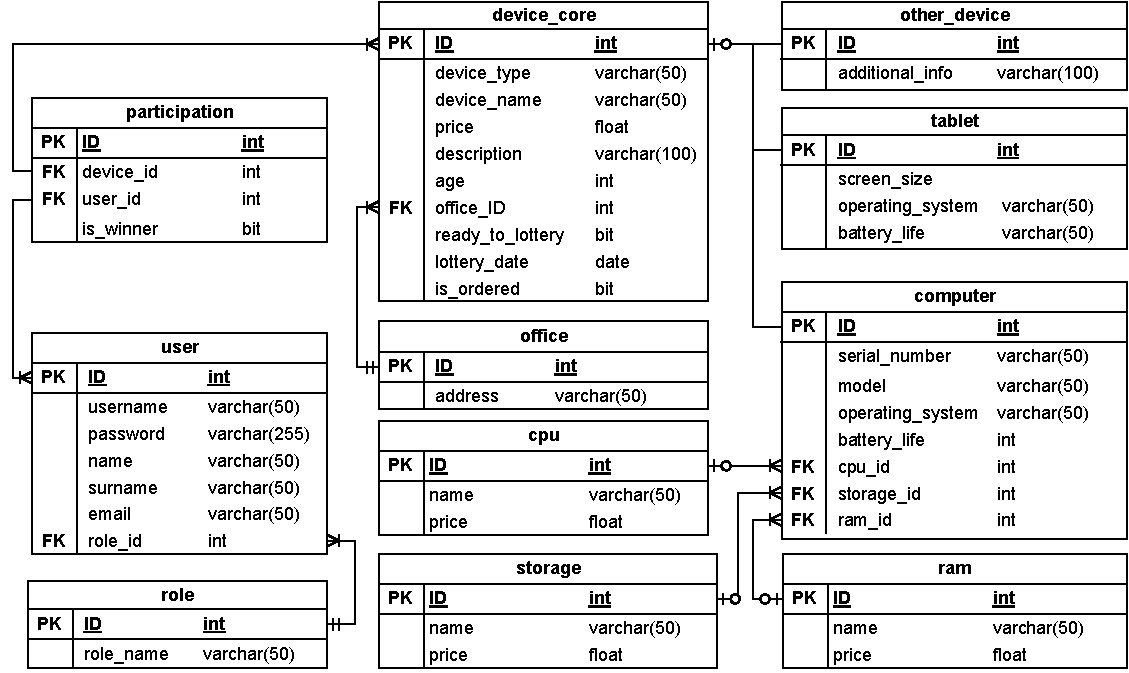
\includegraphics[width=\linewidth]{rys04/ER_Diagram.pdf}
    \caption{Diagram związków encji}
    \label{ErDiagram_etykieta}
\end{figure}

\section{Tworzenie bazy danych}
W tworzeniu baz danych istnieją dwa podejścia: code first i database first. W implementacji systemu wykorzystane zostało podejście database first. Daje do w początkowym etapie projektowania większą przejrzystość danych. Po stworzeniu modelu można potem skorzystać z gotowych narzędzi które pozwolą automatycznie wygenerować kod odzwierciedlający model danych.

Przy tworzeniu bazy danych wykorzystywanym narzędziem jest SSMS \ref{ssms:label}. 
Na początek stworzono tabele na podstawie diagramu związków encji \ref{ErDiagram_etykieta} oraz określono jej relacje. Przykład tworzenia encji oraz jej relacji znajduje się na poniższych rysunkach.

\begin{figure}[htb]
  \centering
	\begin{tabular}{@{}ll@{}}
	a) & b) \\
  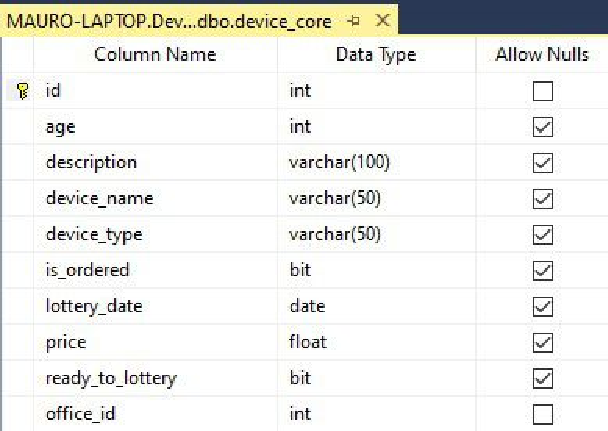
\includegraphics[width=0.475\textwidth]{rys04/design.pdf} & 
	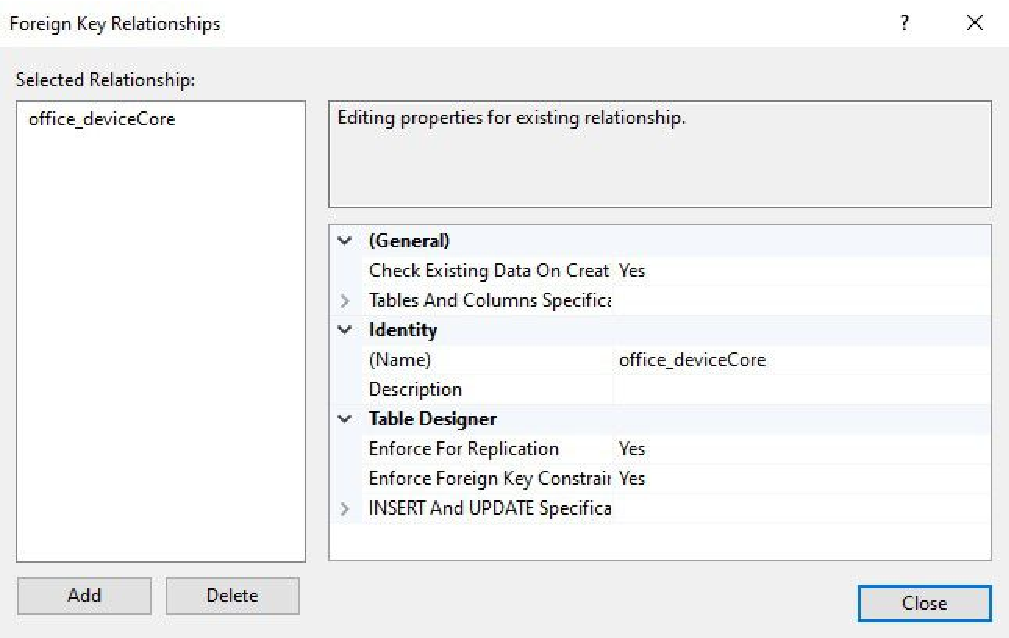
\includegraphics[width=0.475\textwidth]{rys04/relation.pdf}
	\end{tabular}
  \caption{Tworzenie bazy danych SSMS a) model, b) definiowanie relacji}
  \label{ssms_tworzenie:label}
\end{figure}

Po stworzeniu wszystkich tabel możliwe jest wygenerowanie kodu. Wykorzystano do tego plugin JPA Buddy oraz wbudowane narzędzia Intelij. Upraszcza to proces implementacji systemu. Ponizej przedstawiono sposób generowania kodu encji dla klasy computer.

\begin{figure}[h]
		\centering
    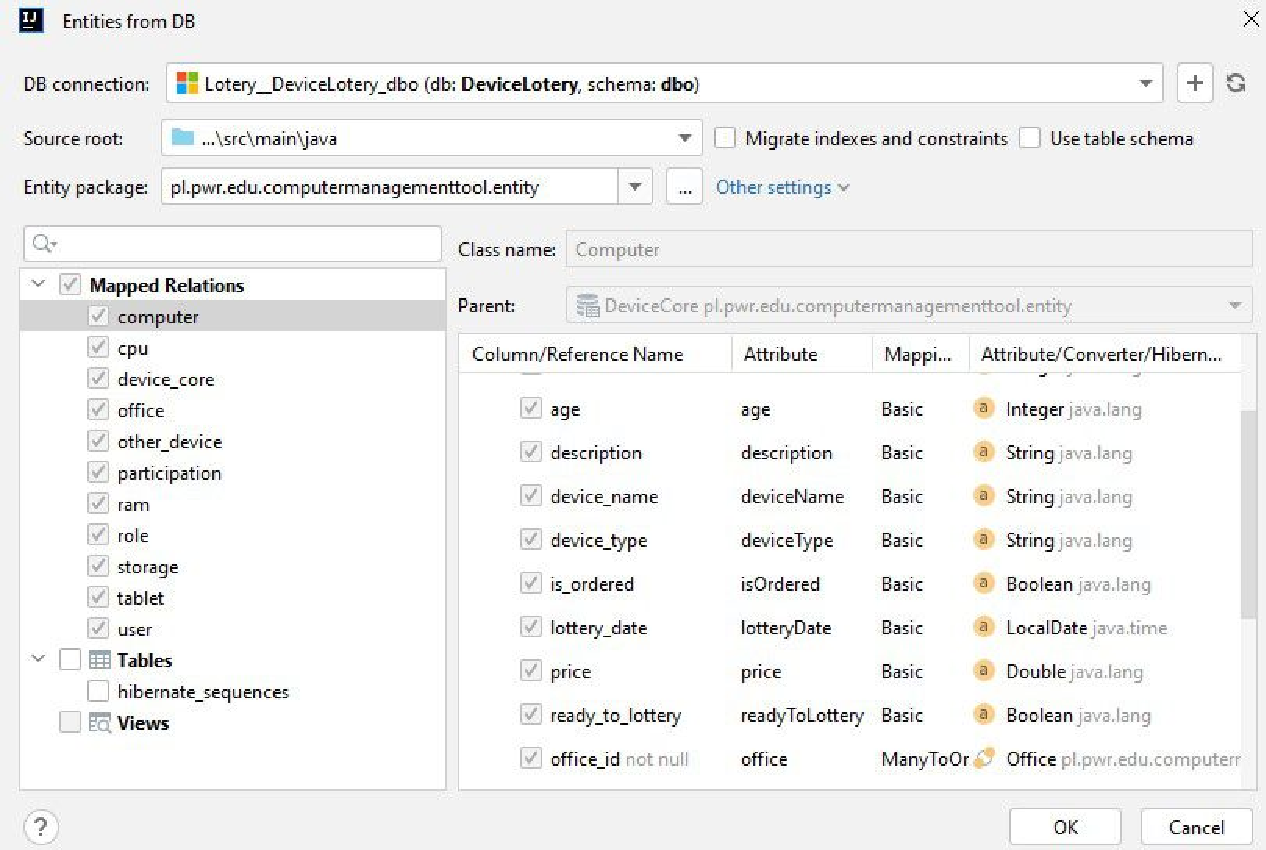
\includegraphics[width=0.7\linewidth]{rys04/generate.pdf}
    \caption{Generowaniu kodu na podstawie tabeli computer przy użyciu Intelij Idea}
    \label{generate:label}
\end{figure}

Tworzenie w ten sposób początkowej struktury projektu jest bardzo pomocne. Jednak kiedy definiuje się sposób dziedziczenia tabel to jedynym sposobem jest zdefiniowanie relacji wykorzystując Hibernate. O sposobie dziedziczenia tabel przez Hibernate napisano na początku tego rozdziału \ref{dzedziczenie_hibernate:label} Szczegóły implementacji dotyczące klasy device\_core opisano w podrozdziale \ref{entity_deviceCore}. Odpowiednia konfiguracja projektu umożliwia aktualizowanie struktury bazy danych. Możliwe dzięki temu jest wyeliminowanie nadmiarowego kodu oraz skorzystanie abstrakcji dostarczanej przez dziedziczenie. Gdy Hibernate zaktualizuje strukture bazy danych w SSMS automatycznie powstają odpowiednie tabele i relacje klas sprzętu. Zarządzanie unikalnością kluczy dla tych klas też jest możliwa tylko z poziomu kodu.
 

\chapter{Implementacja}

\section{Architektura}


\subsection{Struktura interfejsu REST}
% TO DO: Opis do poprawy (bo zmieniono układ tabel)
Poniższa tabela \ref{tab:rest1} prezentuje jakie zapytania mogą być odbierane przez aplikację serwerową. Z racji tego, że w aplikacji wykorzystywane są typy generyczne w klasach kontrolerach urządzeń i komponentów komputera (implementacja \ref{controller_genericDevice} uproszczono tabele by pokazać ogólną formę zapytań. Wszystkie zapytania posiadające "`devices"' w ścieżce umożliwiają alternatywne wywołanie zapytania na podstawie typu sprzętu. Ogólna zasada jest taka aby zastąpić "`devices"' odpowiadającemu typowi sprzętu: "`computers"', "`tablets"', "`other-devices"'. Powoduje to, że zapytanie wykonywane jest przez kontroler tej klasy, a co za tym idzie ma określony typ. Możliwe jest też wykonanie zapytania nie zmieniając ścieżki. Wtedy takie zapytanie wykonywane jest na ogólnym rodzaju sprzętu. Przykładowo "`devices/all"' pobiera wszystkie sprzęty nie zwracając uwagi na typ, natomiast "`computers/all"' pobiera tylko sprzętu typu "`Computer"'. Podobne rozwiązanie wykorzystano w komponentach komputera. Dotyczy to zapytań mających w ścieżce: "`component"'. Tutaj należy zamienić "`component"' na jeden z trzech dostępnych typów komponentu: "`rams"', "`cpus"', "`storages"'. W tym wypadku nie ma możliwości wywołania zapytania zawierającego "`component"'.

\begin{table}[H]\small
	\centering
\caption{Tabela prezentująca strukturę REST (cz.1)}
\label{tab:rest1}
\begin{tabularx}{\linewidth}{|X|l|p{3cm}|X|}
    \hline
    Ścieżka & Metoda & Parametry & Opis  \\
    \hline \hline
		/devices/all 	& GET & - & Pobranie danych sprzętów na podstawie określonego typu \\
		\hline
		/devices/{id} & GET & id urządzenia 	& Pobranie danych wszystkich sprzętów\\
    \hline
		/devices/{id}	& DELETE & id urządzenia 	& Usunięcie sprzętu\\
    \hline
		 /computers/update/id & PATCH & id sprzętu oraz zmienione dane sprzętu& aktualizacja danych komputera\\
		\hline
		 /tablets/update/id & PATCH & id sprzętu oraz zmienione dane sprzętu& aktualizacja danych tabletu\\
		\hline	 
		/other-device/update/id & PATCH & id sprzętu i zmienione dane sprzętu & aktualizacja danych innego urządzenia\\
		\hline
			 /computers/add & POST	& dane komputera 	& Dodanie nowego komputera	\\
    \hline
		/tablets/add & POST	& dane tabletu & Dodanie nowego urządzenia	\\
    \hline
		/other-device/add & POST	& dane innego urządzenia 	& Dodanie nowego urządzenia	\\
    \hline
		/devices/by-office& GET	& id biura 	& Pobranie danych sprzętu znajdujących się w biurze\\
    \hline
		/devices/all-ready-to-lottery& GET	& - & Pobranie danych sprzętów które są gotowe do losowania\\
    \hline
		
		/devices/all-ready-to-lottery-by-officeId/id& GET	& id biura & Pobranie danych sprzętów które są gotowe do losowania i znajdują się w danym biurze\\
    \hline
		/devices/set-ready-to-lottery/id 		& PUT	& id sprzętu & Ustawienie gotowości sprzętu do losowania	\\
    \hline
		/devices/set-not-ready-to-lottery/id & PUT	& id sprzętu & Ustawienie braku gotowości sprzętu do losowania	\\
    \hline
		/devices/set-ordered/id & PUT	& id sprzętu & Ustawienie statusu sprzętu na dostarczone	do pracownika	\\
    \hline
		/devices/set-not-ordered/id & PUT	& id sprzętu & Ustawienie statusu sprzętu na dostarczone	do pracownika	\\
    \hline
		/components/all 	& GET & - & Pobranie danych wszystkich procesorów, ram lub dysków pamięci \\
		\hline
		/components/{id} & GET & id komponentu 	& Pobranie danych procesora, ram lub dysku pamięci\\
    \hline
		/components/{id}	& DELETE & id komponentu 	& Usunięcie procesora, ram lub dysku pamięci\\
    \hline
		 /components/update/id & PUT & id sprzętu oraz zmienione dane sprzętu& aktualizacja danych komputera\\
		\hline
		 /offices/all	& GET & - & Pobranie wszystkich biur w systemie\\
		\hline
		/users/all	& GET & - & Pobranie wszystkich użytkowników w systemie\\
		\hline
		\end{tabularx}
		\end{table}

\begin{table}[H] \small
	\centering
\caption{Tabela prezentująca strukturę REST (cz.2)}
\label{tab:rest2}	 
\begin{tabularx}{\linewidth}{|X|l|p{3cm}|X|}\hline
    Ścieżka & Metoda & Parametry & Opis  \\
    \hline \hline
		 /users/all-standard	& GET & -& Pobranie wszystkich użytkowników z rolą pracownik w systemie\\
		\hline
		 /users/id & GET & - & Pobranie użytkownika\\
		\hline
		 /users/id & DELETE & - & Usunięcie użytkownika\\
		\hline
		 /participation/add & POST & id użytkownika oraz id urządzenia & Dodanie uczestnictwa użytkownika w loterii do wybranego sprzętu\\
		\hline
		 /participation/all& POST & - & Wyświetlenie wszystkich uczestników dla każdego sprzętu\\
		\hline
		 /participation/id & DELETE & - & Usunięcie uczestnictwa o zadanym id\\
		\hline
		 /participation/delete-by-user\_id-and-device\_id& DELETE & id użytkownika i id sprzętu & Usunięcie uczestnictwa spełniającego zadane kryteria\\
		\hline
		 /participation/all-wins& GET & - & Wyświetlenie wszystkich zwycięskich uczestników\\
		\hline
		 /participation/user-lottery-history/id & GET& id użytkownika & Wyświetlenie historii uczestnictwa użytkownika o zadanym id\\
		\hline
		 /participation/user-win-history/id & GET& id użytkownika & Wyświetlenie historii zwycięstw użytkownika o zadanym id\\
		\hline
		 /participation/user-lose-history/id & GET& id użytkownika & Wyświetlenie historii porażek użytkownika o zadanym id\\
		\hline
		 /participation/user-pending-lottery/id & GET& id użytkownika & Wyświetlenie uczestnictwa które czeka na losowanie\\
		\hline
		 /participation/device-participation/id& GET& id urządzenia & Wyświetlenie wszystkich użytkowników zapisanych na losowaniu urządzenia o zadanym id\\
		\hline
		 /participation/check-if-user-in-lottery& GET& id urządzenia oraz id użytkownika& Sprawdzenie czy użytkownik bierze udział w losowaniu\\
		\hline
		 /participation/select-random-winner/id& GET& id urządzenia& Losowanie zwycięzcy loterii dla urządzenia o zadanym id\\
		\hline
\end{tabularx}
\end{table}



\section{Aplikacja serwerowa}
Do zarządzania danymi wykorzystywana jest aplikacja serwerowa. Przetwarza ona żądania aplikacji klienckiej. Dostarcza ona funkcjonalność uwierzytelniania i autoryzacji. W wyniku zapytań wysłanych przez aplikację kliencką wyświetlane są w aplikacji odpowiednie dane. Możliwe jest też dodawanie i usuwanie odpowiednich rekordów. Implementacja odbywa się z wykorzystywaniem języka Java z frameworkami Spring oraz Hibernate \ref{tab:zestawienie_narzędzi} Graficzną reprezentacje struktury projektu aplikacji serwerowej pokazano na rysunku \ref{backend_struktura:label}

\subsection{Struktura projektu}
Ścieżka pakietowa wykorzystana jest odwróconą ścieżką domenową Politechniki Wrocławskiej oraz nazwy projektu: pl.edu.pwr.computermanagamenttool. Następnie pakiety które są dołączone do tej ścieżki odpowiadają funkcjom które pełnią klasy. Wyróżnia się tutaj pakiety:
\begin{itemize}
\item pl.edu.pwr.computermanagementtool - pakiet ogólny przechowywujący pozostałe pakiety. Klasa ComputerManagementToolApplication posiada metodę Main odpowiedzialną za uruchomienie aplikacji. Klasa JacksonConfig jest konfiguracją odpowiedzialną za serializacje formatu JSON. Natomiast klasa PasswordEncoderUtil jest odpowiedzialna za szyfrowanie haseł użytkowników korzystających z systemu.
\item controller - pakiet przechowujący w sobie klasy kontrolerów odpowiedzialne za wykonywanie zapytań aplikacji za pomocą interfejsu REST
\item dto - pakiet który jest odpowiedzialny za przechowywanie klas służących do przechowywania danych i ułatwiania ich przesyłania między różnymi częściami systemu. Wykorzystywany jest w klasach kontrolera.
\item entity - pakiet przechowujący definicje encji reprezentowanych w bazie danych
\item repository - pakiet przechowujący repozytoria służące do komunikacji z bazą danych.
\item service - pakiet przechowujący serwisy które są odpowiedzialne za warstwę logiki biznesowej w systemie
\end{itemize}


\begin{figure}[htb]
  \centering
	\begin{tabular}{@{}lll@{}}
	a) & b) & c) \\
  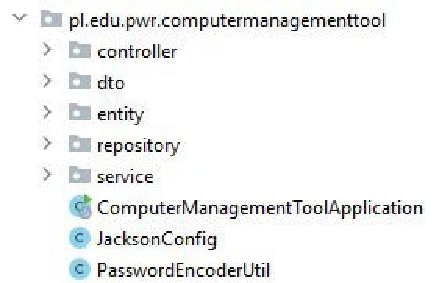
\includegraphics[width=0.3\textwidth]{rys05/backend/ogolne.pdf} & 
	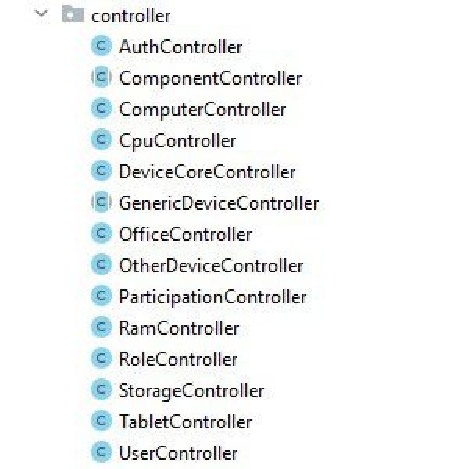
\includegraphics[width=0.3\textwidth]{rys05/backend/controller.pdf} &
	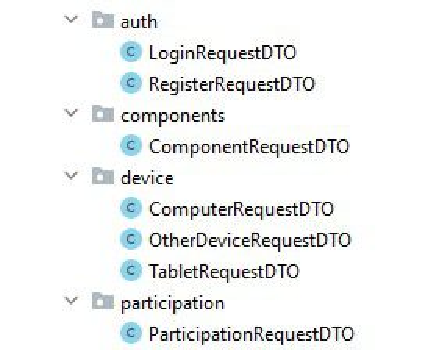
\includegraphics[width=0.3\textwidth]{rys05/backend/dto.pdf} \\

	d) & e) & f) \\
	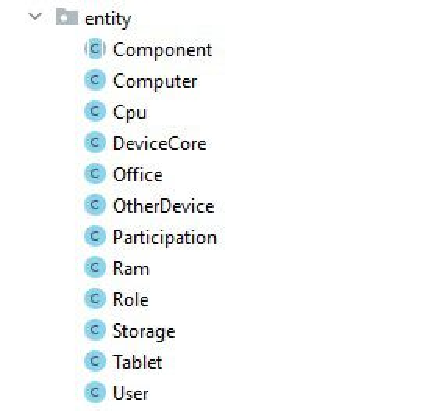
\includegraphics[width=0.3\textwidth]{rys05/backend/entity.pdf} &
	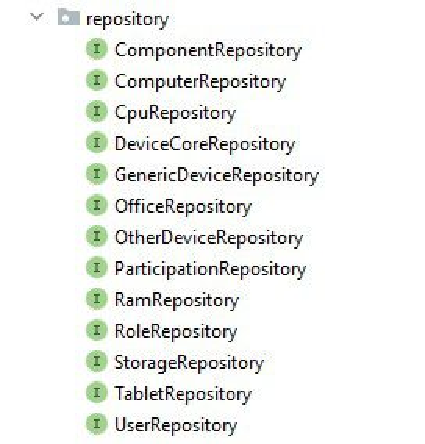
\includegraphics[width=0.3\textwidth]{rys05/backend/repository.pdf} &
	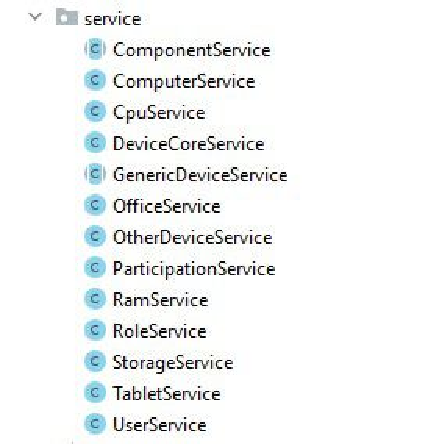
\includegraphics[width=0.3\textwidth]{rys05/backend/service.pdf}
	\end{tabular}
  \caption{Struktura projektu a) ogólna struktura, b) kontrolery, c) data transfer object, d) encje, e) repozytoria, f) serwisy}
  \label{backend_struktura:label}
\end{figure}

\newpage
\subsection{Fragmenty implementacji}
\subsubsection {Fragment kodu klas encji wykorzystującej schemat dziedziczenia}

\begin{lstlisting}[language=Java, style=JavaStyle, caption={Klasa nadrzędna reprezentująca rdzeń sprzętu: DeviceCore}, label={entity_deviceCore}]
@Entity
@Table(name = "device_core")
@Inheritance(strategy = InheritanceType.TABLE_PER_CLASS)
public class DeviceCore {
    @Id
    @GeneratedValue(strategy = GenerationType.TABLE)
    @Column(name = "id", nullable = false)
    private Integer id;

    @Column(name = "device_type", length = 50)
    private String deviceType;

    @Column(name = "device_name", length = 50)
    private String deviceName;
		
		// Pozostała część klasy

\end{lstlisting}
W linii 3 listingu klasy DeviceCore \ref{entity_deviceCore} określono schemat dziedziczenia TABLE\_PER\_CLASS. O sposobie dziedziczenia napisano w podrozdziale \ref{dzedziczenie_hibernate:label}. Linia 3 określa strategie generowania klucza. Hibernate tworzy wtedy specjalną tabelę w bazie danych która odpowiedzialna jest za przechowywanie unikalnych kluczy głownych dla encji sprzętu w aplikacji. W listingu kodu \ref{entity_computer} nie trzeba wtedy definować klucza.

\begin{lstlisting}[language=Java, style=JavaStyle,  caption={Klasa potomna: Computer, reprezentująca komputer}, label={entity_computer}]
@Entity
@Table(name = "computer")
public class Computer extends DeviceCore{

    public static final String DEVICE_TYPE = "COMPUTER";
    @Column(name = "serial_number", length = 50)
    private String serialNumber;

    @Column(name = "operating_system", length = 50)
    private String operatingSystem;

    @Column(name = "battery_life", length = 50)
    private String batteryLife;
		
		// Pozostała część klasy
\end{lstlisting}
W linii 3 określone zostało dziedziczenie po klasie nadrzędnej reprezentującej rdzeń sprzętu. Pola które należy określić w tej klasie są unikalnymi polami tabeli computer. W linii 4 istnieje statyczna zmienna DEVICE\_TYPE która pomaga określić jakiego rodzaju dany sprzęt. Wykorzystywane jest to w aplikacji klienckiej.


\subsubsection{Przykład kodu repozytorium dla urządzeń dziedziczącym po rdzeniu sprzętu}
Repozytorium sprzętu komputerowego zostało napisane z użyciem wyrażeń generycznych. Wykorzystanie ich przyczynia się do uproszczenia kodu oraz łatwiejszej jego rozbudowy.

\begin{lstlisting}[language=Java, style=JavaStyle,  caption={Generyczne repozytorium sprzętu komputerowego:  GenericDeviceRepository}, label={repo_genericDevice}]
@NoRepositoryBean
public interface GenericDeviceRepository<T extends DeviceCore> extends JpaRepository<T, Integer> {
    
    List<T> findAllByReadyToLotteryIsTrue();
    List<T> findAllByOfficeId(int officeId);
}
\end{lstlisting}

W lini 1 adnotacja @NoRepositoryBean jest używana do oznaczenia interfejsów które nie mają mieć swojej instancji. Oznacza to, że nie jest on przeznaczony do utworzenia instancji repozytorium w trakcie uruchomiania aplikacji. W linii 4 i 5 poprzez zdefiniowanie metody możliwe jest wykonanie konkretego zapytania SQL do bazy danych. Z racji, że klasy sprzętu komputerowego mają zbliżone funkcjonalności nie trzeba dostarczać tych samych interfejsów we wszystkich repozytoriach tylko zastosować schemat dziedziczenia.

\subsubsection{Fragmenty implementacji klasy kontrolerów sprzętu}

\begin{lstlisting}[language=Java, style=JavaStyle,  caption={Klasa nadrzędna kontrolera sprzętu: GenericDeviceController}, label={controller_genericDevice}]
public abstract class GenericDeviceController<T extends DeviceCore> {

    protected final GenericDeviceService<T> genericDeviceService;
    protected final GenericDeviceRepository<T> genericRepository;

    protected GenericDeviceController(GenericDeviceService<T> genericDeviceService, GenericDeviceRepository<T> genericRepository) {
        this.genericDeviceService = genericDeviceService;
        this.genericRepository = genericRepository;
    }

    @GetMapping("/{id}")
    @CrossOrigin(origins = "*")
    T getOneBasicDevice(@PathVariable int id){
        return genericDeviceService.getDeviceById(id);
    }

    @GetMapping("/all")
    @CrossOrigin(origins = "*")
    List<T> getAllBasicDevices(){
        return genericDeviceService.getAllDevices();
    }

    @GetMapping("/all-ready-to-lottery")
    @CrossOrigin(origins = "*")
    List<T> getAllReadyToLotteryDevice(){
        return genericDeviceService.getAllReadyToLotteryDevices();
    }
		
		// Pozostała część klasy
		
		@PutMapping("/set-ready-to-lottery/{id}")
    @CrossOrigin(origins = "*")
    public ResponseEntity<T> setReadyToLottery(@PathVariable int id){
        try{
            T updatedBasicDevice = genericDeviceService.setReadyToLottery(id);
            return new ResponseEntity<>(updatedBasicDevice, HttpStatus.OK);
        } catch (RuntimeException e){
            return new ResponseEntity<>(HttpStatus.NOT_FOUND);
        }
    }
		
		// Pozostała część klasy
		
\end{lstlisting}

Kontrolery pełnią istotną funkcje w systemie. Umożliwiają one definiowanie zapytań REST które będą wysyłane do serwera. Wykorzystując abstrakcje oraz wyrażenia generyczne możliwe jest wykonanie niektórych requestów bez konieczności ich implementacji w klasach potomnych.


\begin{lstlisting}[language=Java, style=JavaStyle,  caption={Klasa potomna reprezentująca ogólną postać sprzętu}, label={controller_device}]
@RestController
@RequestMapping("/devices")
public class DeviceCoreController extends GenericDeviceController<DeviceCore>{

    protected DeviceCoreController(DeviceCoreService deviceCoreService, GenericDeviceRepository<DeviceCore> genericRepository) {
        super(deviceCoreService, genericRepository);
    }
}
\end{lstlisting}

Powyższa klasa w listingu kodu \ref{controller_device} nie posiada własnych metod. Umożliwia jednak wykonywanie ogólnych operacji dotyczących sprzętu. Możliwe jest między innymi pobranie informacji dotyczące sprzętu bez względu na jego typ co idealanie obrazuje test **referencja do zapytania w postmanie**


\subsubsection{Fragmenty implementacji klas serwisów sprzętu}


\begin{lstlisting}[language=Java, style=JavaStyle,  caption={Klasa nadrzędna serwisu sprzętu GenericDeviceService}, label={service_tablet}]

public abstract class GenericDeviceService<T extends DeviceCore> {

    protected final GenericDeviceRepository<T> genericDeviceRepository;
    protected final OfficeRepository officeRepository;

    public GenericDeviceService(GenericDeviceRepository<T> genericRepository, OfficeRepository officeRepository) {
        this.genericDeviceRepository = genericRepository;
        this.officeRepository = officeRepository;
    }

    public T getDeviceById(int id) {
        Optional<T> basicDeviceOptional = genericDeviceRepository.findById(id);
        return basicDeviceOptional.orElseThrow(()-> new RuntimeException("Device not found with id: " + id));
    }

    public List<T> getAllDevices() {
        return genericDeviceRepository.findAll();
    }
		// Pozostała część klasy

protected DeviceCore addDevice(Class<? extends DeviceCore> deviceClass, String deviceName, Double price, String description, Integer age, Boolean readyToSell, Integer officeId) {

        if(officeId == null){
            throw new RuntimeException("Office required");
        }
        Optional<Office> officeOptional = officeRepository.findById(officeId);
        Office office = officeOptional.orElseThrow(() -> new RuntimeException("Office not found with id: " + officeId));

        DeviceCore deviceCore;
        try {
            deviceCore = deviceClass.getDeclaredConstructor().newInstance();
        } catch (InstantiationException | IllegalAccessException | NoSuchMethodException | InvocationTargetException e) {
            throw new RuntimeException("Error creating device", e);
        }

        deviceCore.setDeviceName(deviceName);
        deviceCore.setPrice(price);
        deviceCore.setDescription(description);
        deviceCore.setAge(age);
        deviceCore.setReadyToSell(readyToSell);
        deviceCore.setOffice(office);

        return deviceCore;
    }
		
		// Pozostała część klasy

\end{lstlisting}
Serwisy są odpowiedzialne za warstwe logiki biznesowej systemu. W linii 12 widnieje metoda która pozwala na pobranie sprzętu. W linii 17 natomiast jest możliwe pobranie wszystkich sprzętów. Odbywa się to przy pomocy parametryzowanych typów danych T. Metoda zdefiniowana w linii 22 pozwala uprościć dodawanie sprzętu, implementując część logiki ustawiając parametry charakterystyczne dla rdzenia sprzętu. Jednak aby utworzyć odpowiedni typ niezbędne jest określenie jakiego typu będzie dodawane urządzenie, Dlatego w linii 22 metoda jako parametr przyjmuje Class<? extends DeviceCore> który oznacza typ aplikacji. Tak zdefiniowana metoda może zostać użyta do dodania sprzętu w kalsach potomnych co pokazano w listingu \ref{service_tablet}

\begin{lstlisting}[language=Java, style=JavaStyle,  caption={Klasa potomna serwisu tabletu: TabletService }, label={service_tablet}]

@Service
public class TabletService extends GenericDeviceService<Tablet>{

    public TabletService(TabletRepository tabletRepository, OfficeRepository officeRepository){
        super(tabletRepository, officeRepository);
    }

    public Tablet addTablet(String deviceName, Double price, String description,
                            Integer age, String officeAddress,
                            String screenSize, String operatingSystem, String batteryLife){

        Tablet tablet = (Tablet) addDevice(Tablet.class, deviceName, price, description,
                                                                age, officeAddress);

        tablet.setScreenSize(screenSize);
        tablet.setOperatingSystem(operatingSystem);
        tablet.setDeviceType(Tablet.DEVICE_TYPE);
        tablet.setBatteryLife(batteryLife);

        return genericDeviceRepository.save(tablet);
    }
		// Pozostała część klasy
\end{lstlisting}

Serwis klasy TabletService dziedziczy i parametryzuje metody klasy GenericDeviceService. Wykorzystuje on w linii 13 metodę klasy nadrzędnej co uprasza implementacje metody dodającej sprzęt(linia 9)



\section {Aplikacja kliencka}
Aplikacja kliencka jest aplikacją internetową dostarczającą przyjazny interfejs użytkownika. W aplikacji klienckiej napisanej w języku JavaScript z wykorzystaniem biblioteki React (tabela \ref{tab:zestawienie_narzędzi}) istnieją zdefiniowane zapytania REST do aplikacji serwerowej. Wykorzystując te zapytania na widoku widocznym dla użytkownika zostają podjęte specjalne akcje które ten widok aktualizują. Formularze pokazywane są w takiej formie, że po kliknięciu odpowiedniego przycisku ukazuje się formularz na danym widoku. Zestawienie widoków, ścieżek i roli pokazano w tabeli \ref{tab:zestawienie_widokow}

\subsection{Struktura projektu}
Ogólna struktura projektu została stworzona przez wywołanie komendy tworzącej aplikacje Reacta: npx create-react-app frontend. Następnie utworzono folder components który w sobie zawiera foldery przechowujące pliki JavaScript na podstawie pełnionych funkcji w projekcie. Foldery i odpowiadające im funkcje: 
\begin {itemize}
\item \textbf{auth} przechowuje pliki odpowiedzialne za obsługę i stylizacje widoków logowania i rejestracji
	\begin{itemize}
	\item Login.js - skrypt odpowiedzialny za widok i funkcjonalność logowania
	\item Register.js - skrypt odpowiedzialny za widok i funkcjonalność rejestracji
	\item Login.css - arkusz styli odpowiedzialny za stylizacje widoków logowania i rejestracji
	\end{itemize}
\item \textbf{bar} przechowuje skrypty odpowiedzialne za paski nawigacyjne poszczególnych widoków.
	\begin{itemize}
	\item AdminHomeBar.js - skrypt odpowiedzialny za pasek nawigacyjny na widoku domowym administratora: Home.js
	\item ComputerComponentsBar.js -skrypt odpowiedzialny za pasek nawigacyjny dla widoku komponentów: ComputerComponents.js
	\item ManageUserBar.js -skrypt odpowiedzialny za pasek nawigacyjny widoku zarządzania użytkownikami: Users.js
	\item UserHomeBar.js - skrypt odpowiedzialny za pasek nawigacyjny na widoku domowym pracownika: Home.js
	\item UserLotteryHistory -skrypt odpowiedzialny za pasek nawigacyjnym na widoku historii loterii użytkownika: UserLotteryHistory.js
	\item UsersInLottery.js -skrypt odpowiedzialny za pasek nawigacyjny na widoku użytkowników biorących udział w loterii: UsersInLottery.js
	\end{itemize}
\item \textbf{computer\_components} przechowuje skrypty formularzy komponentów komputera które mogą dodawać lub modyfikować te komponenty
	\begin{itemize}
	\item CpuForm.js - formularz procesora
	\item RamForm.js - formularz pamięci RAM
	\item StorageForm.js - formularz pamięcu dyskowej
	\end{itemize}
\item \textbf{device\_form} przechowuje skrypty oraz arkusz styli odpowiedzialne za logikę formularzy dodawania, modyfikacji urządzeń
	\begin{itemize}
	\item AddNewFormPopup.js - formularz umożliwiający wybór formularza który dodaje komputer, tablet, lub inne urządzenie
	\item ComputerForm.js -formularz komputera
	\item DeviceForm.css - arkusz styli odpowiedzialny za stylizacje formularzy
	\item FormPopup.js - skrypt odpowiedzialny za logikę i wybór rodzaju formularza(dodawanie, modyfikacja, informacje) urządzenia.
	\item OtherDeviceForm - formularz innego urządzenia
	\item TabletForm.js - formularz tabletu
	\end{itemize}
\item \textbf{view} przechowuje w sobie skrypty oraz arkusz styli odpowiedzialne za widoki aplikacji
	\begin{itemize}
	\item ComputerComponets.js -widok dostępny tylko dla administratora. Zawiera w sobie informacje o komponentach komputera w postaci tabeli
	\item Home.css - arkusz styli odpowiedzialny za stylizacje widoków
	\item Home.js - widok strony domowej, ma w sobie dwa warianty: Administartora i Pracownika
	\item UserLotteryHistory.js - widok hostorii loterii użytkownika o zadanym ID. Dostępny dla pracownika i administratora.
	\item Users.js - widok pracowników zarejestrowanych w systemie. Dostępny tylko dla administratora
	\item UsersInLottery - widok pracowników biorących udział w loterii danego sprzętu. Dostępny tylko dal administratora.
	\end{itemize}
\end{itemize}

Równolegle do folderu components w folderze src istnieją jeszcze dwa skrypty które są niezbędne do funkcjonowania aplikacji.
\begin{itemize}
	\item App.js zawiera w sobie scieżki url pod którymi dostępne są poszczególne widoki
	\item index.js - funkcja główna programu
\end{itemize}

Strukturę projektu pokazano na Rysunku \ref{frontend_struktura:label}


\begin{table}[htb] \small
	\centering
\caption{Zestawienie ścieżek url dostępnych w aplikacji klienckiej}
\label{tab:zestawienie_widokow}
\begin{tabularx}{\linewidth}{|X|X|X|X|}
    \hline
    Ścieżka & Widok & Skrypt & Rola\\
    \hline \hline
    /auth/login & Logowanie &  Login.js & Przed nadaniem roli\\
    \hline
    /auth/register & Rejestracja & Register.js & Przed nadaniem roli\\
    \hline
    /home & Strona domowa z tabelą sprzętów & Home.js & Administrator lub Pracownik\\
    \hline
    /users & Tabela pracowników & Users.js & Administrator\\
    \hline
		/components & Tabela komponentów komputera& ComputerComponents.js & Administrator\\
    \hline
		/users-in-lottery & Tabela użytkowników biorących udział w loterii& UsersInLottery.js & Administrator lub Pracownik\\
    \hline
		/users-lottery-history & Tabela zawierająca historię loteri & UsersLotteryHistory.js & Administatro lub Pracownik\\

    \hline
\end{tabularx}
\end{table}


\begin{figure}[htb]
  \centering
	\begin{tabular}{@{}lll@{}}
	a) & b) & c) \\
  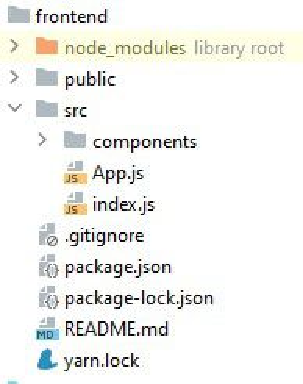
\includegraphics[width=0.3\textwidth]{rys05/frontend/frontend.pdf} & 
	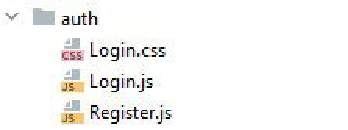
\includegraphics[width=0.3\textwidth]{rys05/frontend/auth.pdf} &
	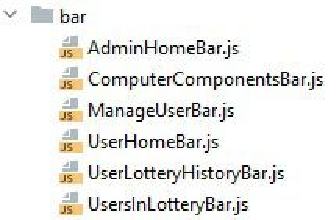
\includegraphics[width=0.3\textwidth]{rys05/frontend/bar.pdf} \\

	d) & e) & f) \\
	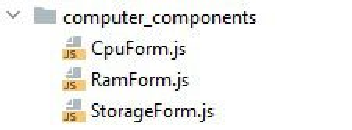
\includegraphics[width=0.3\textwidth]{rys05/frontend/components.pdf} &
	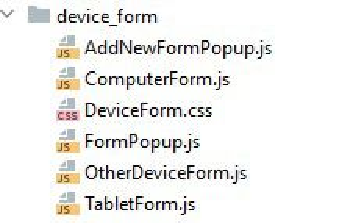
\includegraphics[width=0.3\textwidth]{rys05/frontend/deviceform.pdf} &
	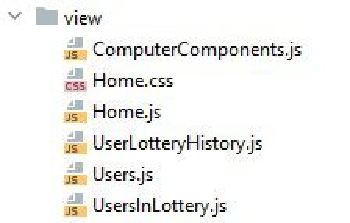
\includegraphics[width=0.3\textwidth]{rys05/frontend/view.pdf}
	\end{tabular}
  \caption{Struktura projektu a) ogólna struktura, b) Logowanie i rejestracja, c) pasek nawigacyjny, d) formularze komponentów, e) formularze sprzętów, f) widoki stron}
  \label{frontend_struktura:label}
\end{figure}



\subsection{Fragmenty implementacji}
	\subsubsection{Ścieżki url dla widoków aplikacji}
	

\begin{lstlisting}[language=JavaScript, style=JavaScriptStyle,  caption={Zdefiniowane ścieżki url widoków systemu }, label={app_frontend:label}]
	
	const App = () => {
    return (
        <Router>
            <Routes>
                <Route path="/auth/login" element={<Login />} />
                <Route path="/auth/register" element={<Register />} />
                <Route path="/home" element={<Home />} />
                <Route path="/" element={<Navigate to="/auth/login" />} />
                <Route path="/auth/*" element={<Navigate to="/auth/login" />} />
                <Route path="/users" element={<Users/>}/>
                <Route path="/components" element={<ComputerComponents/>}/>
                <Route path="/users-in-lottery" element={<UsersInLottery/>}/>
                <Route path="/user-lottery-history" element={<UserLotteryHistory/>}/>
            </Routes>
        </Router>
    );
};
	
\end{lstlisting}
Powyższy listing kodu \ref{app_frontend:label} definiuje ścieżki url pod którymi dostępne są poszczególne widoki~\ref{tab:zestawienie_widokow}


\subsubsection{Sparametryzowany formularz urządzenia}

\begin{lstlisting}[language=JavaScript, style=JavaScriptStyle,  caption={Obsługa formularzy}, label={render_data:label}]

function FormPopup(props){
    
 const {setTrigger, formType, deviceType, deviceId} = props;
    
  return (props.trigger) ? (
    <div className="popup">
      <div>
         {deviceType === 'COMPUTER' && <ComputerForm setTrigger={props.setTrigger} formType={formType} deviceId={deviceId}/>}
         {deviceType === 'TABLET' && <TabletForm setTrigger={props.setTrigger} formType={formType} deviceId={deviceId}/>}
         {deviceType === 'OTHER' && <OtherDeviceForm setTrigger={props.setTrigger}  formType={formType} deviceId={deviceId} />}
         {props.children}
      </div>
    </div>
 ) : "";
}

export default FormPopup
										
\end{lstlisting}

Powyższy listing kodu \ref{render_data:label} dla skryptu FormPopup.js  służy do dodawania różnych rodzajów formularza sprzętów z różnymi wariantami. Przyjmuje 4 argumenty. Przekazywanie tych parametrów odbywa się w linii 4 z wykorzystaniem "`props"'. Zmienna deviceType odpowiada dla jakiego urządzenia dotyczy formularz. Może on dotyczyć komputera, tableta lub innego urządzenia co pokazano w liniach 9-11. Zmienna setTrigger jest odpowiedzialna za to czy formularz jest aktualnie wyświetlany nad widokiem. Zmienna formType dotyczy wariant formularza. Istnieją 3 warianty jednego formularza i dotyczą one kolejno: dodawania nowego sprzętu, modyfikacji sprzętu oraz wyświetlania informacji o sprzęcie. Warianty formularza pokazano rysunku **referencja do rysunku**. Tak stworzona funkcja umożliwia zarządzanie formularzami które zostały zdefiniowane w plikach ComputerForm.js, TabletForm.js oraz OtherDeviceForm.js.

\begin{lstlisting}[language=JavaScript, style=JavaScriptStyle,  caption={Przykładowe zapytanie do serwera dla formularza komputera}, label={addComputer:label}]

const handleAddComputer = async (e) =>{

        try{
            const compData ={
                "deviceName" : formData.deviceName,
                "price" : formData.price,
                "description" : formData.description,
                "age" : formData.age,
                "officeAddress" : formData.office,
                "serialNumber" : formData.serialNumber,
                "model" : formData.model,
                "operatingSystem" : formData.model,
                "batteryLife" : formData.batteryLife,
                "cpuName" : formData.cpu,
                "storageName" : formData.storage,
                "ramName" : formData.ram
            };

            const response = await axios.post('http://localhost:8080/computers/add', compData, {

            });

        }catch (error){
            console.error('Bład dodawania komputera', error)
        }

\end{lstlisting}

Powyższy listing kodu \ref{addComputer:label} ukazuje w jaki sposób aplikacje kliencka komunikuje się z serwerem. Po podaniu odpowiednich danych w formularzu i kliknięciu przycisku następuje wysłanie żądania typu POST do serwera które dodaje nowy komputer. 

\subsection{Instrukcja użytkowania}

Zdefiniowano widoki aplikacji i pogrupowano je ze względu na typ które pełnią.
\begin{itemize}
	\item W-1 - Widok logowania i rejestracji, rysunek \ref{authview:label}
	\item W-2 - Widok strony domowej zawierający urządzenia oraz loterię tych urządzeń, rysunek \ref{home:label}
	\item W-3 - Widok formularzy urządzeń z wariantami dotyczących funkcjonalności które pełnią, rysunek \ref{forms:label}
	\item W-4 - Widok użytkowników i uczestników, rysunek \ref{manageUsers:label}
	\item W-5 - Widok historii loterii użytkownika, rysunek \ref{lotteryHistory:label}
	\item W-6 - Widok komponentów komputera, rysunek \ref{components:label}
	\item W-7 - Widok formularzy komponentów komputera, rysunek \ref{compForms:label}
\end{itemize} 





\begin{figure}[htb]
  \centering
	\begin{tabular}{@{}ll@{}}
	a) & b) \\
  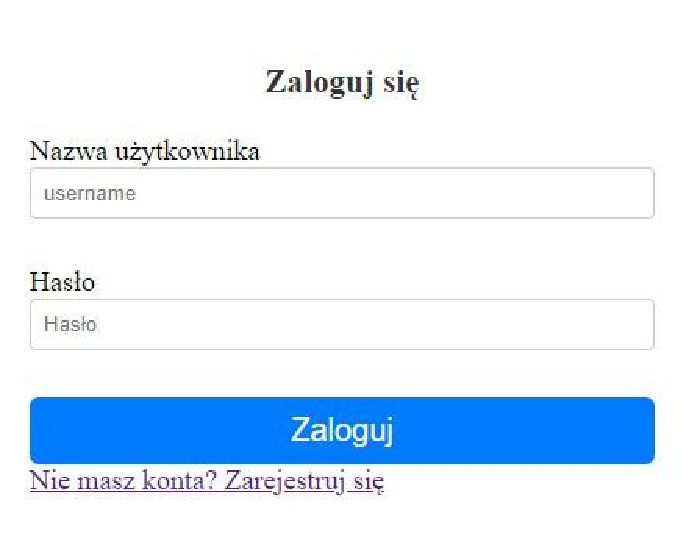
\includegraphics[width=0.35\textwidth]{rys05/view/login.pdf} & 
	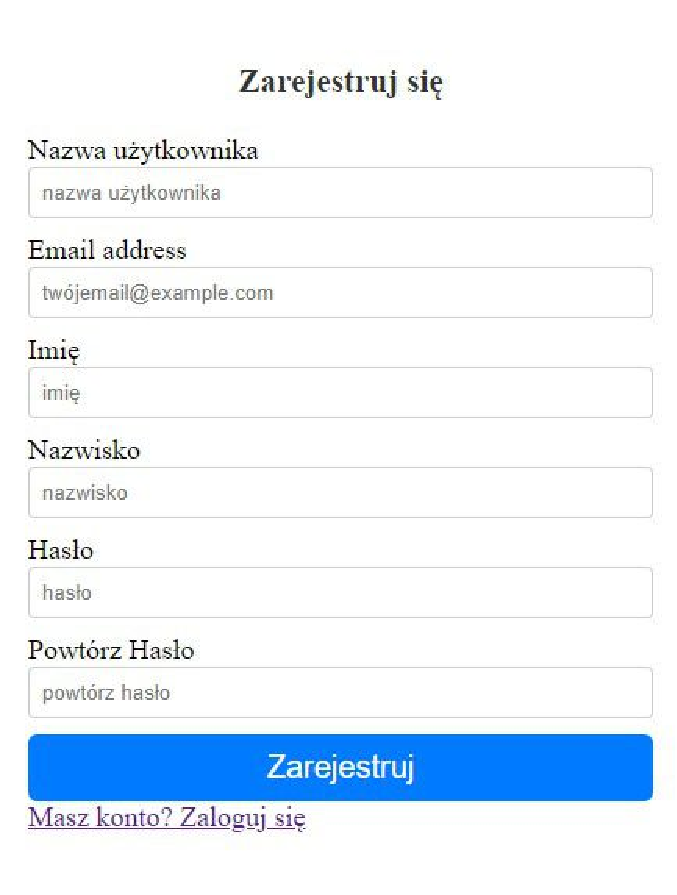
\includegraphics[width=0.35\textwidth]{rys05/view/register.pdf}
	\end{tabular}
  \caption{Widok W-1, Logowanie i Rejestracja a) logowanie, b) rejestracja}
  \label{authview:label}
\end{figure}


Widok W-1 formularzy logowania i rejestracji pokazany na rysunku \ref{authview:label} jest początkowym widokiem aplikacji. Każdy użytkownik musi się zalogować podając poprawne dane logowania na W-1a. W przypadku braku konta możliwa jest rejestracja klikając na odnośnik "`Nie masz konta? Zarejestruj się"' Po kliknięciu odnośnika następuje przekierowanie na W-1b. Po pomyślnym zarejestrowaniu następuje przekierowanie do W-1a. Możliwe jest tez kliknięcie odnośnika "`Masz już konto? Zaloguj się"' aby przejśc do formularza logowania W-1a.



\begin{figure}[htb]
  \centering
	\begin{tabular}{@{}lll@{}}
	a)\\
  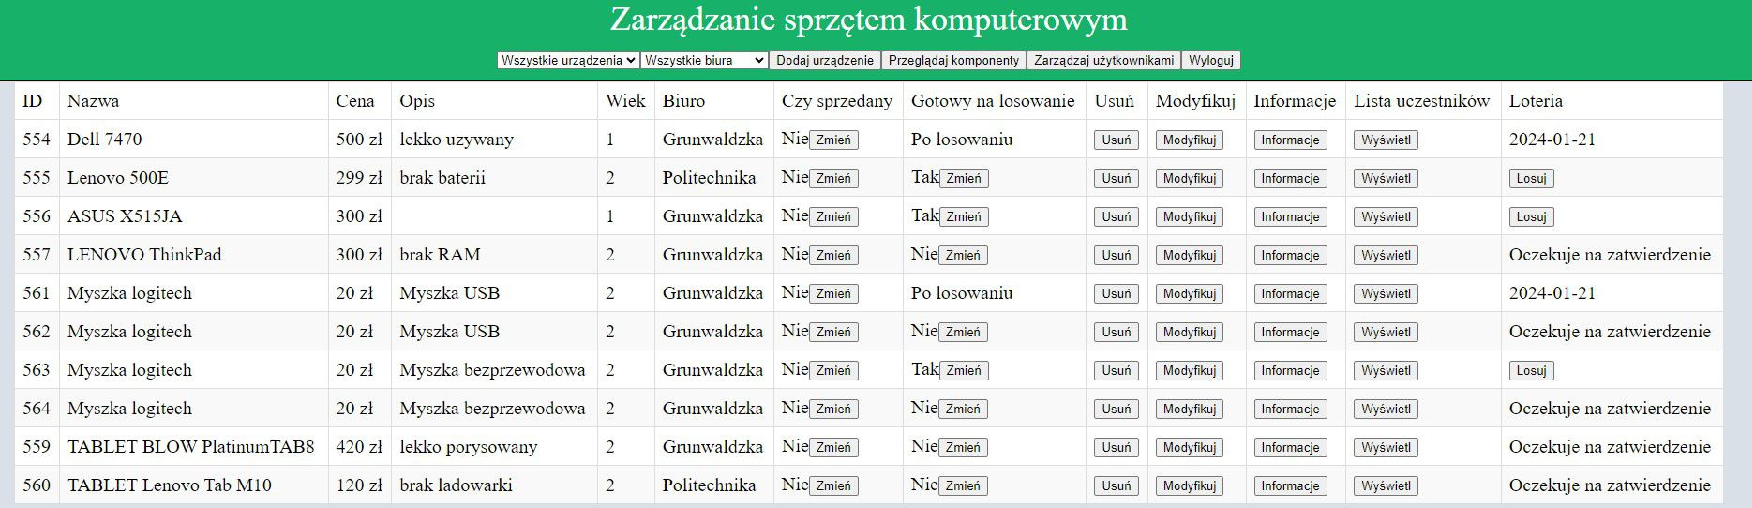
\includegraphics[width=\textwidth]{rys05/view/alldevices.pdf} \\
	
	b)\\
	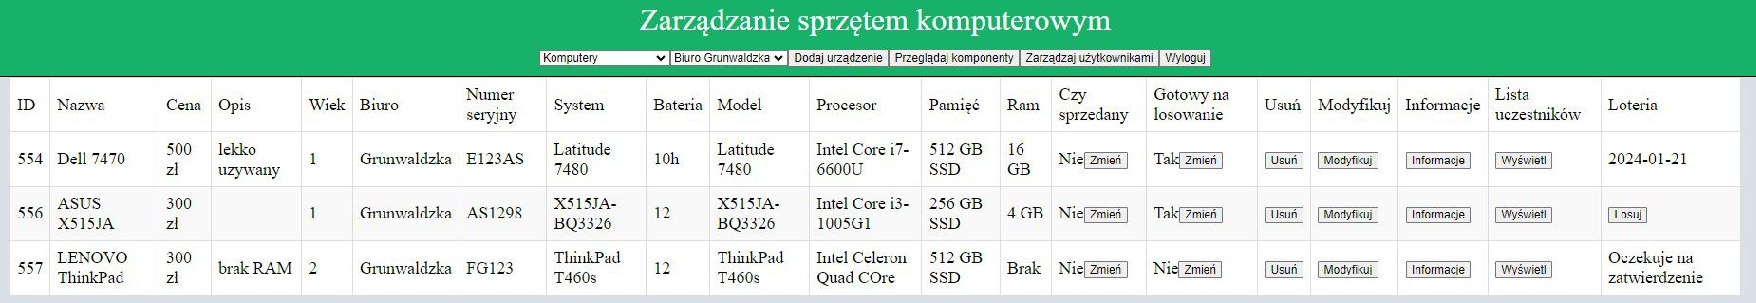
\includegraphics[width=\textwidth]{rys05/view/compGrun.pdf} \\
	c) \\
	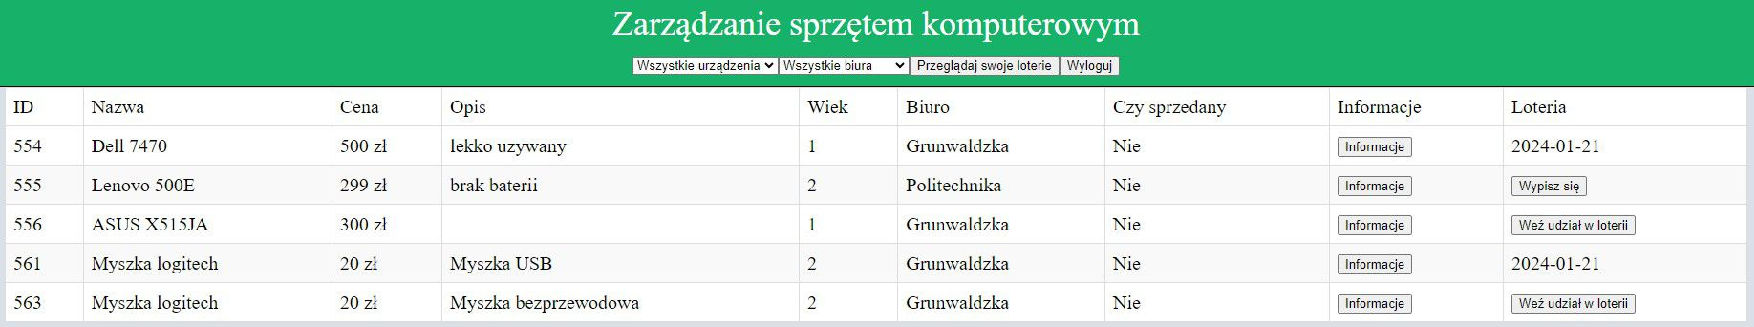
\includegraphics[width=\textwidth]{rys05/view/pracownikHome.pdf}
	\end{tabular}
  \caption{Widok W-2, Strona domowa a)Administrator bez filtrowania, b)Administrator z filtrowaniem c) Pracownik bez filtrowania}
  \label{home:label}
\end{figure}


Na rysunkach \ref{home:label} pokazany jest widok W-2 który posiada tabelę urządzeń z loteriami. Na każdym widoku istnieje przycisk wyloguj odpowiedzialny za wylogowywanie i przekierowanie do widoku W-1a \ref{authview:label}.Na widokach stron domowych W-2 możliwe jest filtrowanie urządzeń po typie urządzenia oraz po biurze w którym się znajdują oraz wyświetlanie szczegółowych informacji o urządzeniu. W widoku W-2b pokazane zostały tylko komputery które znajdują się w biurze Grunwaldzka. Wyśiwetlanie informacji o urządzeniu pokazuje na widoku wariant formularza W-3e dla odpowiadającego typu urządzenia: W-3a, W-3b, W-3c, rysunek \ref{forms:label}. Widok W-1a jest widokiem administratora który posiada wiele funkcjonalności:
\begin{itemize}
	\item Kliknięcie przycisku "`Dodaj urządzenie"' sprawia, że na ekranie wyświetlany jest formularz W-3a. Możliwa jest zmiana typu formularza na W-3b lub W-3c, która się odbywa poprzez wybór typu urządzenia z listy rozwijanej.
	\item Kliknięcie przycisku "`Przeglądaj komponenty"' sprawia, że następuje przekierowanie do widoku komponentów W-6.
	\item Kliknięcie przycisku "`Zarządzaj użytkownikami"' przekierowuje do widoku zarejestrowanych pracowników W-4a, rysunek \ref{manageUsers:label}
	\item Kliknięcie przycisku "`Zmień"' w kolumnie czy sprzedany ustawia status sprzętu na sprzedany lub nie. Jest to informacja czy sprzęt został dostarczony do pracownika.
	\item Kliknięcie przycisku w kolumnie "`Gotowy na losowanie"' możliwe jest tylko wtedy gdy losowanie się nie odbyło. Sprawia ono, że operacja "`Losuj"' w kolumnie loteria jest możliwa. Sprzęty które mają status gotowe do losowania są wyświetlane na widoku pracownika W-2c.
	\item Kliknięcie przycisku "`Usuń"' usuwa z systemu odpowiedni sprzęt.
	\item Kliknięcie przycisku "`Modyfikuj"' wyświetla na widoku wariant formularza W-3d, rysunek \ref{forms:label}. Wariant ten jest dostosowywany na podstawie odpowiadającemu mu rodzajowi sprzętu: W-3a, W-3b, W3-c.
	\item Kliknięcie przycisku "`Wyświetl"' w kolumnie "`Lista uczestników"' przekierowuje do widoku pracowników biorących udział w loterii wybranego sprzętu W-4b \ref{manageUsers:label}
	\item Kliknięcie przycisku "`Losuj"' w kolumnie loteria możliwe jest w przypadku gdy urządzenie jest gotowe do losowania oraz loteria się jeszcze nie odbyła. Następnie po kliknięciu przycisku ustawiana data losowania jest na dzisiejszą oraz losowany jest zwycięzca losowania. W przypadku braku uczestników losowanie nie odbędzie się.
\end{itemize}
Widok W-2c \ref{home:label} jest widokiem pracownika. Nie posiada on tak zaawansowanych funkcjonalności jak administrator. 
\begin{itemize}
	\item Kliknięcie przycisku w kolumnie loteria umożliwia zapisywanie lub wypisywanie z uczestnictwa w losowaniu. Zapis na loterie możliwy jest wtedy kiedy losowanie się jeszcze nie odbyło.
	\item Kliknięcie przycisku "`Przeglądaj swoje loterie"' przekierowuje do widoku W-5, rysunek \ref{lotteryHistory:label}. Widok ten posiada historię loterii dla aktualnie zalogowanego użytkownika.
\end{itemize}



\begin{figure}[htb]
  \centering
	\begin{tabular}{@{}lll@{}}
	a) & b) & c) \\
	\vtop{\vskip-2ex\hbox{\fbox{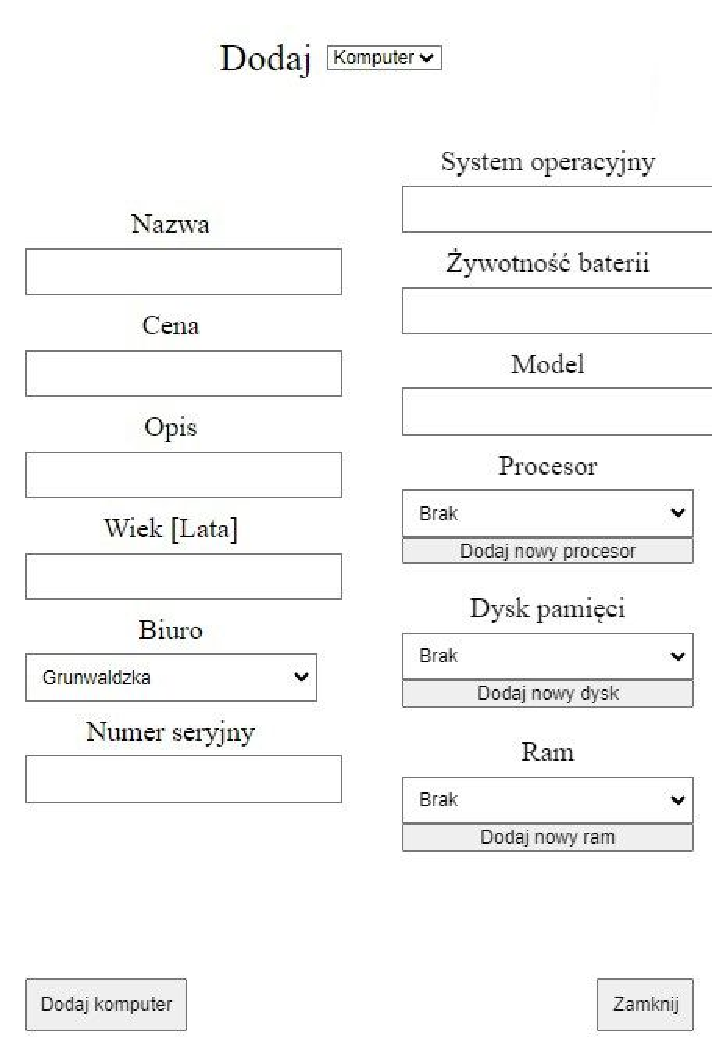
\includegraphics[width=0.3\linewidth]{rys05/view/addComputer.pdf}}}} & 
	\vtop{\vskip-2ex\hbox{\fbox{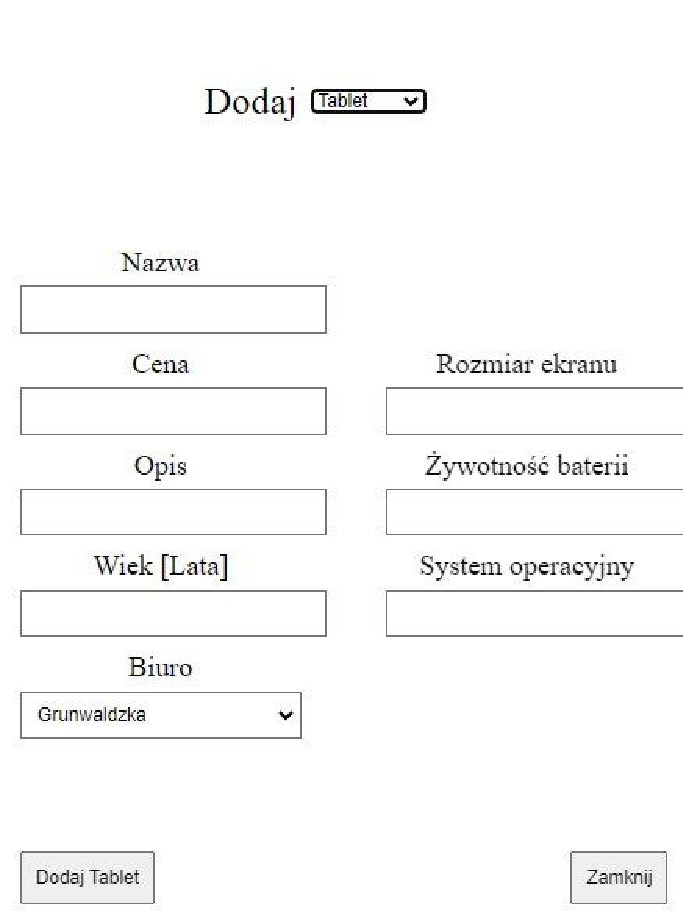
\includegraphics[width=0.3\linewidth]{rys05/view/addTablet.pdf}}}} & 
	\vtop{\vskip-2ex\hbox{\fbox{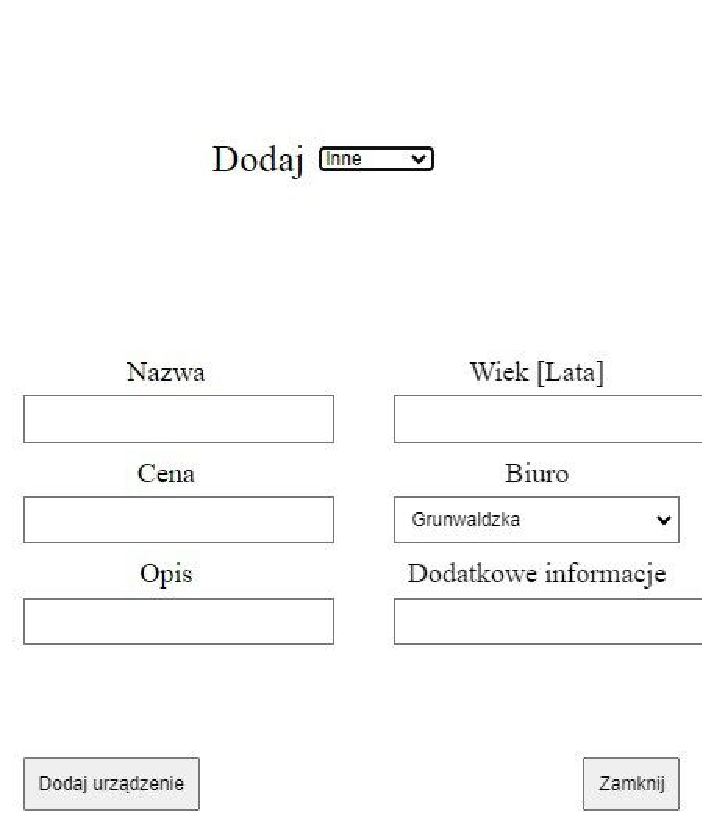
\includegraphics[width=0.3\linewidth]{rys05/view/addInne.pdf}}}} \\
 
	d) & e) \\
	
	\vtop{\vskip-2ex\hbox{\fbox{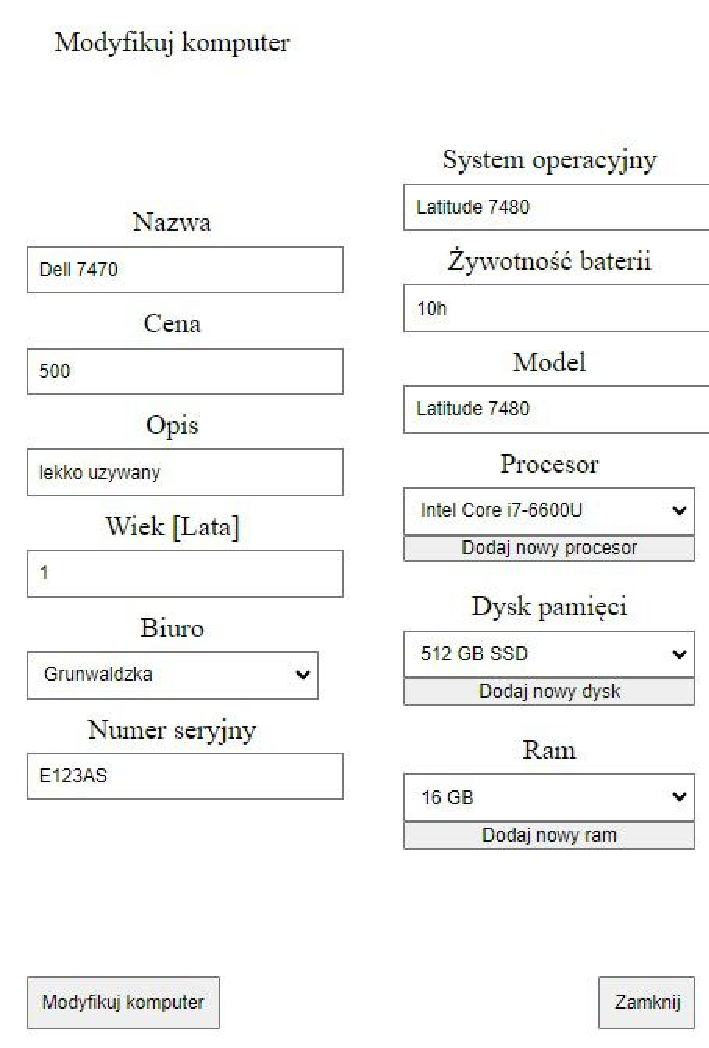
\includegraphics[width=0.3\linewidth]{rys05/view/modifyComp.pdf}}}} & 
	\vtop{\vskip-2ex\hbox{\fbox{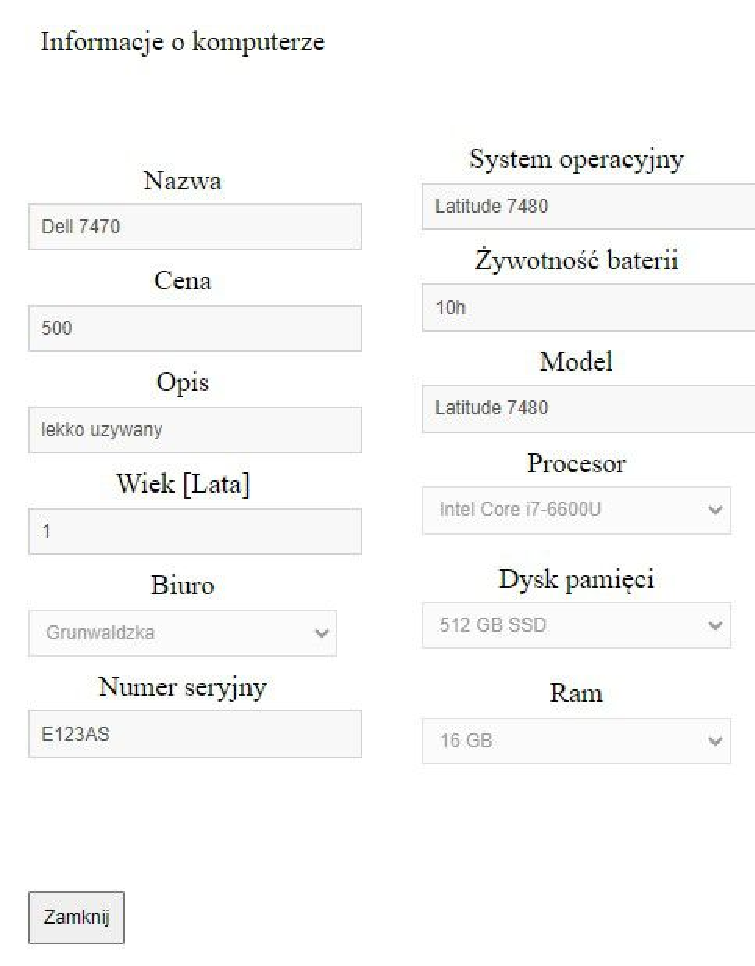
\includegraphics[width=0.3\linewidth]{rys05/view/infoComp.pdf}}}} & 
 
	\end{tabular}
  \caption{Widok W-3, Formularze a) dodawania komputera, b) dodawania tabletu, c) dodawania innego sprzętu, d) wariant modyfikacji, e) wariant informacji}
  \label{forms:label}
\end{figure}


Formularze W-3 ukazane na rysunku \ref{forms:label} wyświetlane są jako wyskakujące okno. Każdy z trzech formularzy W-3a, W-3b, W-3c oprócz wersji podstawowej odpowiadający mu wariant W-3d i W3e. Wariant podstawowy W-3a, W-3b, W-3c odpowiada za dodawanie nowego sprzętu. Możliwa jest zmiana typu sprzętu wybierając opcje z listy rozwijanej. Wariant W-3d służy to modyfikacji urządzenia i po jego pojawieniu się posiada aktualne dane urządzenia. Wariant W-3e odpowiada za wyświetlanie informacji o urządzeniu. Możliwość zmieniania danych na tym formularzu jest zablokowana. Formularz W-3a oraz odpowiadający mu W-3d posiada przyciski "`Dodaj nowy procesor"', "`Dodaj nowy dysk"', "`Dodaj nowy ram"'. W przypadku gdy administrator nie znajdzie z list rozwijanych interesującego go komponentu może kliknąć odpowiedni przycisk. Kliknięcie to powoduje pojawienie się formularza dla odpowiadającego go przycisku W-7a, W-7b, W-7c, rysunek \ref{compforms:label} Po dodaniu komponentu z widoku W-7 możliwe jest teraz z listy rozwijanej wybranie dodanego komponentu. \newline



\begin{figure}[htb]
  \centering
	\begin{tabular}{@{}lll@{}}
	a)\\
  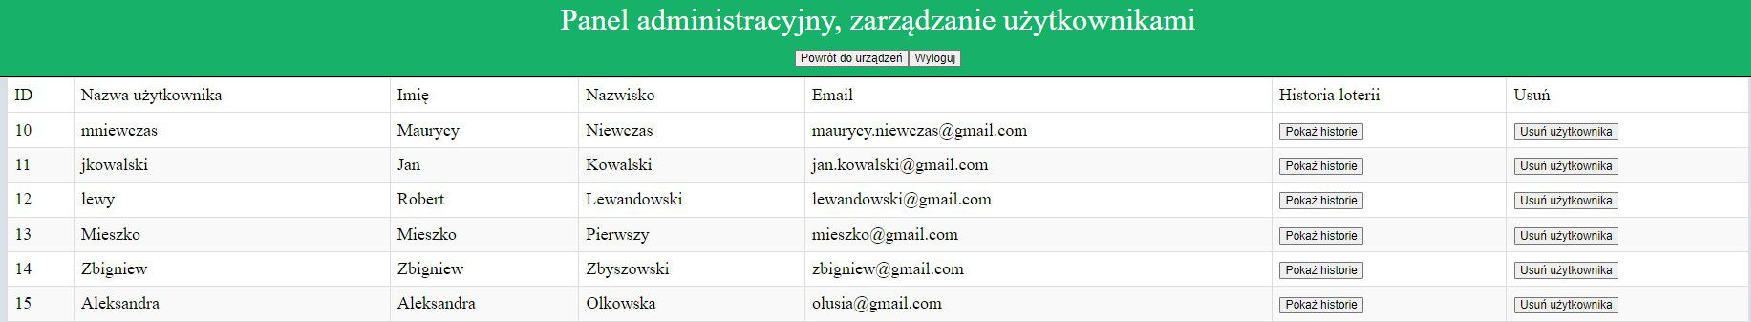
\includegraphics[width=\textwidth]{rys05/view/manageUsers.pdf} \\
	
	b)\\
	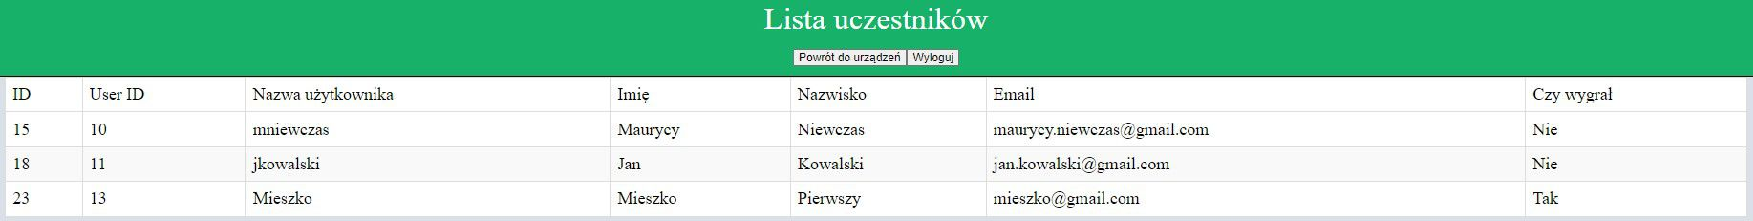
\includegraphics[width=\textwidth]{rys05/view/participation.pdf} \\
	
	\end{tabular}
  \caption{Widok W-4, Informacje o uzytkownikach a)Zarządzanie użytkownikami przez administratora, b)Przeglądanie uczestników losowania}
  \label{manageUsers:label}
\end{figure}


Widok W-4 \ref{manageUsers:label} posiada informacje o użytkownikach. W-4a jest widokiem dostępnym tylko dla administratora
\begin{itemize}
	\item kliknięcie przycisku powrót do urządzeń przekierowuje do strony domowej W-2 \ref{home:label}
	\item kliknięcie przycisku "`Pokaż historię"' w kolumnie Historia loterii przekierowuje do widoku historii loterii  W-5 \ref{lotteryHistory:label} dla odpowiadającego pracownika
	\item kliknicie przycisku "`Usuń użytkownika"' usuwa z systemu użytkownika
\end{itemize}
Widok W-4b też jest widokiem tylko dostępnym dla administratora. Posiada on listę uczestników oraz informacje o wygranej przegranej każdego poszczególnego uczestnika dla wybranej loterii.\newline


\begin{figure}[h]
		\centering
    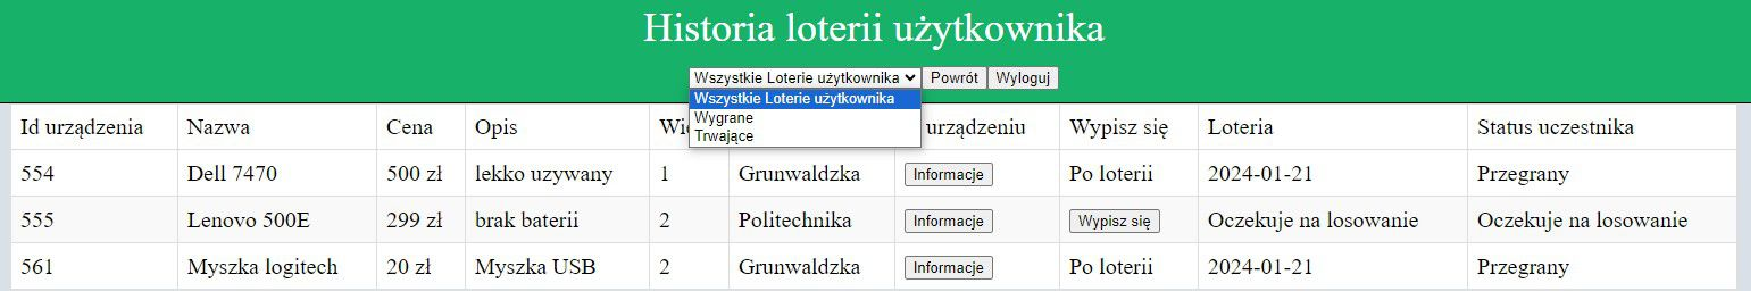
\includegraphics[width=\linewidth]{rys05/view/lotteryHistory.pdf}
    \caption{Widok W-5, Historia loteri pracownika}
    \label{lotteryHistory:label}
\end{figure}


Widok W-5 pozwala wyświetlić historię loterii użytkownika, rysunek \ref{lotteryHistory:label}. Pozwala on na pracownikowi przeglądanie własnej historii. Administrator może skorzystać z tego widoku aby sprawdzić historię loterii wybranego pracownika.
\begin {itemize}
	\item Możliwe jest tutaj filtrowanie loterii na podstawie statusu uczestnika. Są dostępne 3 opcje: "`Wszystkie loterie użytkownika"', "`Wygrana"' i "`Trwająca"'
	\item Kliknięcie przycisku "`Informacje"' wyświetla szczegółowe informacje o sprzęcie, wariant W-3e dla formularzy W-3a, W-3b, W-3c, rysunek \ref{forms:label} 
	\item Kliknięcie przycisku "`Wypisz się"' możliwe jest wtedy kiedy loteria się jeszcze nie odbyła. Po kliknięciu tego przycisku pracownik rezygnuje z uczestnictwa w losowaniu wybranego sprzętu.
\end{itemize} 




\begin{figure}[h]
		\centering
    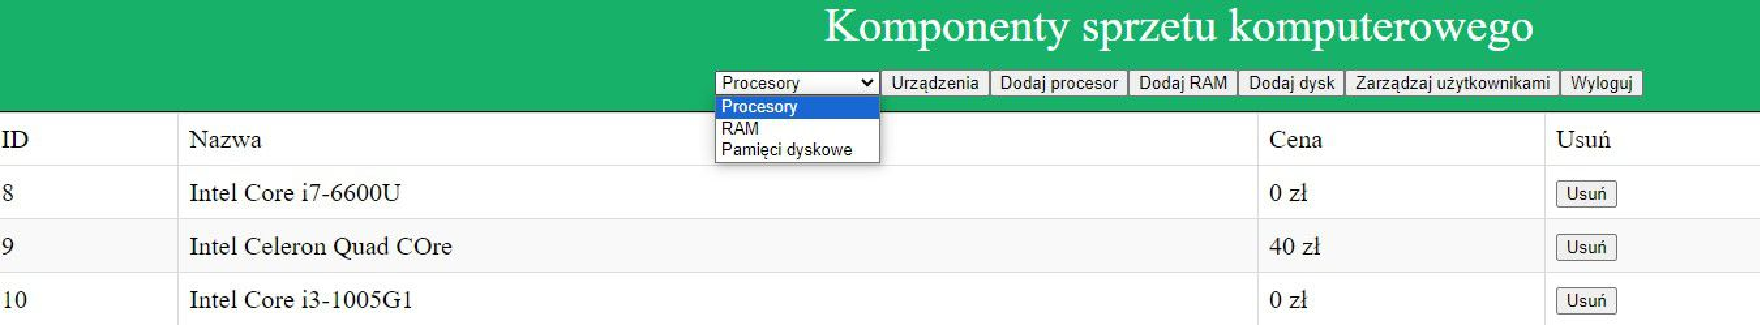
\includegraphics[width=\linewidth]{rys05/view/components.pdf}
    \caption{Widok W-6, Widok komponentów komputera}
    \label{components:label}
\end{figure}

Widok W-6 jest dostępny dla administratora. Pozwala mu na oszacowanie ceny sprzętu patrząc jakie komponenty mają cenę. Możliwe jest wybranie z listy rozwijanej jakiego rodzaju komponenty mają być wyświetlane. Do wyboru są: procesory, pamięci RAM oraz pamięci dyskowe.
\begin{itemize}
	\item Kliknięcie przycisku "`Dodaj procesor"' wyświetli formularz W-7a \ref{compforms:label} odpowiedzialny za dodanie procesora.
	\item Kliknięcie przycisku "`Dodaj RAM"' Wyświetli formularz W-7b \ref{compforms:label} odpowiedzialny za dodanie pamięci RAM.
	\item Kliknięcie przycisku "`Dodaj dysk"' Wyświetli formularz W-7c \ref{compforms:label} odpowiedzialny za dodawanie dysku pamięci.
	\item Kliknięcie przycisku "`Zarządzaj użytkownikami"' przekieruje do widoku W-4a \ref{manageUsers:label}
	\item Klikniecie przycisku usuń spowoduje usunięcie komponentu. Komputer posiadający usuwany komponent ustawia identyfikator odpowiedniego komponentu na wartość "`null"'
\end{itemize} 

W przypadku dodaniu komponentu, którego nazwa już istnieje następuje modyfikacja ceny.


\begin{figure}[htb]
  \centering
	\begin{tabular}{@{}lll@{}}
	a) & b) & c) \\
  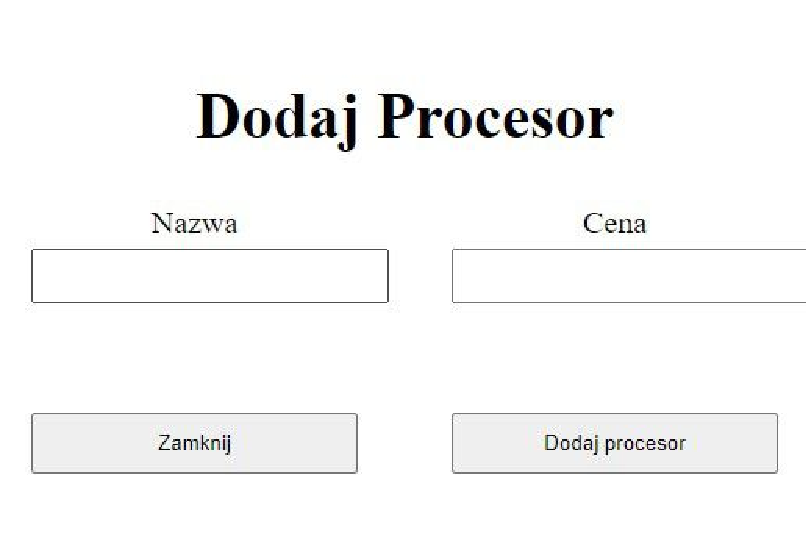
\includegraphics[width=0.35\textwidth]{rys05/view/addProc.pdf} & 
	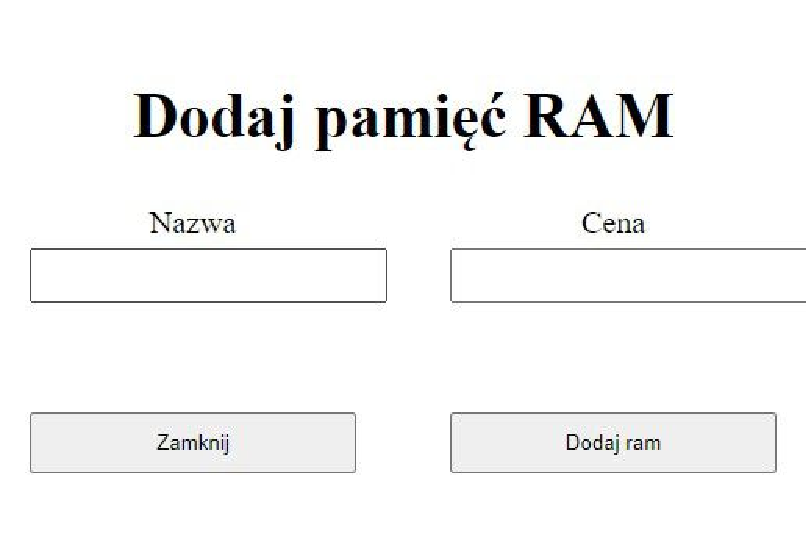
\includegraphics[width=0.35\textwidth]{rys05/view/addRam.pdf} &
	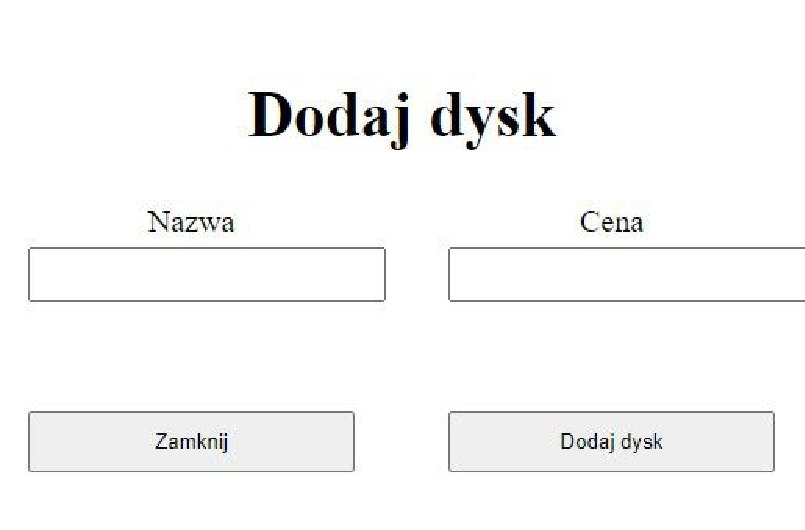
\includegraphics[width=0.35\textwidth]{rys05/view/addStorage.pdf}
	\end{tabular}
  \caption{Widok formularzy komponentów W-7, a) procesor, b) ram, c) dysk pamięci}
  \label{compforms:label}
\end{figure}

Widok W-7 \ref{compform:label} odpowiedzialny jest za widoki formularzy komponentów. Formularze te mogą zostać wyświetlone po kliknięciu odpowiedniego przycisku na widoku W-6 \ref{components:label} lub z przycisku dostępnego na formularzu komputera(widok W-5a, W-5e, \ref{forms:label}.




\chapter{Testy aplikacji}

\section{Wykorzystane technologie}

Do przetestowania aplikacji wykorzystano \textbf{Postmana} i \textbf{Lighthouse} \ref{tab:zestawienie_narzędzi}. Postman pozwoli sprawdzić czy zapytania oraz logika działają prawidłowo. Lighthouse pozwoli przeanalizować jakość strony internetowej


\section{Testowanie Restowych zapytań przy pomocy Postmana}

Wykorzystując Postmana można na bieżąco monitorować stan aplikacji. Wykonując odpowiednie zapytania można sprawdzić w jaki sposób odpowiada aplikacja serwerowa na dane zapytanie. Ułatwia to pracę i wysyłanie zapytań z aplikacji klienckiej. Przetestowano każde z dostępnych zapytań zdefiniowane w tabeli \ref{tab:rest1} i \ref{tab:rest2}. Testowanie odbywało się na bieżąco z rozwojem systemu. Umożliwiło to szybką identyfikacje problemów.

\begin{figure}[htb]
  \centering
	\begin{tabular}{@{}llll@{}}
	a) & b) & c) & d) \\
	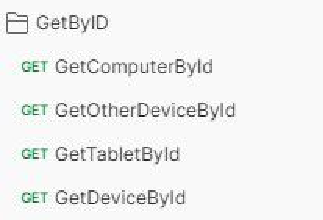
\includegraphics[width=0.17\linewidth]{rys06/struct/byid.pdf} & 
	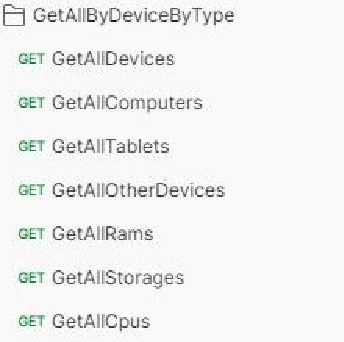
\includegraphics[width=0.17\linewidth]{rys06/struct/alldevices.pdf} & 
	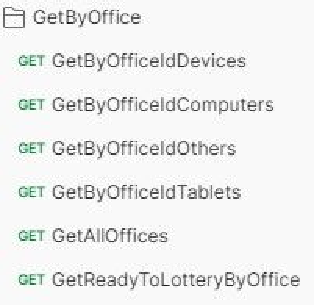
\includegraphics[width=0.17\linewidth]{rys06/struct/byOffice.pdf} & 
	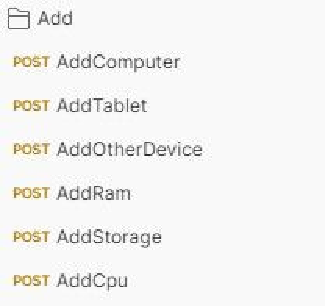
\includegraphics[width=0.17\linewidth]{rys06/struct/add.pdf} \\
 
	e) & f) & g) & h)\\
	
	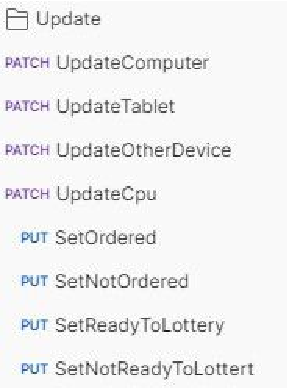
\includegraphics[width=0.17\linewidth]{rys06/struct/update.pdf} & 
	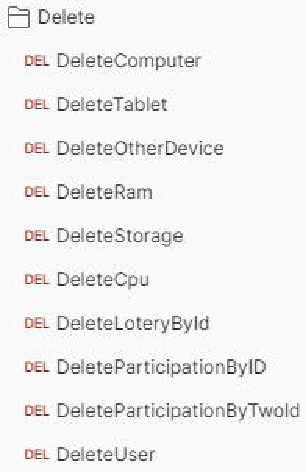
\includegraphics[width=0.17\linewidth]{rys06/struct/del.pdf} & 
	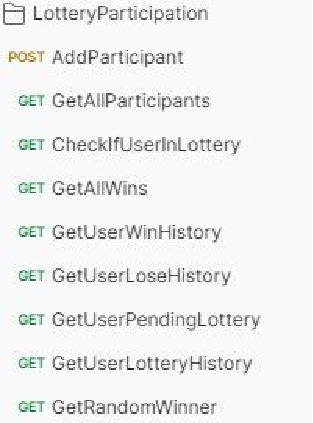
\includegraphics[width=0.17\linewidth]{rys06/struct/lottery.pdf} & 
	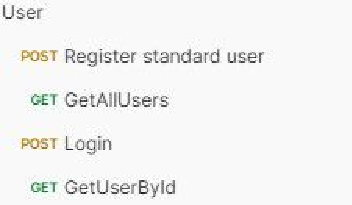
\includegraphics[width=0.17\linewidth]{rys06/struct/user.pdf} \\
 
 
	\end{tabular}
  \caption{Struktura testów a) po id, b) wszystkie urządzenia, c) sortowanie po biurze, d) dodawanie, e) aktualizacja, f) usuwanie, g) związane z loterią, h) związane z uzytkownikiem}
  \label{postmanStruct:label}
\end{figure}
\newpage

\subsection {Wybrane scenariusze testowe}


\subsubsection{Pobieranie informacji o sprzęcie}
Na scenariuszu testowym 1 \ref{getByIdTest:label} przetestowano pobieranie informacji o urządzeniu. Wykorzystując zapytanie \texttt{localhost:8080/devices/{id}} metodą GET uzyskano na scenariuszu testowym 1a i 1b status 200 OK. Wyświetlane informacje świadczą o poprawności działania funkcjonalności pobierania informacji o sprzęcie. W scenariuszu 1a zostały wyświetlone informacje o komputerze a w 1b o innym urządzeniu. Odpowiedź zapytania jest zależna od tego jakie urządzenie o zadanym ID ma typ. Możliwe jest coś takiego po wykorzystaniu schematu dziedziczenia które dostarcza unikalnych kluczy dal poszczególnych typów sprzętów. Więcej na ten temat napisano w rozdziale \ref{dzedziczenie_hibernate:label}.


\begin{figure}[htb]
  \centering
	\begin{tabular}{@{}ll@{}}
	a) & b) \\
  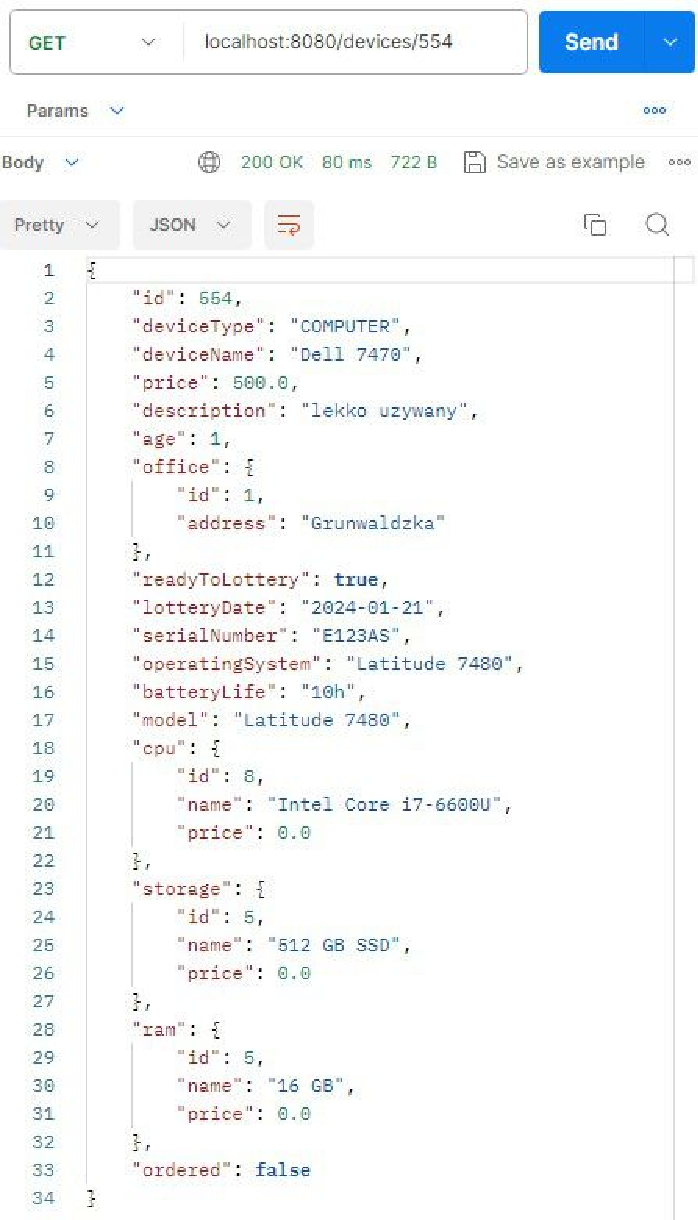
\includegraphics[width=0.5\textwidth]{rys06/postmanTest/compById.pdf} & 
	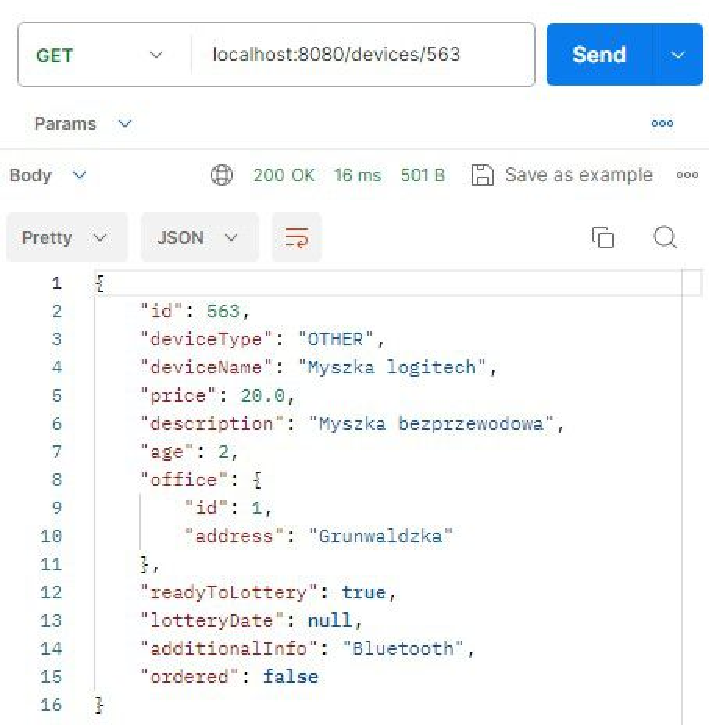
\includegraphics[width=0.5\textwidth]{rys06/postmanTest/otherById.pdf}
	\end{tabular}
  \caption{Scenariusz testowy 1,pobieranie informacji o urządzeniu, a) komputer, b) inne urządzenie}
  \label{getByIdTest:label}
\end{figure}



\subsubsection{Dodawanie i modyfikowanie urządzenia}
Na scenariuszu testowym 2 \ref{addModTest:label} najpierw dodano a potem zmodyfikowano dodane urządzenie. W obu przypadkach dane zostały wysłane jako JSON. W 2a po wysłaniu żądania metodą POST uzyskano status HTTP 201 Created. Oznacza to że urządzenie zostało poprawnie dodane do systemu. W dolnej części 2a widać jakie urządzenie zostało stworzone i jakie ma parametry. Scenariusz 2b modyfikuje utworzone w 2a urządzenie.Potrzebuje do tego oprócz danych zmieniających sprzęt ID urządzenia. ID jest przekazywane przez ścieżkę url. Możliwa jest modyfikacja pól w ten sposób by były miały wartość null. Skorzystano tutaj z metody PATCH która modyfikuje istniejący element.

\begin{figure}[htb]
  \centering
	\begin{tabular}{@{}ll@{}}
	a) & b) \\
  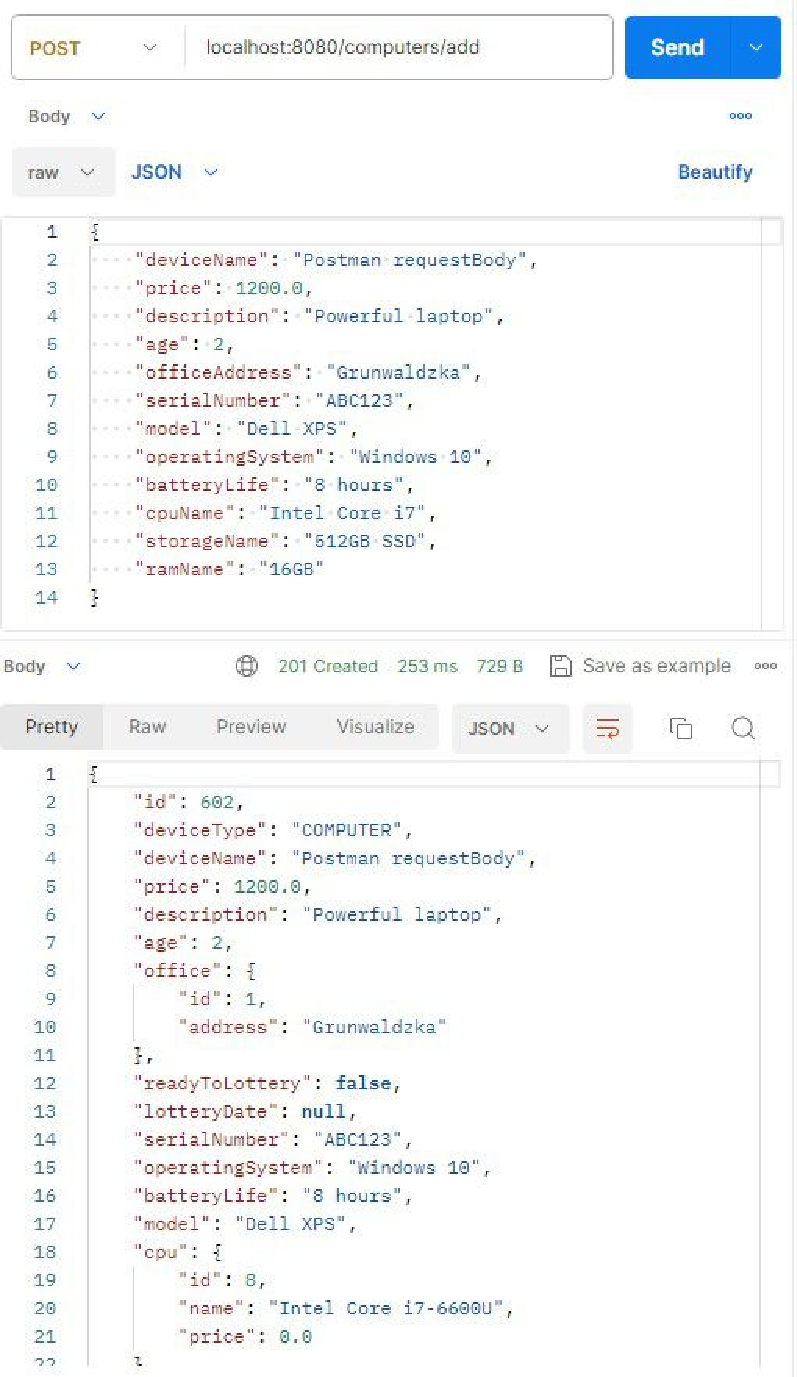
\includegraphics[width=0.45\textwidth]{rys06/postmanTest/addComp.pdf} & 
	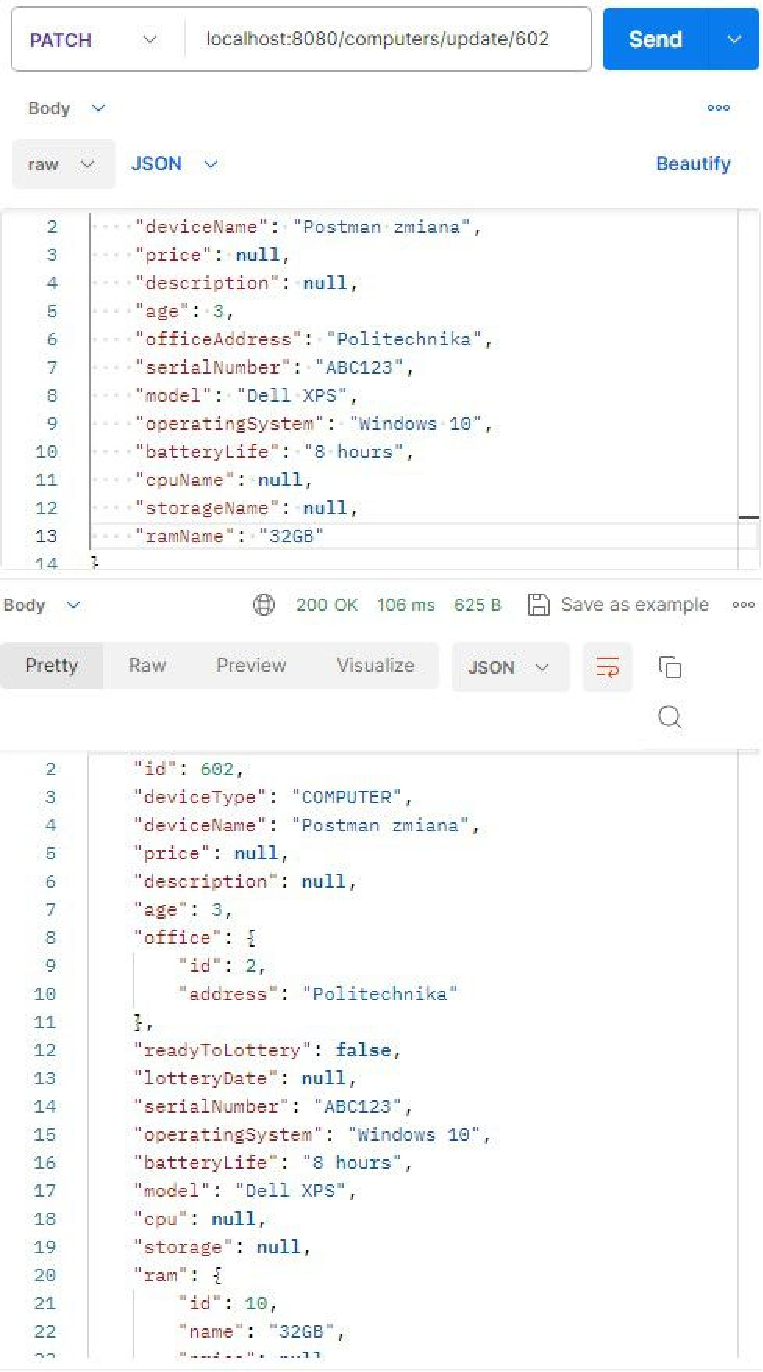
\includegraphics[width=0.45\textwidth]{rys06/postmanTest/patch.pdf}
	\end{tabular}
  \caption{Scenariusz testowy 2,Dodawanie i modyfikowanie komputera, a) dodawanie, b) modyfikacja}
  \label{addModTest:label}
\end{figure}



\subsubsection{Usuwanie urządzenia}
W scenariuszu testowym 3 \ref{deleteTest:label} pokazano w jaki sposób jest usuwane urządzenie. Do usunięcia urządzenia potrzebne jest ID, które przekazywane jest przez ścieżkę url. Po skorzystaniu z metody DELETE uzyskiwany jest status http 200 OK, który oznacza, że urządzenie zostało pomyślnie usunięte.


\begin{figure}[h]
		\centering
    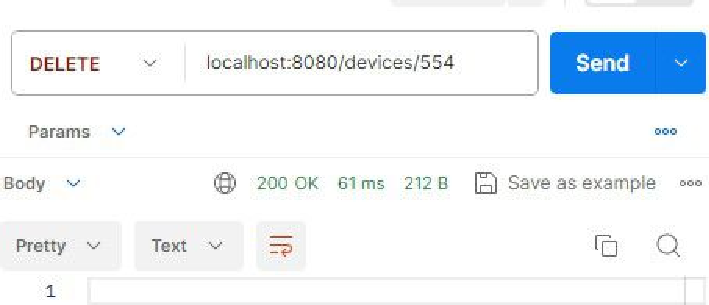
\includegraphics[width=0.45\linewidth]{rys06/postmanTest/delete.pdf}
    \caption{Scenariusz testowy 3, Usuwanie urządzenia po ID}
    \label{deleteTest:label}
\end{figure}


\subsubsection{Losowanie zwycięzcy}

Jedną z głównych funkcjonalności aplikacji jest przeprowadzenie losowania. Scenariusz testowy 3 \ref{winnerTest:label} pokazuje w jaki sposób jest przeprowadzane losowanie. W przypadku kiedy loteria posiada zapisanych użytkowników, losowany jest zwycięzca, jako status HTTP uzyskiwany jest 200 OK. W scenariuszu 3b pokazano przypadek kiedy na loterię nie został zapisany żaden pracownik lub loteria nie została otworzona. Wtedy status HTTP jest 204 No Content. 


\begin{figure}[htb]
  \centering
	\begin{tabular}{@{}ll@{}}
	a) & b) \\
  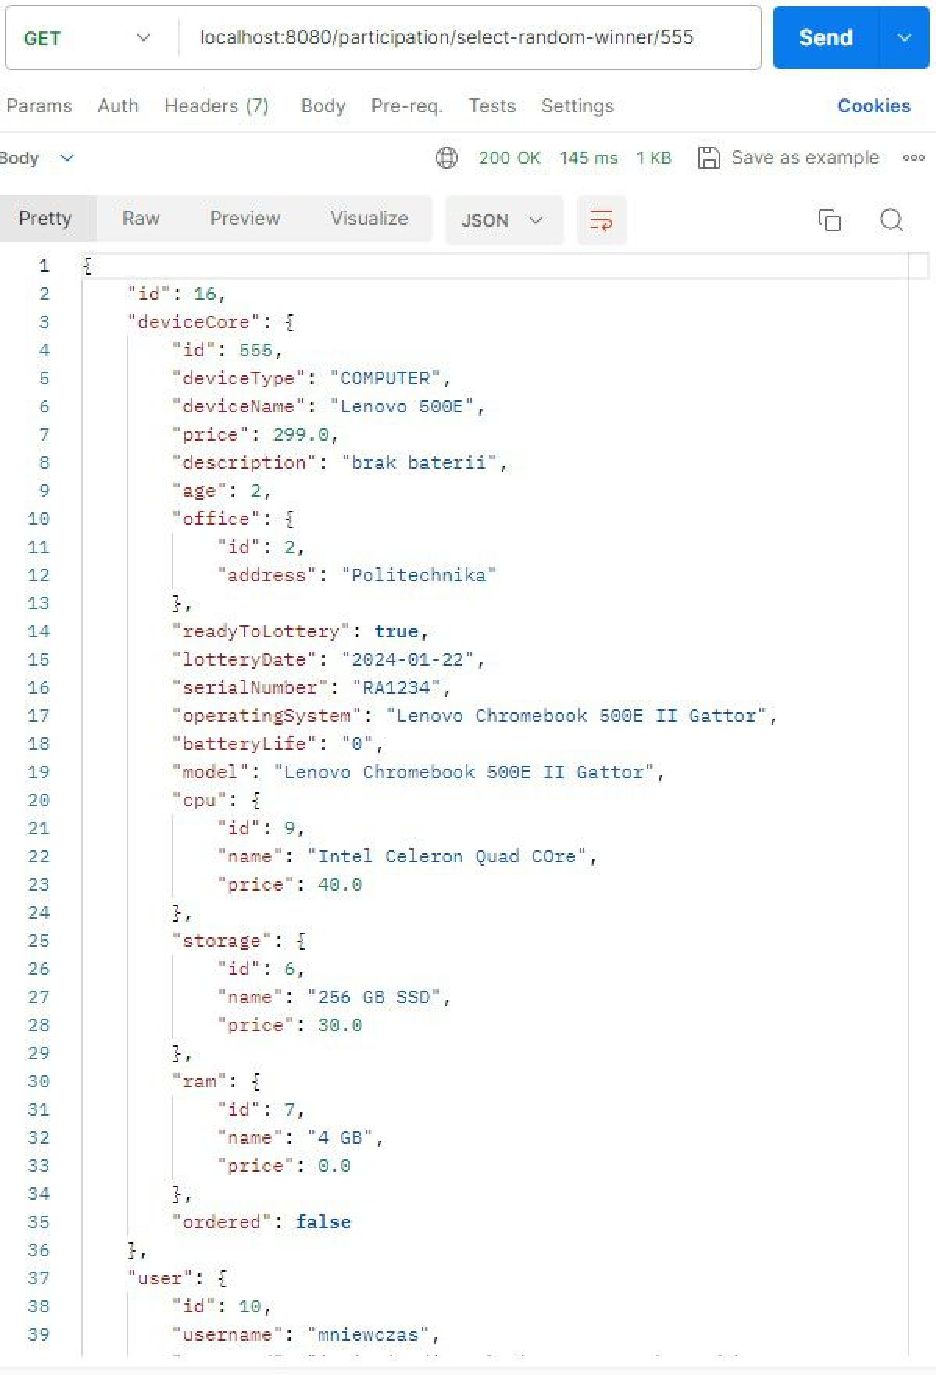
\includegraphics[width=0.5\textwidth]{rys06/postmanTest/winner.pdf} & 
	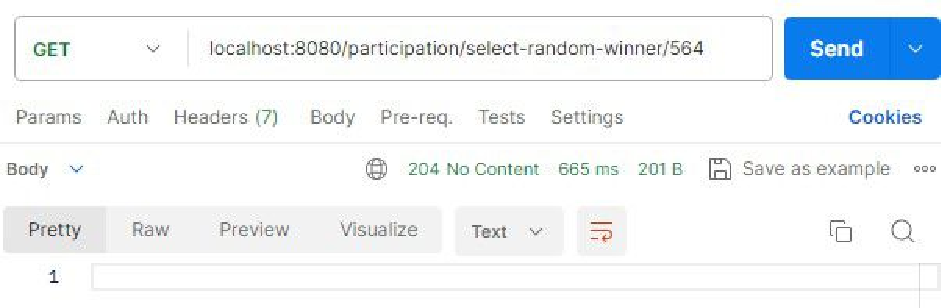
\includegraphics[width=0.5\textwidth]{rys06/postmanTest/badWinner.pdf}
	\end{tabular}
  \caption{Scenariusz testowy 3,Losowanie zwycięzcy, a) powodzenie, b) niepowodzenie}
  \label{winnerTest:label}
\end{figure}

\newpage
\subsubsection{Rejestracja użytkownika}
Scenariusz testowy 4 \ref{registerTest:label} pokazuje jak działa rejestracja użytkownika. Po utworzeniu takiego użytkownika zwracany jest status HTTP 201 Created. Użytkownik taki zapisywane hasło ma w postaci zaszyfrowanej.

\begin{figure}[h]
		\centering
    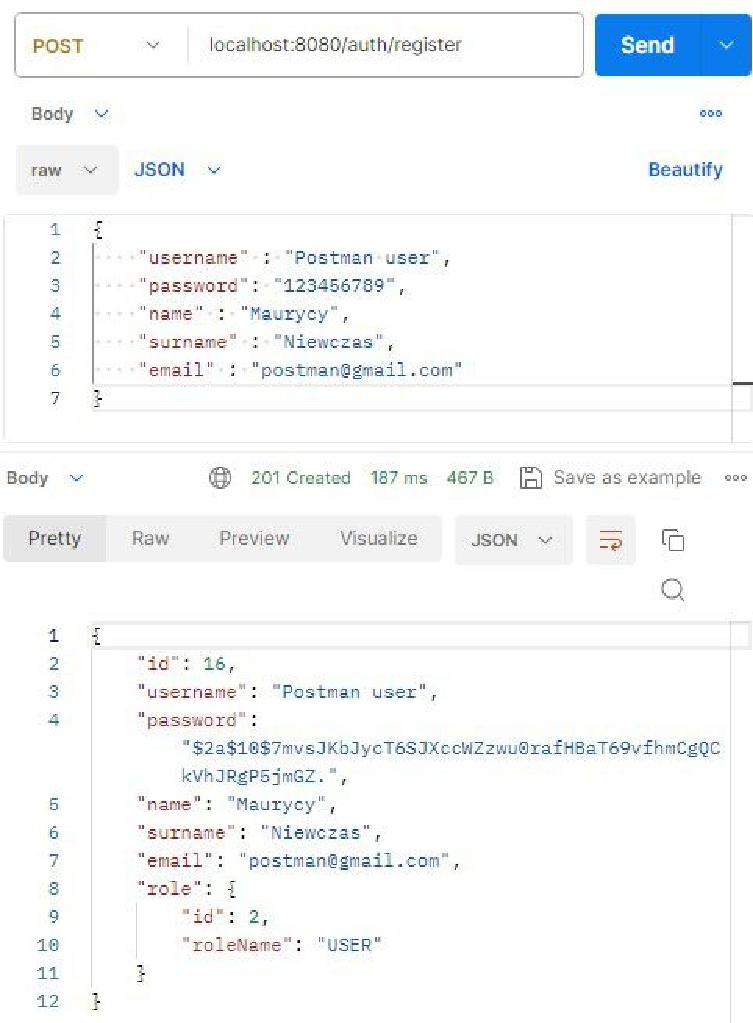
\includegraphics[width=0.7\linewidth]{rys06/postmanTest/register.pdf}
    \caption{Scenariusz testowy 4, Rejestracja użytkownika}
    \label{registerTest:label}
\end{figure}

\newpage
\section{Testowanie jakości strony internetowej systemu przy użyciu Lighthouse}

Wykorzystanie Lighthouse \ref{tab:zestawienie_narzędzi} pozwala na zbadanie wydajności, dostępności i dobrych praktyk strony internetowej. Testowany widok był strony domowej, ponieważ na niej dzieje się większość logiki systemu. Testowanie odbyło się w dwóch wariantach: strony domowej administratora i strony domowej pracownika \ref{lh:label}

\begin{figure}[htb]
  \centering
	\begin{tabular}{@{}ll@{}}
	a) & b) \\
  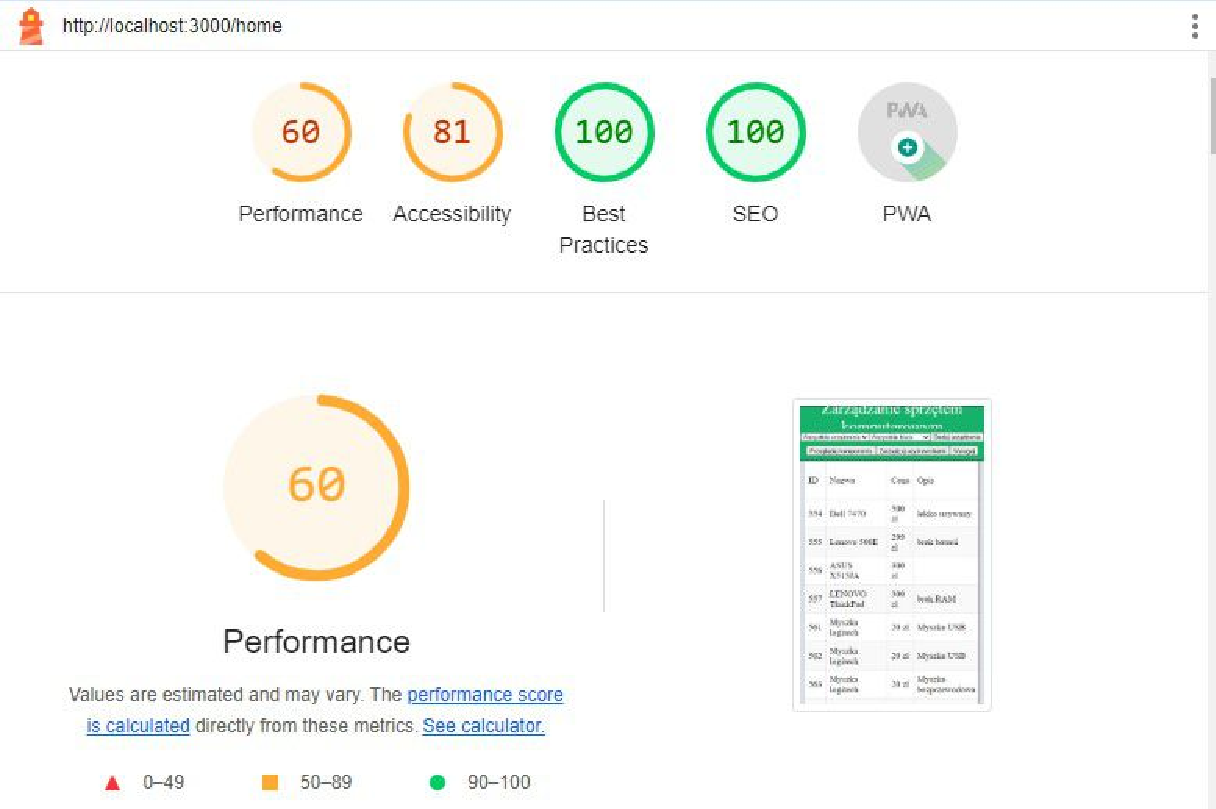
\includegraphics[width=0.5\textwidth]{rys06/lighthouse/adminLightHouse.pdf} & 
	\includegraphics[width=0.5\textwidth]{rys06/lighthouse/workerLightHouse.pdf}
	\end{tabular}
  \caption{Test Lighthouse strony domowej, a) administratora, b) pracownika}
  \label{lh:label}
\end{figure}

Wnioskując z testu widok aplikacji ma satysfakcjonujące parametry.
\begin{itemize}
\item \textbf{Wydajność (Performance)} jest na średnim poziomie. Pokazuje to że aplikacja mogła by być bardziej zoptymalizowana pod względem wydajności
\item \textbf{Dostępność (Accessibility} jest na wysokim poziomie. Oznacza to, że osoby z różnymi niepełnosprawnościami nie miałyby większego problemu z posługiwaniem się aplikacją. Jednak tutaj jest możliwość optymalizacji by osiągnąć większy stopień zadowolenia tych użytkowników.
\item \textbf{Dobre praktyki (Best Practices)} pokazuje, że test przeszedł test dobrych praktyk i storn a jest zgodna ze standardami.
\item \textbf{SEO} - Pokazuje, że strona jest zoptymalizowana pod kątem wyszukiwarek internetowych
\end{itemize}


%więcej rozdziałów

% LITERATURA (zostanie wygenerowana automatycznie)
%UWAGA: bibliotekę referencji należy przygotować samemu. Dobrym do tego narzędziem jest JabRef.
%       JabRef oferuje jednak większą liczbę typów rekordów niż obsługuje BibTeX.
%       Proszę nie deklarować rekordów o typach nieobsługiwanych przez BibTeX.
%       Formatowania wykazu literatury i cytowań odbywać się ma zgodnie z zadeklarowanym stylem.
%       Zalecane są style produkujące numeryczne cytowania (w postaci [1], [2,3]).
%       Takim stylem jest np. plabbrv
\bibliographystyle{plabbrv}
%       Aby zapanować nad odstępami w wykazie literatury można posłużyć się poniższą komendą
\setlength{\bibitemsep}{2pt} % - zacieśnia wykaz
%       Pozycja Literatura pojawia się w spisie treści nieco inaczej niż spisy rysunków, tabel itp.
%       Aby zachować właściwe odstępy należy użyć poniższej komendy
\addtocontents{toc}{\addvspace{2pt}} % ustawiamy odstęp w spisie treści przed pozycją Literatura 
%       Nazwę pliku przygotowanej biblioteki wpisuje się bez rozszerzenia .bib
%       (linia poniżej załaduje rekordy z pliku "dokumentacja.bib")
\bibliography{dokumentacja}
\appendix

% Jeśli w pracy pojawiać się ma indeks, należy odkomentować poniższe linie
%%\chapterstyle{noNumbered}
%%\phantomsection % sets an anchor
%%\addcontentsline{toc}{chapter}{Indeks rzeczowy}
%%\printindex

\end{document}
